%%%%%%%%%%%%%%%%%%%%%%%%%%%%%%%%%%%%%%%%%%%%%%%%%%%%%%%%%%%% 
% This is the official template for theses and seminar papers from the Chair for Information Systems for Sustainable Society (IS3) at the University of Cologne

%
%PREAMBLE
%%%%%%%%%%%%%%%%%%%%%%%%%%%%%%%%%%%%%%%%%%%%%%%%%%%%%%%%%%%%%

\documentclass[a4paper, oneside, 12pt, hidelinks]{article}
\usepackage[left=4cm, right=2.5cm, top=2.5cm, bottom=2.5cm]{geometry} 
% set line spacing
\usepackage{setspace}
\setstretch{1.5}
\usepackage[utf8]{inputenc}
\usepackage[T1]{fontenc}
\usepackage{graphicx}
\usepackage{longtable}
\usepackage{hyperref}
\usepackage{caption}
\usepackage{booktabs}
\usepackage{pifont}
\usepackage{placeins}
\usepackage{array}
\usepackage{tikz}
\usetikzlibrary{arrows.meta}

% pgfplots provides the \begin{axis} environment used in several figures
\usepackage{pgfplots}
\pgfplotsset{compat=1.18}

\usepackage{textgreek}
\newcommand{\cmark}{\ding{51}}
% Pakete laden
\usepackage{amssymb} % Für das Standard-Häkchen (\checkmark)
\usepackage{pifont}  % Für Sonderzeichen und Symbole

% Eigene Befehle definieren
\newcommand{\xmark}{\ding{55}} % Passendes Kreuzchen

% set indentation size
% check mark
% set indentation size
\usepackage{indentfirst}
\setlength{\parindent}{30pt}
% set font size to times
\usepackage{times}
% set title font sizes
\usepackage{titlesec}
% set \section font size to 14
\titleformat{\section}
    {\normalfont\bfseries\fontsize{14}{20}\selectfont}
    {\thesection}{1em}{}
% Customize \section spacing
\titlespacing*{\section}
    {0pt}   % Left indentation
    {10pt}  % Space before the title
    {0pt}   % Space after the title

% set \section font size to 13
\titleformat{\subsection}
    {\normalfont\bfseries\fontsize{13}{20}\selectfont}
    {\thesubsection}{1em}{}
% Customize \subsection spacing
\titlespacing*{\subsection}
    {0pt}   % Left indentation
    {10pt}  % Space before the title
    {0pt}   % Space after the title

% set \section font size to 13
\titleformat{\subsubsection}
    {\normalfont\bfseries\fontsize{12}{20}\selectfont}
    {\thesubsubsection}{1em}{}
% Customize \subsubsection spacing
\titlespacing*{\subsubsection}
    {0pt}   % Left indentation
    {10pt}  % Space before the title
    {0pt}   % Space after the title

% set headers
\usepackage{fancyhdr}
\pagestyle{fancy}
\fancyhead{}
\fancyfoot{}
\fancyhead[L]{\textsl{\leftmark}}
\fancyhead[R]{\thesisauthor}
\fancyfoot[C]{\thepage}
\renewcommand{\headrulewidth}{0.4pt}
\renewcommand{\footrulewidth}{0pt}

% set APA citation style
\usepackage[backend=biber,style=apa]{biblatex}
\addbibresource{references.bib} % Zotero export (Better BibTeX)
%\addbibresource{Bibliography.bib} % optional: keep if you also use this file
\pagenumbering{gobble}

%%%%%%%%%%%%%%%%%%%%%%%%%%%%%%%%%%%%%%%%%%%%%%%%%%%%%%%%%%%%%
%THESIS Parameters 
%%%%%%%%%%%%%%%%%%%%%%%%%%%%%%%%%%%%%%%%%%%%%%%%%%%%%%%%%%%%%

\title{LLM Workflow or Agent? A Task-Level Architecture Decision Framework for Agentic Workplace Automation}

\newcommand{\thesisdate}{\today} % TODO: durch das Abgabedatum ersetzen
\date{\thesisdate} % sorgt dafuer, dass \thesisdate auf der Titelseite landet
\newcommand{\thesisauthor}{Steffen Niesmann} %input name
\newcommand{\studentID}{7431253} %input student ID
\newcommand{\thesistype}{Master Thesis} % Set either to Bachelor or Master
\newcommand{\supervisor}{Univ.-Prof. Dr. Detlef Schoder}
\newcommand{\cosupervisor}{Tom Celig}

% Signature line
\newcommand{\signature}{%
    \vspace{2cm}%
    \noindent\rule{0.5\textwidth}{0.4pt}\\%
    Unterschrift%
}

%%%%%%%%%%%%%%%%%%%%%%%%%%%%%%%%%%%%%%%%%%%%%%%%%%%%%%%%%%%%%
%DOCUMENT
%%%%%%%%%%%%%%%%%%%%%%%%%%%%%%%%%%%%%%%%%%%%%%%%%%%%%%%%%%%%%

\begin{document}

%%%%%%%%%%%%%%%%%%%%%%%%%%%%%%%%%%%%%%%%%%%%%%%%%%%%%%%%%%%%%
%TITLE PAGE (Pre-defined, just change parameters above)
%%%%%%%%%%%%%%%%%%%%%%%%%%%%%%%%%%%%%%%%%%%%%%%%%%%%%%%%%%%%%
%%%%%%%%%%%%%%%%%%%%%%%%%%%%%%%%%%%%%%%%%%%%%%%%%%%%%%%%%%%%%
%TITLE PAGE
%%%%%%%%%%%%%%%%%%%%%%%%%%%%%%%%%%%%%%%%%%%%%%%%%%%%%%%%%%%%%
\makeatletter
\begin{titlepage}
    \begin{center}
        \vspace*{1cm}

        \Large
        \textbf{\@title}

        \vspace{1.5cm}
        
        \thesistype{}
        
        \vspace{1cm}

        \begin{figure}[htbp]
             \centering
             
\includegraphics[width=.5\linewidth]{./Figures/UoC_Logo.png}
        \end{figure}

        \vspace{1cm}

        \large
        \textbf{Author}: \thesisauthor{} (Student ID: \studentID{})\\
        \large
        \textbf{Supervisor}: \supervisor{}\\
        \large
        \textbf{Co-Supervisor}: \cosupervisor{}

        \vspace{1cm}
        \large
        Chair of Information Systems and Information Management\\
        %Information Systems and Integrated Information Systems
        %Information Systems for Sustainable Society
        %Information Systems
        %Business Analytics
        Cologne Institute for Information Systems\\
        Faculty of Management, Economics and Social Sciences\\
        University of Cologne\\

        \vspace{1cm}
        \@date

    \end{center}
\end{titlepage}
\makeatother


%%%%%%%%%%%%%%%%%%%%%%%%%%%%%%%%%%%%%%%%%%%%%%%%%%%%%%%%%%%%%
%ABSTRACT
%%%%%%%%%%%%%%%%%%%%%%%%%%%%%%%%%%%%%%%%%%%%%%%%%%%%%%%%%%%%%
\clearpage
\thispagestyle{empty}
\section*{Abstract}

[Abstract goes here (max. 1 page)]

%%%%%%%%%%%%%%%%%%%%%%%%%%%%%%%%%%%%%%%%%%%%%%%%%%%%%%%%%%%%%
%TOC,TOF,TOT
%%%%%%%%%%%%%%%%%%%%%%%%%%%%%%%%%%%%%%%%%%%%%%%%%%%%%%%%%%%%%
\clearpage
\pagenumbering{Roman}
\tableofcontents
\clearpage
\listoffigures
\clearpage
\listoftables
\clearpage

\pagenumbering{arabic}

%%%%%%%%%%%%%%%%%%%%%%%%%%%%%%%%%%%%%%%%%%%%%%%%%%%%%%%%%%%%%
%MAIN PART
%%%%%%%%%%%%%%%%%%%%%%%%%%%%%%%%%%%%%%%%%%%%%%%%%%%%%%%%%%%%%
% SEC1
\clearpage
\section{Introduction}
\label{sec:Intro}
Agentic systems increasingly automate multi-step work in organizations. For each task of such a system, a software architect must decide whether predefined code or the model controls the progression of the task. Neither option is best for all tasks. This thesis develops and evaluates decision support for this choice. This chapter motivates the problem, derives the research gap and research questions, and outlines the research method together with the structure of the thesis.

\subsection{Motivation and Relevance}
\label{subsec:intro/motivation}
Organizations increasingly use artificial intelligence (AI) in their business activities. According to the AI Index 2025, the share of survey respondents reporting AI use in their organization rose from 55\% in 2023 to 78\% in 2024 \parencite{maslejArtificialIntelligenceIndex2025}. Agentic systems extend this use from single answers to multi-step work. They combine large language models (LLMs) with planning, tool use and memory to pursue a goal \parencite{dwivediAgenticAISystems2026,sapkotaAIAgentsVs2026}. Information systems (IS) research describes them as agentic information systems. Unlike reactive tools, they can make decisions on their own and act in unstructured environments \parencite{holldackAgenticInformationSystems2026}.

Organizations, however, realize the potential of AI and agentic systems only in part. In a 2026 McKinsey survey, eight in ten respondents reported that AI had improved their own productivity. Yet only 37\% reported that AI had contributed to the earnings before interest and taxes of their organization, about the same share as one year earlier \parencite{tinkoffStateAI2026}. The scaling of agentic systems is concentrated in large organizations. Among respondents from organizations with annual revenues above USD~1~billion, 40\% reported scaling such systems, up from 27\% one year earlier. Among smaller organizations, this share remained at 22\% \parencite{tinkoffStateAI2026}.

Two problems limit the use of agentic systems in particular: cost and reliability. In the same survey, about one in five respondents reported that AI-related operating costs, including token costs, had constrained the use of AI in their organization \parencite{tinkoffStateAI2026}. For agentic software development and complex reasoning tasks, the number of tokens has grown faster than the price per token has fallen \parencite{tinkoffStateAI2026}. \textcite{panMeasuringAgentsProduction2025} surveyed practitioners on 86 deployed agentic systems and conducted 20 case studies. Reliability was the top development challenge. Organizations often restricted early deployments to internal users to manage unresolved reliability, safety and security risks.

Both problems depend on how a system is designed. Practitioners currently address reliability through system-level design. Most deployed systems used simple and controllable designs: 68\% executed at most ten steps before a human intervened \parencite{panMeasuringAgentsProduction2025}. According to McKinsey, the organizations that move fastest treat operating costs as a design constraint \parencite{tinkoffStateAI2026}. A central part of this design is orchestration. It manages the control flow between model calls and tools according to predefined or adaptive execution policies \parencite{sapkotaLangChainVsLangGraph2025}. A key orchestration question is therefore how much control the model receives.

An agentic email-response process shows that a software architect must answer this question for each task. The process for example can be split into four tasks: triage, context gathering, draft composition and draft verification. Triage can apply written rules to each incoming email. Context gathering may need to decide during execution which source to search next. Two alternatives exist for each task. In an LLM workflow, code defines the possible execution paths, and the model performs bounded steps within them. In an agent, the model selects the next action and decides when the task is complete (Section~\ref{subsec:theory/workflows-agents}). This thesis calls these two alternatives orchestration paradigms.

The orchestration paradigm directly affects cost and reliability. Code-defined paths make execution predictable and consistent. Model control allows adaptation to new observations, but it raises cost and can compound errors \parencite{schluntzBuildingEffectiveAI2024}. The choice thus shifts the balance between task success, token cost, predictability and failure behavior.

Progress in models and implementations shifts these trade-offs but does not remove the choice. WorkBench is a benchmark of workplace tasks such as sending emails and scheduling meetings \parencite{stylesWorkBenchBenchmarkDataset2024}. In 2024, the best agent completed 43\% of its tasks. On a corrected version with native tool calls, the best agent completed 97.7\% in 2026, and harmful side effects fell from 26\% to 1.9\% of the tasks \parencite{stylesWorkBenchRevisitedWorkplace2026}. The same study found that the strongest models still made basic mistakes that occasionally caused irreversible harm, and that their costs stayed stable. In production, newer models do not guarantee better performance of an existing agentic system \parencite{panMeasuringAgentsProduction2025}. Cost and failure behavior therefore remain part of the choice.

Studies of agent designs show that no single design performs best. AgentArch compared 18 agent configurations on two enterprise use cases, and the best configuration differed between models and use cases \parencite{bogavelliAgentArchComprehensiveBenchmark2025}. \textcite{kimScienceScalingAgent2025} compared single agents with four multi-agent designs. Relative to a single agent, the performance change ranged from $+80.8$\% to $-70.0$\%, depending on the task structure. A preliminary test with three more capable models on one benchmark largely confirmed these patterns. Good performance thus depends on the fit between task, model and design.

This thesis uses the term agentic workplace automation for the automation of workplace and enterprise tasks with agentic systems. In this setting, the choice of an orchestration paradigm recurs for each task of each system. Drawing on projects in several organizations, \textcite{bandaraPracticalGuideAgentic2026} report that engineering teams often lack clear guidance on how to put agentic systems into operation. Software architects therefore need traceable decision support that links task characteristics to the control over task progression. 

\subsection{Problem}
\label{subsec:intro/problem}
The problem addressed in this thesis is how software architects can choose and justify an LLM workflow or an agent for a single task in agentic workplace automation. The choice is difficult because the qualities of the two orchestration paradigms compete. Higher task success can come at the price of more token cost or less predictability. The choice belongs to the class of architecture decisions that resolve trade-offs between quality attributes \parencite{falessiDecisionmakingTechniquesSoftware2011}. Decision support in information systems research has long focused on such semi-structured decisions \parencite{spragueFrameworkDevelopmentDecision1980}. Evidence can inform the comparison of the two orchestration paradigms. The weight of each quality, however, depends on the deployment and requires the judgment of the software architect.
 
Practitioner guidance offers a first heuristic. It recommends LLM workflows for well-defined tasks. Agents are recommended for open-ended problems  \parencite{schluntzBuildingEffectiveAI2024}. This guidance draws on experience of development teams. It names criteria but offers no procedure to assess them for a concrete task. Nor does it explain how to weigh competing priorities or how to justify the result.
 
Direct comparisons of the two orchestration paradigms point in opposite directions. In constraint-intensive travel planning, a code-controlled LLM workflow reached a higher pass rate than agent baselines \parencite{qiuBlueprintFirstModel2025}. In simulated procedural dialogues, model-controlled execution of a procedure given in the prompt reached higher judged task success than a code-controlled orchestration graph, but used more tokens \parencite{dennisInContextPromptingObsoletes2026}. Its authors conclude that stronger models make external orchestration unnecessary for such dialogues. Both studies concern tasks that follow a defined procedure, yet they favor opposite orchestration paradigms under their specific models and implementations. Neither provides a procedure for selecting an orchestration paradigm across workplace tasks.
 
Further research covers neighboring parts of the decision (Section~\ref{subsec:theory/related-work}). The studies of agent designs cited above do not compare code-controlled with model-controlled task progression \parencite{bogavelliAgentArchComprehensiveBenchmark2025,kimScienceScalingAgent2025}. Workplace benchmarks such as WorkBench and TheAgentCompany provide realistic tasks and outcome checks \parencite{stylesWorkBenchBenchmarkDataset2024,xuTheAgentCompanyBenchmarkingLLM2025}. Their original evaluations, however, test agents without a paired LLM workflow. A catalogue of agent design patterns offers qualitative selection guidance without paired execution evidence \parencite{liuAgentDesignPattern2025}. Routing approaches select or compose a reasoning or coordination strategy for each incoming request \parencite{gaoSingleagentMultiagentSystems2025,suDifficultyAwareAgenticOrchestration2025,zhouSelectthenSolveParadigmRouting2026}. They work at run time with components that are already implemented. A software architect, in contrast, decides before implementation and must justify the choice against the constraints and priorities of the deployment.
 
The research gap lies in connecting these parts. No reviewed approach lets software architects combine task characteristics, comparative execution evidence, constraints and priorities in one framework. Such a framework is needed to choose between an LLM workflow and an agent before implementation. Closing this gap requires two kinds of knowledge. The first is comparative evidence on how both orchestration paradigms perform across workplace tasks. The second is design knowledge on how to turn this evidence into justified recommendations that state the conditions of their implementation.

\subsection{Scope and Research Question}
\label{subsec:intro/scope}
This thesis develops and evaluates the Task-Level Architecture Decision Framework (TADF). Before implementation, TADF supports software architects in choosing an orchestration paradigm for single tasks in agentic systems for workplace automation. The software architect describes the task and states constraints and priorities. TADF then recommends an LLM workflow or an agent and explains the basis of this recommendation. It also provides implementation guidance, including the conditions on which the recommendation depends. Figure~\ref{fig:tadf-scope} summarizes this purpose.
 
\begin{figure}[htbp]
\centering
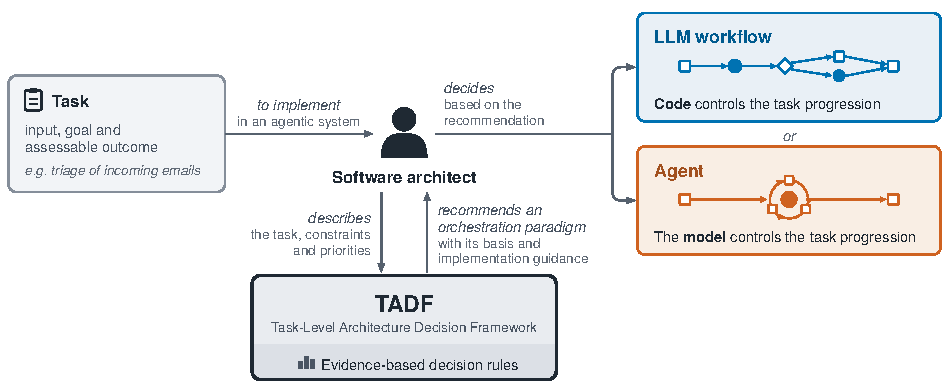
\includegraphics[width=\linewidth]{Figures/fig_tadf_scope (1).pdf}
\caption{Scope, functionality and context of the TADF.}
\label{fig:tadf-scope}
\end{figure}
 
The decision unit is a task: a bounded unit of work with an identifiable input, a coherent goal and an assessable outcome (Section~\ref{subsubsec:theory/task}). Before the comparison, TADF checks whether the task needs an LLM at all and whether it should be simplified or split into smaller tasks. This gives TADF four possible outcomes: deterministic implementation, decomposition, LLM workflow or agent. The coordination between tasks, the composition of several agents, the selection of an LLM and the operation of the deployed system lie outside its scope. The comparative evidence covers eight task archetypes, three OpenAI models and the implementations built for this thesis. TADF addresses the suitability of a model through implementation guidance, not through a model-selection procedure.
 
The research question is: (RQ) How can a task-level architecture decision framework be designed to support software architects in selecting between LLM workflows and agents for agentic workplace automation? Three sub-questions structure the answer: (SQ1) How do LLM workflows and agents compare in terms of task-relevant performance metrics across workplace tasks? (SQ2) Which task characteristics and execution conditions are associated with performance differences between LLM workflows and agents? (SQ3) How relevant is the distinction between LLM workflows and agents to architecture decisions in practice, and to what extent can the proposed framework support software architects in making these decisions? The research examines one hypothesis: A task-level architecture decision framework based on task characteristics provides consistent and practically useful recommendations for selecting between LLM workflows and agents in agentic workplace automation. This hypothesis is a design proposition, not a statistical hypothesis.
 
In design science research (DSR), the purpose of an artifact defines the goals that the artifact must meet \parencite{gregorPositioningPresentingDesign2013}. Section~\ref{subsec:TADF/objectives} derives eight design objectives from the purpose of TADF. They cover the decision core, decision quality and use and deployment. Consistency means that the same task characteristics, constraints and priorities lead to the same recommendation (O4). Practical usefulness has two parts. First, software architects find the recommendations relevant and can apply them with bounded effort (O2, O6, O7). Second, following the recommendations improves the trade-off between task success and token cost compared with using one orchestration paradigm for all tasks (O5). The first part concerns perceived usefulness, the second measured decision quality.
 
The thesis contributes to practice and to knowledge. For practice, TADF is a documented decision framework. It is delivered as a reusable set of instructions and reference documents for an LLM assistant. For knowledge, the thesis provides comparative evidence on both orchestration paradigms, based on a task taxonomy and paired implementations. The decision method of TADF and three design principles add design knowledge for decision support of this kind. Because practice currently addresses the problem with heuristics, the thesis aims at an improvement in the sense of \textcite{gregorPositioningPresentingDesign2013}: a better solution for a known problem.

\subsection{Research Method}
\label{subsec:intro/method}
The research question asks how an artifact should be designed. This thesis therefore follows DSR, in which knowledge about a problem and its solution is gained by building and applying an artifact \parencite{hevnerDesignScienceInformation2004}. A purely empirical comparison of the two orchestration paradigms could answer SQ1 and SQ2, but not the research question. A decision procedure must first be built, applied and revised before its value can be judged. In addition, DSR requires that the utility, quality and efficacy of an artifact be demonstrated through evaluation \parencite{hevnerDesignScienceInformation2004}. TADF is the artifact of this thesis. It is a framework that was first instantiated as a spreadsheet, the Decision Sheet, and later as the TADF skill framework. The paired implementations of both orchestration paradigms are not part of TADF, they provide its evidence.
 
The research follows the six activities of the design science research methodology (DSRM): problem identification and motivation, objectives of a solution, design and development, demonstration, evaluation and communication \parencite{article}. The entry point is problem-centered. The activities ran in iterations: results of the experiments and of each evaluation episode led to revisions of TADF. Such formative evaluation can be reported as part of the development \parencite{gregorPositioningPresentingDesign2013}. The demonstration is reported after the evaluation because it uses the version of TADF that resulted from both evaluation episodes. The three design principles were abstracted from these revisions and the evidence behind them, using the schema of \textcite{australiannationaluniversityaustraliaResearchPerspectivesAnatomy2020} (Section~\ref{subsec:discussion/contribution}).
 
In the three-cycle view of \textcite{hevnerThreeCycleView2007}, the iterative revisions form the design cycle. The rigor cycle and the relevance cycle link it to its context. The rigor cycle drew on a targeted literature review. It aimed to identify the concepts, theories and studies that the design of TADF requires, not to map the field completely. Keyword searches in Google Scholar, ScienceDirect and arXiv combined two groups of terms. The first described the systems, such as LLM workflow, agent, agentic workflow and multi-agent system. The second described the decision, such as orchestration, architecture decision and decision support. Backward snowballing from the included studies added further sources \parencite{wohlinGuidelinesSnowballingSystematic2014}. The searches were last updated in September 2026. Preprints were included because research on agentic systems moves faster than journal publication, and the bibliography records the version that was read. Documentation from AI providers and framework developers served only for definitions and practitioner guidance (Chapter~\ref{sec:theory}). In return, the comparative evidence and the design principles add to this knowledge base (Chapter~\ref{sec:discussion}). In the relevance cycle, reported practice motivated the problem. Practitioners assessed TADF once its initial version existed, and the demonstration applied the revised TADF to an external scenario. A field test in an organization was outside the scope.
 
SQ1 and SQ2 draw on one experimental program with two parts. The main experimental comparison implemented both orchestration paradigms for 120 task instances. The task instances cover eight task archetypes and were executed with three models (Sections~\ref{subsubsec:TADF/setup} to~\ref{subsubsec:TADF/results}). Both orchestration paradigms shared the task requirements, the sandbox and the measurement rules. Task success and token cost served as primary metrics, complemented by four secondary metrics. The implementations still differed in components and limits. The results are thus reported descriptively and do not isolate a causal effect of the orchestration paradigm. The main experimental comparison provides the evidence for SQ1. Because each task archetype has a profile on four task dimensions, it also provides first evidence for SQ2. Five deep-dive task families then varied selected task characteristics and execution conditions within one task archetype (Section~\ref{subsubsec:TADF/deepdive}). These exploratory runs address SQ2 more directly. The findings of both parts informed the gates and scoring rules of the initial TADF (Section~\ref{subsec:TADF/initial-artifact}).
 
SQ3 draws on two evaluation episodes, two pilot runs and a demonstration (Sections~\ref{subsec:TADF/evaluation} and~\ref{subsec:TADF/demonstration}). In Episode~1, twelve participants with experience in building agentic systems or automations with LLMs described their current decision practice and assessed the Decision Sheet. Ten took part in recorded interviews, and two answered in writing. In Episode~2, TADF gave recommendations for the 69 task templates of WorkBench in two separate passes. The routed execution of 690 task instances was then compared with using one orchestration paradigm for all tasks. The two pilot runs refined how TADF is delivered. The demonstration applied the revised TADF to an email-automation scenario and exposed limits in how reliably the LLM assistant follows the procedure. The evaluations used identified TADF versions, and later corrections are reported separately.
 
Each method answers a different question: the experiments examine execution, the interviews examine perceived relevance and requirements, and the pilot runs and the demonstration examine how the procedure is applied. In the evaluation framework of \textcite{venableFEDSFrameworkEvaluation2016}, the evaluation is mainly formative and artificial. Formative evaluation improves the artifact during its development, and artificial evaluation takes place in controlled settings instead of real use. The only summative element is the WorkBench comparison of routed and uniform choices, and it concerns the tested implementations. The interviews do not show unaided use or better decisions in practice. The analysis thus separates gains from better implementations from gains that result from the selection by TADF.
 
Two aspects of the method require transparency. First, in its skill form, TADF is executed by an LLM assistant. The recommendations in Episode~2 and the demonstration were produced by a model that followed frozen documents. Second, coding agents supported the construction of task instances and implementations. Reviews checked the task instances and implementations against the task requirements, the control distinction and the outcome checks (Section~\ref{subsubsec:TADF/paradigms}). The use of these tools is declared according to the examination rules. Appendix~\ref{app:protocol} documents the experimental protocol and its deviations. The accompanying repository contains the task instances, implementations, results and development log (Appendix~\ref{app:repository}). These records make the process traceable.

\subsection{Structure of this Thesis}
\label{subsec:intro/structure}
The six chapters follow the DSRM activities and the publication schema for DSR studies of \textcite{gregorPositioningPresentingDesign2013}. Chapter~\ref{sec:Background} lays the foundations. It defines agentic systems, the two orchestration paradigms and the task as the decision unit, introduces decision support and reviews related work. Chapter~\ref{sec:TADF/development} states the design objectives, reports the experiments and presents the initial TADF. It then reports the two evaluation episodes and the revisions they caused. Development and evaluation share one chapter because the evaluation was mainly formative. Chapter~\ref{sec:TADF/final} presents the final TADF, reports the demonstration and assesses the evidence against the design objectives. Chapter~\ref{sec:Discussion} answers the research questions, derives the design principles and discusses limitations and future research. Chapter~\ref{sec:Conclusion} concludes the thesis. The appendices and the accompanying repository document the procedures and evidence behind the claims.

% SEC2
\clearpage
\section{Theoretical Background}
\label{sec:Background}
Supporting the choice between an LLM workflow and an agent requires three foundations: clear concepts, knowledge of what decision support must provide, and an overview of existing research. This chapter establishes these foundations. Section~\ref{subsec:theory/agentic-systems} places the choice within agentic systems. Section~\ref{subsec:theory/workflows-agents} defines the two orchestration paradigms, the task as the decision unit and four task dimensions that later structure the experiments. Section~\ref{subsec:theory/decision-support} derives the basis for the design objectives. Section~\ref{subsec:theory/related-work} reviews related work and positions the TADF within it.

\subsection{Agentic Systems and Automatisation}
\label{subsec:theory/agentic-systems}
Agentic systems pursue complex goals with minimal human intervention \parencite{acharyaAgenticAIAutonomous2025}. Their basic building block is a LLM that is augmented with retrieval, tools and memory \parencite{schluntzBuildingEffectiveAI2024}. With these capabilities, agentic systems plan steps, use tools to gather information and act on other systems, and keep context across steps \parencite{dwivediAgenticAISystems2026,sapkotaAIAgentsVs2026}. The related terms AI agent, agentic AI and agentic system are often used interchangeably \parencite{hughesAIAgentsAgentic2025}. Following \textcite{hughesAIAgentsAgentic2025}, this thesis uses the term agentic system for an interconnected structure that performs a business function. The term agent refers to one of the two orchestration paradigms defined in Section~\ref{subsec:theory/workflows-agents}.

In IS research, agency is a matter of degree. \textcite{holldackAgenticInformationSystems2026} place agentic information systems on a continuum. It ranges from assisting systems that act under significant human guidance to autonomous systems that manage complex tasks with minimal human intervention. Business process management describes a similar continuum for process execution. Process management systems have long executed predefined process models. Agentic systems can also execute such models, but they can additionally generate process variations, make contextual decisions and adapt workflows during execution. Agentic process management systems must therefore support processes that range from human-driven to fully autonomous \parencite{dumasAgenticBusinessProcess2026}.

Within an agentic system, control is also allocated between predefined code and the model. The orchestration layer of such a system decomposes high-level tasks into subtasks and coordinates them according to predefined or adaptive execution policies. In LangChain, chains provide a deterministic task structure, whereas agents add adaptive decision-making \parencite{sapkotaLangChainVsLangGraph2025}. Workflow and agent patterns can be combined within one system \parencite{schluntzBuildingEffectiveAI2024}. Deployed systems show such combinations. In 16 of 20 production case studies, practitioners defined the sequence of tasks upfront instead of relying on open-ended planning  \parencite{panMeasuringAgentsProduction2025}. An analysis of more than 6,000 workflows on the low-code platform n8n points in the same direction. Model calls are commonly embedded in broader structures with control logic, and a smaller share of workflows uses agent components with tools 
\parencite{tangCharacterizingLargeLanguage2026}.

This thesis examines the allocation of control for single tasks and therefore separates two levels for agentic systems. In the email process of Section~\ref{subsec:intro/motivation}, triage, context gathering, draft composition and draft verification are separate tasks. At the system level, these tasks are coordinated: results pass from one task to the next, and the system determines which task follows. At the task level, each task is executed by a component that combines model calls, program logic and tools. Within this component, control over the progression of the task can lie with predefined code or with the model. The TADF addresses this task-level choice. 

\subsection{LLM Workflow vs. Agent}
\label{subsec:theory/workflows-agents}

The terms workflow and agent are used with different meanings. OpenAI uses workflow for the sequence of steps that must be executed to meet a user's goal, whether by conventional software or by an agent \parencite{openaiPracticalGuideAgents2026}. A survey of agent workflows uses the term for procedures in which several agents make a sequence of decisions \parencite{yuSurveyAgentWorkflow2025}. Anthropic and LangChain instead distinguish workflows from agents by who controls the execution path. In a workflow, model calls and tools are orchestrated through predefined code paths. In an agent, the model directs its own process and tool use \parencite{schluntzBuildingEffectiveAI2024,Workflowsandgents}. OpenAI draws the same line: an application counts as an agent only if the model controls the execution of the workflow \parencite{openaiPracticalGuideAgents2026}.

This thesis adopts this control-based distinction. An LLM workflow coordinates model calls and tools through a path structure that is predefined in code. The structure can contain branches, loops and routing by a model. An agent leaves control over the progression of the task to the model. Within limits set by the surrounding program, the model selects the next action \parencite{schluntzBuildingEffectiveAI2024,Workflowsandgents}. It also decides when the task is complete. This thesis calls the two alternatives orchestration paradigms, or paradigms for short. The distinction concerns control over the execution path. It does not depend on the use of tools, the number of model calls or the implementation framework.

\subsubsection{Building Blocks and Architectural Differences}
\label{subsubsec:theory/control}

Both orchestration paradigms use the same building blocks: bounded model operations, program logic and tool operations. They differ in which block controls the progression of the task. In an LLM workflow, program logic fixes the order of the model operations, the conditions for branching or repeating a stage and the checks applied to results. Each model operation returns a defined output for a defined input, such as an extracted field or a draft text. \textcite{schluntzBuildingEffectiveAI2024} describe five workflow patterns: prompt chaining, routing, parallelization, orchestrator-workers and evaluator-optimizer. In each pattern, code specifies the stages and the permitted transitions, even where a model selects a route or plans subtasks within a stage. DSPy formalizes this composition as modules with declared input and output signatures, which ordinary control flow connects \parencite{khattabDSPyCompilingDeclarative2023}.

In an agent, the model controls the steps. In ReAct, the model alternates reasoning with actions, and each action returns an observation that becomes part of the context for the next step \parencite{yaoReActSynergizingReasoning2023}. The surrounding program provides the permitted tools, executes the selected actions, returns their results and enforces limits such as a maximum number of iterations \parencite{schluntzBuildingEffectiveAI2024}. Actions need not call external tools. The Cognitive Architectures for Language Agents (CoALA) framework also counts internal actions, such as reasoning over the working memory \parencite{sumersCognitiveArchitecturesLanguage2024}. Deciding whether to revise a draft or to submit it is therefore also a model-selected action.

Other design choices are independent of this distinction. The same model, tool interfaces and memory are available to both paradigms. CoALA distinguishes working memory for the current task from long-term episodic and procedural memory \parencite{sumersCognitiveArchitecturesLanguage2024}. What a system retains is therefore a separate design question. The same holds for the number of agents and for the agent style, such as ReAct prompting or native function calling. AgentArch varies both as separate configuration dimensions \parencite{bogavelliAgentArchComprehensiveBenchmark2025}. None of these choices determines who controls the progression of a task. Table~\ref{tab:theory-workflow-agent} summarizes the differences that follow from the allocation of control.

\begin{table}[htbp]
  \centering
  \caption{Control of task progression in LLM workflows and agents.}
  \label{tab:theory-workflow-agent}
  \small
  \begin{tabular}{@{}>{\raggedright\arraybackslash}p{\dimexpr0.20\linewidth-\tabcolsep\relax} >{\raggedright\arraybackslash}p{\dimexpr0.40\linewidth-1.5\tabcolsep\relax} >{\raggedright\arraybackslash}p{\dimexpr0.40\linewidth-1.5\tabcolsep\relax}@{}}
    \toprule
    \textbf{Aspect} & \textbf{LLM workflow} & \textbf{Agent} \\
    \midrule
    Task progression & Code specifies the stages and the transitions between them. & The model selects actions from the evolving task state. \\
    \addlinespace[2pt]
    Model contribution & Bounded outputs and choices within the predefined path. & Outputs and decisions about how to continue. \\
    \addlinespace[2pt]
    Steps and tool calls & Follow the conditions of the predefined path. & Depend on the model, up to the limits of the program. \\
    \addlinespace[2pt]
    Adaptation & Branches, repetitions and recovery follow coded conditions. & The sequence can change in response to observations. \\
    \addlinespace[2pt]
    Completion & The coded path defines when the task is complete. & The model can decide that the task is complete. \\
    \addlinespace[2pt]
    Traceability & Paths and transitions are known in advance; the trace shows which were taken. & Objectives and limits are known in advance; the sequence appears only in the trace. \\
    \bottomrule
  \end{tabular}
\end{table}

\subsubsection{Task as the Unit of Decision}
\label{subsubsec:theory/task}

Both orchestration paradigms apply to the same unit: the task. In Business Process Model and Notation (BPMN), a task is an atomic activity that is not broken down further at the chosen level of process detail \parencite{BPMN}. Building on this notion, this thesis defines a task as the smallest bounded unit of work with an identifiable input, a coherent goal, an assessable outcome and an progression over paths activities or tools. A task may require several model calls or tool operations. The definition does not assume that a task needs an LLM. Whether deterministic code suffices is part of the decision (Section~\ref{subsec:TADF/initial-artifact}).

Four further units structure the analysis. A task instance specifies a concrete input, the relevant initial state and the acceptance conditions. A task archetype groups tasks with recurring structural requirements. An implementation realizes one orchestration paradigm for a task archetype. An execution applies an implementation to a task instance.

\subsubsection{Task Dimensions Relevant to the Choice}
\label{subsubsec:theory/importance}
Which orchestration paradigm fits depends on the task. Practitioner guidance recommends LLM workflows for well-defined tasks and agents for open-ended problems (Section~\ref{subsec:intro/problem}). It also recommends the simplest solution that works, which may mean not building an agentic system at all \parencite{schluntzBuildingEffectiveAI2024}. Research on related design options supports task-dependent selection (Section~\ref{subsec:theory/related-work}). No single reasoning strategy performs best across tasks \parencite{zhouSelectthenSolveParadigmRouting2026}, and the effect of multi-agent coordination depends on the structure of the task \parencite{kimScienceScalingAgent2025}.

The literature points to four task dimensions that are candidates for explaining performance differences between the paradigms and task fit. This thesis later uses them to describe and structure tasks for the experiments (Section~\ref{subsubsec:TADF/taxonomy}). (1) Step predictability describes how far the required steps can be specified before execution. LLM workflows follow predefined code paths, whereas agents select their actions during execution \parencite{schluntzBuildingEffectiveAI2024,yaoReActSynergizingReasoning2023}. Research on workflow optimization likewise distinguishes structures fixed before deployment from structures that are selected, generated or revised for a particular run \parencite{yueStaticTemplatesDynamic2026}. (2) Information availability describes whether the required information is supplied with the task, held in known stores or obtained through interaction with the environment. CoALA separates retrieval from long-term memory from actions that ground the agent in external environments \parencite{sumersCognitiveArchitecturesLanguage2024}. FlowBench studies workflow knowledge that is supplied to an agent in advance \parencite{xiaoFlowBenchRevisitingBenchmarking2024}. (3) Output ambiguity describes how precisely an acceptable result can be specified. Evaluation metrics range from exact match to programs that balance several concerns \parencite{khattabDSPyCompilingDeclarative2023}. Iterative refinement by an evaluator is particularly effective when clear evaluation criteria exist and refinement provides measurable value \parencite{schluntzBuildingEffectiveAI2024}. (4) Error consequence describes the potential impact of an incorrect result in the intended application. In workplace settings, an agent error can send an email to the wrong person \parencite{stylesWorkBenchBenchmarkDataset2024}. Tasks that follow domain policies require reliable and consistent changes to the system state \parencite{yao$t$benchBenchmarkToolAgentUser2024}.

\subsection{Architecture Decision Support}
\label{subsec:theory/decision-support}
Choosing an orchestration paradigm for a task is a semi-structured decision. Evidence can show how well each paradigm suits a task. The weight of the competing qualities, however, depends on the deployment and on the judgment of the software architect (Section~\ref{subsec:intro/problem}). Decision support systems (DSS) target such decisions. A DSS has three components: data about the problem, models that evaluate alternatives, and a dialogue through which users enter information and inspect results \parencite{spragueFrameworkDevelopmentDecision1980}. The following paragraphs first state the aim of decision support. They then describe what decision support needs to reach this aim and to be used in practice.

Above all, decision support must make decisions measurably better. Improving decision quality is the goal of every DSS \parencite{kasperTheoryDecisionSupport1996}. For software engineering, \textcite{ruheSoftwareDesicionsupport} states this goal as a hypothesis: decision support enables more effective decisions of improved quality. The confidence of users does not show whether this goal is reached. According to \textcite{kasperTheoryDecisionSupport1996}, confidence in a decision often differs from its objective quality, and overconfidence is common. He also reports studies in which decision aids raised the confidence of their users but not the quality of their decisions. The value of decision support must therefore be shown by measuring the quality of the resulting decisions. This requires relevant metrics \parencite{article} and a reference point, such as decisions made without the support \parencite{ruheSoftwareDesicionsupport}.

To reach this aim, decision support starts from an explicit decision space. Techniques for architecture decisions describe a decision by its alternatives and by the quality attributes that these alternatives fulfill. Each alternative fulfills an attribute to a certain level, and this level is uncertain \parencite{falessiDecisionmakingTechniquesSoftware2011}. In the choice studied here, the alternatives are the two orchestration paradigms. A complete decision space can also include other found alternatives, which may suffice for some tasks (Section~\ref{subsubsec:theory/importance}). The quality attributes, such as task success, token cost and predictability, also provide the metrics for decision quality. Some attributes must reach a minimum level, whereas for others more is simply better \parencite{falessiDecisionmakingTechniquesSoftware2011}. Constraints go further and directly include or exclude parts of an architecture \parencite{amellerLinkingQualityAttributes2012}. Constraints and minimum levels therefore decide which alternatives are feasible, and preferences rank the feasible ones. 

Which feasible alternative fits best depends on the task. Task-technology fit is the correspondence between task requirements, individual abilities and the functionality of a technology. Only a technology that fits the task can improve individual performance \parencite{goodhueTaskTechnologyFitIndividual1995}. For the choice studied here, different task dimensions, deployment constraints and user requirements are assessed. The two paradigms offer different kinds of fit to these task requirements. The comparison therefore asks which paradigm provides the control that the task needs. Because the choice is made before implementation, it must rest on task characteristics that a software architect can state in advance.

This comparison must rest on evidence. \textcite{ruheSoftwareDesicionsupport} observes that decisions in software engineering often do not rely on empirically evaluated models and are not explained to those involved. Decision support in software engineering responds by combining models, measurement, empirical studies and simulation to evaluate and select alternatives \parencite{ruheSoftwareDesicionsupport}. Such evidence holds only for the tasks, technologies and conditions it covers. A recommendation must therefore name its evidence, separate observed findings from assumptions, and state the conditions under which it applies. 

The reasoning behind a recommendation must also be traceable. \textcite{ruheSoftwareDesicionsupport} accordingly includes an explanation component that makes solution alternatives transparent. \textcite{gregorExplanationsIntelligentSystems1999} classify explanations by their content, and two types matter here. A trace explains a recommendation by the data and rules used in the case. A justification links the rules to the knowledge from which they were derived. Experts use explanations more than novices to verify a recommendation or to resolve a disagreement, and justifications should increase trust and acceptance \parencite{gregorExplanationsIntelligentSystems1999}. Such verification is harder for advice from AI-based systems, which are less transparent than rule-based systems and whose errors are less predictable \parencite{jussupowAugmentingMedicalDiagnosis2021}. This thesis also considers this for reproducibility. Recording the inputs, the applied rules and their version ensures that the same inputs yield the same recommendation under the same version.

Decision support also extends to acting on a decision. \textcite{spragueFrameworkDevelopmentDecision1980} counts implementation among the phases of decision making that a DSS should support. For an orchestration paradigm, acting on a recommendation means building the LLM workflow or the agent. Recommendations therefore need guidance on how to implement the chosen paradigm. 

Finally, decision support helps only if professionals use it in their daily work. Fit with the task is not enough, because a technology improves individual performance only if it is also used \parencite{goodhueTaskTechnologyFitIndividual1995}. Users of a DSS can often decide for themselves whether to use it, so ease of use is particularly important \parencite{spragueFrameworkDevelopmentDecision1980}. According to \textcite{gregorExplanationsIntelligentSystems1999}, users read explanations only if the expected benefit outweighs the mental effort, and explanations requiring less effort are used more. They also point out that learning decisions and working constantly compete at work \parencite{lebovitzEngageNotEngage2022,gregorExplanationsIntelligentSystems1999}. Recommendations and implementation guidance must therefore be understandable for software architects and applicable with bounded effort. Together, these foundations describe what decision support for the choice of an orchestration paradigm must provide. Section~\ref{subsec:TADF/objectives} derives the design objectives of TADF from them.

\subsection{Related Work}
\label{subsec:theory/related-work}
Related research covers parts of the task-level choice. This section draws on the targeted review described in Section~\ref{subsec:intro/method}. It groups the studies into five streams. These streams differ in what they select, when they select it and on which evidence. Direct comparisons test both paradigms but offer no method for choosing between them. Studies of configurations select among agent designs only. Run-time methods select among implemented strategies, design guidance remains qualitative, and workplace benchmarks evaluate agents without a paired LLM workflow. No reviewed approach offers an evidence-based method for choosing between code control and model control for a single task before implementation.
 
The first stream is closest to the choice studied here. Two studies compare code control and model control directly. SourceCodeAgent follows the principle ``Blueprint First, Model Second''. An expert-defined procedure is written as code and run by a deterministic engine, while the LLM handles bounded subtasks but never decides the path \parencite{qiuBlueprintFirstModel2025}. Under the definitions of Section~\ref{subsec:theory/workflows-agents}, this is an LLM workflow. On the TravelPlanner benchmark with Claude Sonnet~4, it reached a final pass rate of 35.56\%, against 18.00\% for the multi-agent system ATLAS. The authors attribute the advantage to deterministic enforcement rather than a richer specification. On the explicit constraints of the user, however, the workflow performed comparably and produced more violations. They conclude that the payoff of code control scales with how procedurally well-defined and constraint-intensive a task is. For open-ended tasks, they consider general-purpose agents more suitable. \textcite{dennisInContextPromptingObsoletes2026} report the opposite for procedural dialogues. A complete procedure in the system prompt, followed by the model itself, reached higher judged quality than a LangGraph orchestrator with the same model. This held across three domains, but the prompted approach used more tokens. Both studies concern tasks with a defined procedure, yet they favor different paradigms. They differ in the kind of task and in what they measure. A defined procedure alone therefore does not settle the choice, and neither study offers a method for choosing a paradigm for a given task.
 
The second stream supports choosing the architecture for each task. It shows that the architecture of an agentic system affects its performance and that no single design fits every task and model. AgentArch evaluates 18 configurations on two enterprise use cases. They vary single-agent and multi-agent orchestration, ReAct and function calling, memory and thinking tools. The best configuration differs by model and task, which challenges one-size-fits-all designs \parencite{bogavelliAgentArchComprehensiveBenchmark2025}. \textcite{kimScienceScalingAgent2025} underline this and compare a single agent with four multi-agent architectures across 260 configurations, three model families and six benchmarks. Compared with the single agent, performance rose by up to 80.8\% on decomposable reasoning and fell by up to 70.0\% on sequential planning. The authors attribute the benefit of coordination to measurable task properties such as decomposability rather than to the number of agents. \textcite{gaoSingleagentMultiagentSystems2025} find that the accuracy advantage of multi-agent systems narrows as models improve and that simple tasks can suffer from overthinking. These studies compare configurations of agents, however, not code control with model control.
 
The third stream shows that selection pays off: choosing an execution strategy for each input can improve accuracy and reduce cost. \textcite{gaoSingleagentMultiagentSystems2025} route requests between single-agent and multi-agent systems. An LLM rater compares the difficulty of a request with a threshold. A cascade instead escalates a request only when the single-agent result fails a check. They report accuracy gains of 1.1 to 12\% at lower cost. Difficulty-Aware Agentic Orchestration (DAAO) starts from the observation that workflows fixed for a whole task over-process simple queries or underperform on complex ones. It estimates the difficulty of each query and composes a workflow from operators such as chain-of-thought, debate, review, ReAct and testing. DAAO reports up to 11.21\% higher accuracy at up to 36\% lower cost \parencite{suDifficultyAwareAgenticOrchestration2025}. Select-then-Solve compares six reasoning strategies across four models and ten benchmarks \parencite{zhouSelectthenSolveParadigmRouting2026}. A learned router reaches 53.1\% average accuracy, against 50.3\% for the best fixed strategy. Letting a model choose its own strategy helped only the strongest model, which still trailed the learned router. Select-Then-Decompose and LLM-as-Scheduler likewise choose or adapt strategies for each input, the latter with risk-tiered thresholds \parencite{liuSelectThenDecomposeEmpiricalAnalysis2025,xiangLLMasSchedulerAgenticWorkflow2026}. These approaches work during operation and choose among strategies that are already implemented, and learned routers need execution data for training. A software architect, in contrast, must decide before implementation which paradigm to build.
 
The fourth stream offers guidance for the same kind of design decision as this thesis. Besides the practitioner guidance discussed in Section~\ref{subsubsec:theory/importance}, the Agent Design Pattern Catalogue describes 18 architectural patterns with their context, forces and trade-offs. It proposes a decision model for selecting them and rests on a systematic literature review \parencite{liuAgentDesignPattern2025}. Its patterns concern how agents pursue goals and generate plans, not whether code or the model should control a task. In a survey of workflow optimization, \textcite{yueStaticTemplatesDynamic2026} recommend starting from a constrained static structure and adding flexibility only where the workload requires it. They reserve changes during execution for settings in which partial execution reveals information that a plan made in advance cannot anticipate. They call this recipe not universal. In their view, the field lacks a clear theory of when dynamic workflow generation is necessary and when static templates suffice. This guidance is qualitative and does not assess a given task against paired executions of both paradigms.
 
The fifth stream provides the realistic tasks and outcome checks on which evidence for the choice can be built. Benchmarks cover common business activities such as sending emails and scheduling meetings \parencite{stylesWorkBenchBenchmarkDataset2024}, realistic workflows of knowledge workers \parencite{boisvertWorkArenaCompositionalPlanning2025} and tasks in customer relationship management \parencite{huangCRMArenaProHolisticAssessment2025}. WorkBench counts a task as solved when the outcome of the actions matches a unique ground-truth outcome \parencite{stylesWorkBenchBenchmarkDataset2024}. $\tau$-bench likewise compares the final database state with an annotated goal state and adds dialogues with simulated users under domain policies. Even the strongest function-calling agent averaged a success rate below 50\% across its two domains and was inconsistent across repeated trials \parencite{yao$t$benchBenchmarkToolAgentUser2024}. The most competitive agent completed 30\% of the tasks in TheAgentCompany \parencite{xuTheAgentCompanyBenchmarkingLLM2025}. World of Workflows adds hidden workflows in enterprise systems whose effects cascade across connected databases \parencite{guptaWorldWorkflowsBenchmark2026}. On CRMArena-Pro, workflow execution was notably more tractable than the other business skills, with top agents exceeding 83\% success in single-turn tasks \parencite{huangCRMArenaProHolisticAssessment2025}. These benchmarks evaluate agents without a paired LLM workflow. FlowBench comes closest to a comparison with predefined control, but it varies only whether and in which format workflow knowledge is given to ReAct agents \parencite{xiaoFlowBenchRevisitingBenchmarking2024}. Section~\ref{subsubsec:TADF/taxonomy} uses these benchmarks as sources for the task archetypes of the experiments.
% SEC 3
\clearpage
\section{Design, Development and Evaluation}
\label{sec:TADF/development}
Turning the foundations of Chapter~\ref{sec:Background} into decision support takes four steps: objectives, evidence, design and evaluation. This chapter reports these steps for the TADF.  Section~\ref{subsec:TADF/objectives} derives eight design objectives. Section~\ref{subsec:TADF/design} reports the experimental program that compared both orchestration paradigms on the same tasks. Section~\ref{subsec:TADF/initial-artifact} presents the initial framework, the Decision Sheet, and shows how this evidence shaped its gates and scoring rules. Section~\ref{subsec:TADF/evaluation} reports two evaluation episodes: practitioner interviews and a WorkBench evaluation. It also describes the revisions they caused and two pilot runs of the revised framework. Because they were highly formative, they are reported together with the design and devleopment \parencite{gregorPositioningPresentingDesign2013}.

\subsection{Design Objectives for the Framework}
\label{subsec:TADF/objectives}
The overall objective of TADF is to support software architects in choosing an orchestration paradigm for single tasks before implementation (Section~\ref{subsec:intro/scope}). Eight design objectives specify this purpose. Following the second DSRM activity, they are inferred from the problem definition (Section~\ref{subsec:intro/problem}) and from knowledge of what is possible and feasible \parencite{peffersDesignScienceResearch2007}. They state what TADF must achieve, and later results are assessed against them \parencite{gregorPositioningPresentingDesign2013}.

According to Section~\ref{subsec:theory/decision-support}, decision support starts from an explicit decision space: constraints and minimum levels decide feasibility, and preferences rank the feasible alternatives. TADF must therefore cover the relevant alternatives (Section~\ref{subsubsec:theory/importance}), and the conditions under which each applies (O1). Since the fit depends on the task and the choice precedes implementation, recommendations must rest on structural task characteristics known in advance (O2). Because existing guidance is qualitative and lacks paired evidence (Section~\ref{subsec:theory/related-work}), each recommendation must name its empirical evidence and separate observed findings from assumptions (O3).

Decision quality requires traceable reasoning and, above all, measurable improvement (Section~\ref{subsec:theory/decision-support}). Identical task characteristics, constraints and priorities must yield the same recommendation under the same version, and its reasoning must be reconstructible (O4). User confidence does not show decision quality. Recommended choices must therefore improve the trade-off between task success and token cost over a uniform choice of one paradigm for all tasks (O5). This reference point uses no task-level support.

Because acting on a recommendation means building the LLM workflow or the agent (Section~\ref{subsec:theory/decision-support}), each recommendation must include task-specific implementation knowledge (O6). Since decision support helps only if it is used in daily work, TADF must be understandable for software architects and applicable with bounded effort (O7). Because evidence holds only for the tasks, technologies and conditions it covers, TADF must rest on realistic workplace tasks and declare its scope (O8). Table~\ref{tab:design-objectives} lists the objectives across three categories and their basis.

\begin{table}[htbp]
  \centering
  \caption{Design objectives for the TADF.}
  \label{tab:design-objectives}
  \small
  \begin{tabular}{@{}l l >{\raggedright\arraybackslash}p{7.5cm} l@{}}
    \toprule
    \textbf{ID} & \textbf{Category} & \textbf{Objective} & \textbf{Basis} \\
    \midrule
    O1 & Decision core & Complete and structured decision space & \ref{subsubsec:theory/importance}, \ref{subsec:theory/decision-support} \\
    O2 & Decision core & Decisions based on task characteristics & \ref{subsubsec:theory/importance}, \ref{subsec:theory/decision-support} \\
    O3 & Decision core & Decisions grounded in empirical evidence & \ref{subsec:intro/problem}, \ref{subsec:theory/decision-support}, \ref{subsec:theory/related-work} \\
    O4 & Decision quality & Reproducible and traceable decisions & \ref{subsec:theory/decision-support} \\
    O5 & Decision quality & Measurably better architecture decisions & \ref{subsec:intro/problem}, \ref{subsec:theory/decision-support} \\
    O6 & Use \& deployment & Clear decisions with implementation knowledge & \ref{subsec:intro/problem}, \ref{subsec:theory/decision-support} \\
    O7 & Use \& deployment & Usability with bounded effort & \ref{subsec:theory/decision-support} \\
    O8 & Use \& deployment & Grounding in workplace tasks and with a scope & \ref{subsec:intro/scope}, \ref{subsec:theory/decision-support}, \ref{subsec:theory/related-work} \\
    \bottomrule
  \end{tabular}
\end{table}

\subsection{Design and Development}
\label{subsec:TADF/design}
This section reports the experimental program that provides the empirical basis of the TADF. It supplies the evidence for SQ1 and SQ2 and for the objectives on task characteristics, empirical grounding and realistic tasks (O2, O3, O8). A task taxonomy defines which tasks are compared (Section~\ref{subsubsec:TADF/taxonomy}). A shared sandbox and fixed measurement rules form the experimental setup (Section~\ref{subsubsec:TADF/setup}). Both orchestration paradigms are implemented, validated and executed on the same task instances (Section~\ref{subsubsec:TADF/paradigms}). Deep-dive runs examine questions that the main experimental comparison left open (Section~\ref{subsubsec:TADF/deepdive}). Section~\ref{subsubsec:TADF/results} reports the results that inform the initial framework in Section~\ref{subsec:TADF/initial-artifact}. The repository contains the task instances, implementations and development log (Appendix~\ref{app:repository}).

\subsubsection{Task Taxonomy}
\label{subsubsec:TADF/taxonomy}
The main experimental comparison needs a defined set of tasks. Its results must reveal a performance to task characteristic connection so that software architects can use this to make a decision before implementation (O2). They must also rest on realistic workplace tasks (O8). In addition, the set must cover tasks that differ in execution. Tasks with tools need information from other systems or change their state. Input-only tasks are solved from input that already contains all required information. The choice between the orchestration paradigms arises for both, because their distinction does not depend on tool use (Section~\ref{subsec:theory/workflows-agents}). A set limited to one of them could favor one paradigm in advance.

Existing benchmark sources provide realistic tasks, but they group them mainly by domain or task type (Table~\ref{tab:corpus-positioning}). Three group tasks by a single structural characteristic, such as the number of applications. None groups them by a profile of structural characteristics that bear on the choice between the orchestration paradigms. Most also contain only tasks with tools. A task taxonomy was therefore developed for this study. It consists of four task dimensions that span the task space and eight task archetypes that represent recurring task patterns within it.

The development adapted the taxonomy method of \textcite{nickersonMethodTaxonomyDevelopment2013}, which combines conceptual-to-empirical and empirical-to-conceptual iterations. The meta-\hspace{0pt}characteristic comprises the task requirements that bear on who should control the progression of a task (Section~\ref{subsec:theory/workflows-agents}). It is the basis for choosing the dimensions and their values \parencite[p.~343]{nickersonMethodTaxonomyDevelopment2013}. Four task dimensions were first derived conceptually from the literature: step predictability, information availability, output ambiguity and error consequence (Section~\ref{subsubsec:theory/importance}). Tasks from benchmark sources were then mapped to these dimensions and grouped into task archetypes by their dimensional profiles and defining results. The review of benchmark sources ended when an additional source yielded no new task archetype and required no change to the dimensions or their values. This stopping rule corresponds to two objective ending conditions of the method \parencite[p.~344]{nickersonMethodTaxonomyDevelopment2013}. During the build-up of the experiments, the dimension values received explicit definitions and several profiles were adjusted for better distinction. The taxonomy was fixed before the final runs of the main experimental comparison, and the set of eight task archetypes remained the same throughout (Appendix~\ref{app:taxonomy/development}).

Benchmark sources came from the literature review (Section~\ref{subsec:intro/method}) and from backward snowballing through their references \parencite{wohlinGuidelinesSnowballingSystematic2014}. The task defined in Section~\ref{subsubsec:theory/task} was the unit of analysis, and longer scenarios entered through their constituent tasks. A benchmark source was included if it specified tasks at this level and contributed task patterns relevant to workplace or enterprise automation. Exclusion criteria covered abstract capability tests, isolated environment interaction, consumer or social contexts, incompatible units of analysis and patterns already represented (Appendix~\ref{app:taxonomy/corpus}). Of 48 benchmark sources, 13 were included (Table~\ref{tab:corpus-positioning}) and 35 were excluded (Appendix~\ref{app:taxonomy/exclusions}). Appendix~\ref{app:taxonomy/sources} links each included source to the task archetypes it informed. The ending condition concerns stability within this task space and does not establish exhaustive coverage of workplace tasks.

\begin{table}[htbp]
  \centering
  \caption[Included benchmark sources compared with this study.]{Included benchmark sources compared with the task taxonomy of this study. Tasks with tools need information from other systems or change their state; input-only tasks are solved from input that already contains all required information. Grouping by domain covers domains, platforms, websites, business scenarios, job roles and topics. Grouping by task type covers kinds of work and skills. Grouping by structure uses a profile of structural task characteristics. Difficulty levels are explicit levels assigned to the tasks.}
  \label{tab:corpus-positioning}
  \footnotesize
  \setlength{\tabcolsep}{4pt}
  \begin{tabular}{@{}>{\raggedright\arraybackslash}p{\dimexpr\linewidth-9cm-12\tabcolsep\relax} >{\centering\arraybackslash}p{1.4cm} >{\centering\arraybackslash}p{1.4cm} >{\centering\arraybackslash}p{1.4cm} >{\centering\arraybackslash}p{1.4cm} >{\centering\arraybackslash}p{1.7cm} >{\centering\arraybackslash}p{1.7cm}@{}}
    \toprule
     & \multicolumn{2}{c}{\textbf{Tasks}} & \multicolumn{3}{c}{\textbf{Grouping of tasks by}} & \textbf{Difficulty} \\
    \cmidrule(lr){2-3}\cmidrule(lr){4-6}
    \textbf{Benchmark source} & \textbf{with tools} & \textbf{input only} & \textbf{domain} & \textbf{task type} & \textbf{structure} & \textbf{levels} \\
    \midrule
    WorkBench  & \cmark & \xmark & \cmark & \xmark & (\cmark) & \xmark \\
    WONDERBREAD & \xmark & \cmark & \xmark & \cmark & \xmark & \cmark \\
    World of Workflows & \cmark & \cmark & \xmark & \cmark & \xmark & \xmark \\
    WorkArena++ & \cmark & \xmark & \xmark & \cmark & (\cmark) & \cmark \\
    TheAgentCompany  & \cmark & \xmark & \cmark & \xmark & \xmark & \xmark \\
    OfficeBench  & \cmark & \xmark & \xmark & \xmark & (\cmark) & \cmark \\
    CRMArena-Pro  & \cmark & \xmark & \cmark & \cmark & \xmark & \xmark \\
    \textcite{kouraniEvaluatingLargeLanguage2024} & \xmark & \cmark & \xmark & \xmark & \xmark & \xmark \\
    WebArena & \cmark & \xmark & \cmark & \cmark & \xmark & \xmark \\
    AssistantBench & \cmark & \xmark & \xmark & \xmark & \xmark & \cmark \\
    BrowseComp & \cmark & \xmark & \cmark & \xmark & \xmark & \xmark \\
    FlowBench & \cmark & \xmark & \cmark & \xmark & \xmark & \xmark \\
    $\tau$-bench & \cmark & \xmark & \cmark & \xmark & \xmark & \xmark \\
    \midrule
    \textbf{This study} & \cmark & \cmark & \xmark & \cmark & \cmark & \cmark \\
    \bottomrule
  \end{tabular}
\end{table}

The resulting eight task archetypes are defined as follows. (A) Exploratory research and synthesis. These tasks require locating relevant sources through search and combining the information found into a factual answer. (B) Structured data retrieval and transformation. These tasks require retrieving data from one or more known systems and combining or reformatting it as needed to produce the requested output. (C) Ambiguous classification and disambiguation. These tasks require assigning each input to a predefined category by interpreting its meaning, including cases with unclear or competing signals. (D) Compliance and rule-based decisioning. These tasks require applying explicit policy rules to case facts to determine the required decision, such as approval or rejection. (E) Output verification and quality control. These tasks require checking an existing output against stated criteria and returning a verdict, such as pass or fail. (F) Transactional action execution. These tasks require carrying out actions that change a system's state, such as updating records or sending messages. Later actions may depend on the results of earlier actions. (G) Strategic and adaptive planning. These tasks require selecting and ordering actions to reach a specified goal while respecting the conditions for each action. The result is a plan for later execution. (H) Content drafting and refinement. These tasks require drafting text from supplied information while meeting content and presentation requirements. When feedback is provided, the draft must be revised accordingly.

Below, the task archetypes are referred to by their letters A--H. Each task archetype has a distinct profile on the four task dimensions. Where profiles overlap, explicit assignment rules separate neighboring task archetypes (Appendix~\ref{app:taxonomy/dimensions}). A single coder assigned the benchmark tasks and profiles, so agreement between coders was not assessed. For the experiments, each task archetype received its own difficulty axis with the levels low, medium and high (Appendix~\ref{app:taxonomy/difficulty}). Examples are the number and dependence of information sources in A and the number of systems to combine in B. The main experimental comparison can thus examine changes in performance within each task archetype.

\subsubsection{Experimental Setup}
\label{subsubsec:TADF/setup}
The experimental setup turns the task taxonomy into a paired comparison of LLM workflows and agents. It defines three elements: the rules for the executions, the sandbox environment with its tools, and the metrics with their measurement.

The execution rules keep each pair comparable. Each task archetype has one LLM workflow and one agent. Both process the same task instances, 120 in total, with the same model, model settings and tools, and the same rules measure their results. The pair is thus designed to differ in the control over the progression of the task, which separates the orchestration paradigms (Section~\ref{subsubsec:theory/control}). One run of an implementation on a task instance with a model is an execution (Section~\ref{subsubsec:theory/task}). An experimental protocol, written before the implementation, specified this design, the metrics and the analysis. Appendix~\ref{app:protocol/changes} compares it with the implemented procedure. Section~\ref{subsubsec:TADF/paradigms} describes how each pair realizes the design.

The sandbox holds synthetic CRM, mail and calendar records in a local SQLite database and policy texts in a separate registry. Fifteen tool functions give access to these services and to web search (Table~\ref{tab:tools}). Because real services respond with a delay, most tool calls wait 250 to 350 milliseconds. The delay is derived from the call itself, so identical calls wait equally long in both orchestration paradigms. Web search stores its results per query, so identical queries also return identical results (Appendix~\ref{app:protocol/environment}).

Task success and token cost are the primary metrics, because O5 requires recommendations that improve the trade-off between them. The routing value of TADF is later measured with the same metrics (Sections~\ref{subsubsec:TADF/functionality} and~\ref{subsubsec:TADF/episode2}). Task success checks whether the result meets the acceptance conditions of the task instance, regardless of the path to it, as in the outcome-based evaluation of WorkBench \parencite{stylesWorkBenchBenchmarkDataset2024}. For B--G, deterministic checks compare the answer, labels, decision, verdict, system state or simulated plan outcome with the reference. For H, deterministic checks of content, length, structure, numbers and feedback decide success. Token cost is the sum of provider-reported input and output tokens over all model calls of an execution (Appendix~\ref{app:protocol/metrics}).

For two task archetypes, fixed rules cannot make the whole judgment. In A, a correct answer may differ from the reference in wording, units or rounding. In H, rules cannot fully capture writing quality. Both therefore use an LLM judge, a model that rates an output against given criteria. In A, its decision whether the answer states the reference fact is the task success. In H, it rates five criteria, such as completeness and conciseness, from 1 to 5. The judge sees the task, the reference or the criteria and one output, but not the orchestration paradigm. It uses a fixed prompt at temperature 0 and runs on the model of the assessed execution. LLM judges can favor longer answers or outputs of their own model \parencite{zhengJudgingLLMasaJudgeMTBench2023}. Their ratings were therefore compared with human ratings of six anonymized development outputs each for A and H. For A, judge and human agreed on all six. For H, agreement stayed below the planned threshold, so H's quality score only complements task success (Appendix~\ref{app:protocol/judges}).

Four secondary metrics describe further properties that matter in operation. Latency is the elapsed time of an execution, summarized by its median. Error rate is the share of executions that end with an error or exceed their step limit. Tool-call count is the number of tool calls in an execution. Robustness is the success rate on 42 variants of task instances whose wording was changed, for example by typos, jargon or irrelevant details, while their references stayed the same.

\subsubsection{Implementation and Execution}
\label{subsubsec:TADF/paradigms}
This section describes how the experimental setup was realized: the task instances, the implementations of both orchestration paradigms, their development and the execution of the main experimental comparison. Appendices~\ref{app:protocol/implementation} to~\ref{app:protocol/execution} and the repository (Appendix~\ref{app:repository}) document the details.

Fifteen task instances were constructed for each task archetype, five per difficulty level, with the help of coding agents. They transfer the task patterns of the benchmark sources to the local data and tools and are not copies of published tasks (Appendix~\ref{app:taxonomy/sources}). Where no source offered a suitable pattern, instances were designed for a specific requirement, for example five F instances whose actions depend on earlier results.

All implementations use Python with LangGraph and LangChain and call the models through the OpenAI API. Each LLM workflow is a graph with fixed edges: code sets the order of the stages and processes the structured outputs of the model calls. The agents of A to G use the prebuilt ReAct agent of LangGraph. In each step, the model either requests tool calls, whose results return to it, or gives its final answer \parencite{yaoReActSynergizingReasoning2023}. The agent of H has no tools. After each draft, its model decides whether to revise it again or to submit it. Figures~\ref{fig:paradigms-agents} and~\ref{fig:paradigms-workflows} show both control flows.

Within each pair, the task instance, the model and its settings, the available tools and the measurement are identical. By design, the pair differs in the control over the progression of the task. The deterministic components of the LLM workflows, such as the SQL processing in B, belong to this difference. Three further differences result from the implementation. The LLM workflow of A runs at most ten searches, while its agent made eleven and fifteen searches in two executions despite its step limit. From its second model call on, the agent of H no longer receives the table and the constraints, which each revision of the LLM workflow receives again. Finally, the step limits of the agents differ between task archetypes (Table~\ref{tab:app-implementations}).

\emph{(A) Exploratory research and synthesis.} The task instances ask research questions that require independent searches or linked searches, in which one finding determines the next query. The LLM workflow plans all queries first, runs up to ten searches and then synthesizes the answer. The agent chooses each search from the results so far. Both use only web search.

\emph{(B) Structured data retrieval and transformation.} The task instances ask for information from the CRM, mail and calendar systems. The LLM workflow specifies searches and SQL queries, fetches the records, combines them through read-only SQL and formulates the answer. The agent retrieves records step by step and combines them in its context. Both use the CRM read and search tools and the mail and calendar search tools.

\emph{(C) Ambiguous classification and disambiguation.} The task instances contain batches of three, five or eight support emails and five category definitions. The LLM workflow splits a batch into groups of at most five and classifies each group in one model call. The agent classifies the whole batch in one context. The available CRM tools are not needed.

\emph{(D) Compliance and rule-based decisioning.} The task instances contain quote requests that must be approved, refused or escalated under rules in a separate policy registry. The LLM workflow retrieves all policies, extracts the request facts in one model call and lets a rule engine decide. The agent retrieves the policies it needs and applies them in its context. The available CRM tools are irrelevant.

\emph{(E) Output verification and quality control.} The task instances pair a customer inquiry and a candidate response with a rubric of five criteria. The LLM workflow assesses the criteria in one model call, and code derives the verdict from the number of failed criteria. The agent assesses the response and derives the verdict in its context. The available CRM tools are not needed.

\emph{(F) Transactional action execution.} The task instances request changes to CRM, mail or calendar records, and the database is restored before each execution. The LLM workflow plans and runs reads, then plans the actions and executes them in order without revising the list. The agent can alternate reads and actions based on returned results. Both have access to all twelve CRM, mail and calendar tools.

\emph{(G) Strategic and adaptive planning.} The task instances set CRM goals that require a plan of actions, which a simulator checks afterwards. The LLM workflow plans and runs reads and then generates the complete plan. The agent can request further records before it returns its plan. Both use only the CRM read and search tools and execute no action.

\emph{(H) Content drafting and refinement.} The task instances combine a data table, writing constraints and a brief with zero to two scripted feedback rounds. The LLM workflow writes a draft and revises it once per feedback round. The agent decides after each draft whether to revise it again or to submit it, and a submission releases the next feedback round. Neither uses tools.

Task instances and implementations were developed in alternating build and test steps, following the design cycle of DSR \parencite[p.~90]{hevnerThreeCycleView2007}. Reviews checked each pair against the task requirements, the control distinction and the outcome checks. Observed failures led to changes, for example a read stage before action planning in F and a separate policy registry in D (Appendix~\ref{app:protocol/development}). The implementations were then frozen for the main experimental comparison. Because development results shaped them, the comparison provides formative evidence on a development corpus, not a test on unseen tasks.

The main experimental comparison ran on 6 and 7 July 2026 with GPT-5.4-nano, GPT-5.4-mini and GPT-5.2. The three models show whether differences between the orchestration paradigms persist across models, but they do not establish independence from the model. GPT-5.4-nano and GPT-5.4-mini ran two clean repetitions and GPT-5.2 one, and each model processed the 42 perturbation variants once per orchestration paradigm. This gives 1,200 clean and 252 perturbation executions. Seven batches of A were repeated after a usage limit of the search provider (Appendix~\ref{app:protocol/execution}).

Despite temperature 0 and a fixed seed, task success changed between the two clean repetitions in 49 of 480 matched combinations of task instance, orchestration paradigm and model (10.2 percent). Repetitions thus stabilize estimates for the same task instances but do not add tasks. The results concern the implemented systems; a failure of one implementation does not show that its orchestration paradigm is unsuitable in general. These results informed the initial framework (Section~\ref{subsec:TADF/initial-artifact}) and the deep-dive runs introduced next.

\subsubsection{Deep-Dive Task Runs}
\label{subsubsec:TADF/deepdive}
The main experimental comparison showed where the orchestration paradigms differed, but not always why. Within a task archetype, several task characteristics varied together. In F, for example, the high difficulty level combined aggregation, action sequences and actions that depend on earlier results (Appendix~\ref{app:taxonomy/difficulty}). The first routing questions derived from these results, TADF v1, therefore left open which characteristics should decide (Section~\ref{subsubsec:TADF/evolution}). The deep-dive runs examined these questions and thus address SQ2 more directly. They were designed after the main experimental comparison and were not part of the experimental protocol (Appendix~\ref{app:protocol/changes}), so they are exploratory.

Five task families each varied one characteristic or a combination of two within F, whose tasks change the system state and receive tool outcomes. P (plan uncertainty) varied what is unknown at the start. In its variants, a read or earlier action outcomes determine the number of actions, a needed fact lies in one of three systems that the task does not name, or record values determine the order. X (crossed gates) combined two characteristics that TADF v1 addressed in separate questions, such as written rules applied to action outcomes. L (payload scaling) multiplied the number of records by five and twenty to separate effects on task success from effects on token cost. M (state drift) changed a record during the execution: observably, silently, or silently with an instruction to re-check records. S (staged adaptivity) examined whether an LLM workflow can handle outcome-dependent tasks if code selects predefined branches after each tool outcome. Five of its task instances also require a report on the completed actions.

P, X, L and M reused the LLM workflow and the agent of F unchanged, and S added its state-machine LLM workflow as implementation. All families used the three models and repetitions of the main experimental comparison. Each execution started from the restored database, extended by additional records in L and by a trigger that changes a record in M. Task success and token cost were measured as in F. The runs comprise 73 new task instances and 805 executions (Appendix~\ref{app:protocol/deepdive}).

A confirmation test examined a map-form LLM workflow, which plans each item of a task in a separate model call instead of all actions in one. It was meant to supply the LLM-workflow side of a Decision Sheet criterion for item-specific values (Section~\ref{subsubsec:TADF/evidence}). Its target was an F instance on which the original LLM workflow had failed in three of five executions: reassigning the nine cases of one agent to another agent. Because all nine records receive the same value, the test did not measure item-specific values. An F instance with sixteen stage changes served as the control (Appendix~\ref{app:results/contrasts}). The test used GPT-5.2 in two repetitions.

The development log states hypotheses in advance only for S and the confirmation test. During the runs, one scoring error and two errors in shared tools were found and corrected for both orchestration paradigms. Section~\ref{subsubsec:TADF/results} reports the results as formative evidence on constructed task instances and the tested implementations.

\subsubsection{Results}
\label{subsubsec:TADF/results}
This section reports the results of the main experimental comparison and the deep-dive runs, which form the evidence base of the framework. They describe the implemented systems on the constructed task instances. Repeated executions of a task instance are not independent, so intervals and tests treat the task instance as the unit. Appendix~\ref{app:results} contains the detailed tables, and the repository the used code for analysing the results. 

\paragraph{Main experimental comparison.}
Table~\ref{tab:grid-results} reports task success, token cost, latency, tool calls and error rate for the 1,200 executions on the original task instances. Three success differences are clear, because their 95 percent intervals exclude zero. The LLM workflow was more successful in compliance (D), by 20.0 percentage points (interval 9.3 to 32.0), and in drafting (H), by 14.7 (5.3 to 26.7). The agent was more successful in action execution (F), by 26.7 (8.0 to 48.0). The agent was also more successful in research, retrieval and planning (A, B, G), but these intervals include zero, as do those of classification and verification (C, E). The exact sign-flip tests of D, F and H give p-values from 0.008 to 0.047; after Holm correction for eight task archetypes, none remains below 0.05 (Table~\ref{tab:app-intervals}).

The agent used more tokens in six task archetypes and slightly fewer in C and E, and no interval of the token ratio includes one. In D and H, the LLM workflow was therefore more successful and used fewer tokens. In A, B, F and G, the agent's higher success came with higher token cost. Per successful execution, the agent used 1.8 to 7.7 times the tokens of the LLM workflow in A, B, D, F, G and H, 0.83 times in C and about the same number in E (Table~\ref{tab:app-token-results}). The efficiency score of TADF rests on these ratios (Section~\ref{subsec:TADF/initial-artifact}).

Only seven of the 1,200 executions ended with a recorded error or step-limit overflow, so almost all failures returned an incorrect result without a signal. In D, twelve of the agent's fifteen incorrect decisions were less restrictive than the reference (Appendix~\ref{app:results/main}). Median latency differed by at most 2.6 seconds, except in A, where the LLM workflow made about twice as many tool calls. Latency includes the simulated tool delays and depends on the provider's response times, so it permits only coarse comparisons. On the 252 executions of perturbed task instances, the agent was more successful in A, B and F, the LLM workflow in D, E and G, and C and H were tied (Table~\ref{tab:app-robustness-results}). These rates combine the difficulty of the base tasks with the effect of the changed wording (Appendix~\ref{app:protocol/metrics}). Implementation differences limit the attribution to the control distinction: A's search limits differ and its success assessment relies on a model judge, and H's later agent calls omit the original task data (Appendix~\ref{app:protocol/implementation}).

\begin{table}[htbp]
\centering
\caption{Main comparison: results by task archetype.}
\label{tab:grid-results}
\renewcommand{\baselinestretch}{1}
\footnotesize
\setlength{\tabcolsep}{3pt}
\renewcommand{\arraystretch}{1.1}
\begin{tabular}{>{\raggedright\arraybackslash}p{\dimexpr0.05\linewidth-2\tabcolsep\relax} *{10}{>{\centering\arraybackslash}p{\dimexpr0.095\linewidth-2\tabcolsep\relax}}}
\toprule
 & \multicolumn{2}{c}{\textbf{Task success}} & \multicolumn{2}{c}{\textbf{Token cost}} & \multicolumn{2}{c}{\textbf{Latency (s)}} & \multicolumn{2}{c}{\textbf{Tool calls}} & \multicolumn{2}{c}{\textbf{Error rate}} \\
\cmidrule(lr){2-3}\cmidrule(lr){4-5}\cmidrule(lr){6-7}\cmidrule(lr){8-9}\cmidrule(lr){10-11}
\textbf{ID} & \textbf{W} & \textbf{Agent} & \textbf{W} & \textbf{Agent} & \textbf{W} & \textbf{Agent} & \textbf{W} & \textbf{Agent} & \textbf{W} & \textbf{Agent} \\
\midrule
A & 72.0 & 82.7 & 5,507 & 11,205 & 19.1 & 6.6 & 7.6 & 3.7 & 1.3 & 0.0 \\
B & 65.3 & 77.3 & 2,089 & 16,526 & 4.1 & 6.7 & 1.3 & 5.0 & 0.0 & 4.0 \\
C & 97.3 & 100.0 & 1,668 & 1,415 & 2.7 & 1.3 & 0.0 & 0.0 & 0.0 & 0.0 \\
D & 100.0 & 80.0 & 903 & 5,562 & 4.1 & 4.6 & 9.0 & 7.0 & 0.0 & 0.0 \\
E & 78.7 & 70.7 & 1,357 & 1,217 & 2.8 & 2.3 & 0.0 & 0.0 & 0.0 & 0.0 \\
F & 46.7 & 73.3 & 3,968 & 17,212 & 5.5 & 5.6 & 6.2 & 6.2 & 1.3 & 0.0 \\
G & 61.3 & 74.7 & 3,613 & 10,450 & 8.1 & 7.7 & 5.9 & 7.8 & 0.0 & 1.3 \\
H & 53.3 & 38.7 & 1,714 & 2,549 & 4.7 & 6.6 & 0.0 & 0.0 & 0.0 & 1.3 \\
\bottomrule
\end{tabular}
\par\smallskip
\begin{minipage}{\linewidth}\footnotesize
 W: LLM workflow. Each value pools the 75 executions of a task archetype. Task success and error rate are percentages. The error rate counts executions with a recorded error or step-limit overflow. Token cost and tool calls are means per execution, latency is the median; they use the executions with a recorded value, 74 for the LLM workflow in A and F, 72 for the agent in B and 75 otherwise. Tool calls exclude operations outside the tools. F includes one task instance whose outcome check rejects the complete action set; without it, F's task success is 50.0 and 78.6 percent (Appendix~\ref{app:results/contrasts}).
\end{minipage}
\end{table}

\paragraph{Results by model.}
Table~\ref{tab:model-results} reports the results for each model. The pooled values weight GPT-5.4-nano and GPT-5.4-mini twice as heavily as GPT-5.2, which ran one repetition; equal weights for the three models change no direction. With every model, the LLM workflow was more successful in D and H, and the agent in A, B, F and G, while E changed direction. With GPT-5.2, the agent was more successful than with GPT-5.4-nano in seven task archetypes, and its gap to the LLM workflow in D narrowed from 23.3 to 6.7 percentage points. The token ratios kept their direction for every model. With 15 task instances per model, these differences remain uncertain.

\begin{table}[htbp]
\centering
\caption{Results by model: task success and token ratio.}
\label{tab:model-results}
\renewcommand{\baselinestretch}{1}
\footnotesize
\setlength{\tabcolsep}{3pt}
\renewcommand{\arraystretch}{1.1}
\begin{tabular}{>{\raggedright\arraybackslash}p{\dimexpr0.05\linewidth-2\tabcolsep\relax} *{9}{>{\centering\arraybackslash}p{\dimexpr0.1055\linewidth-2\tabcolsep\relax}}}
\toprule
 & \multicolumn{3}{c}{\textbf{GPT-5.4-nano}} & \multicolumn{3}{c}{\textbf{GPT-5.4-mini}} & \multicolumn{3}{c}{\textbf{GPT-5.2}} \\
\cmidrule(lr){2-4}\cmidrule(lr){5-7}\cmidrule(lr){8-10}
\textbf{ID} & \textbf{W} & \textbf{Agent} & \textbf{Ratio} & \textbf{W} & \textbf{Agent} & \textbf{Ratio} & \textbf{W} & \textbf{Agent} & \textbf{Ratio} \\
\midrule
A & 66.7 & 83.3 & 2.01 & 73.3 & 76.7 & 2.21 & 80.0 & 93.3 & 1.86 \\
B & 66.7 & 76.7 & 9.75 & 70.0 & 73.3 & 5.18 & 53.3 & 86.7 & 9.26 \\
C & 93.3 & 100.0 & 0.85 & 100.0 & 100.0 & 0.85 & 100.0 & 100.0 & 0.85 \\
D & 100.0 & 76.7 & 6.17 & 100.0 & 76.7 & 6.16 & 100.0 & 93.3 & 6.16 \\
E & 73.3 & 76.7 & 0.94 & 80.0 & 56.7 & 0.83 & 86.7 & 86.7 & 0.94 \\
F & 43.3 & 66.7 & 5.54 & 46.7 & 76.7 & 3.55 & 53.3 & 80.0 & 3.30 \\
G & 50.0 & 53.3 & 3.94 & 66.7 & 86.7 & 2.29 & 73.3 & 93.3 & 1.43 \\
H & 46.7 & 30.0 & 1.61 & 60.0 & 50.0 & 1.24 & 53.3 & 33.3 & 1.73 \\
\bottomrule
\end{tabular}
\par\smallskip
\begin{minipage}{\linewidth}\footnotesize
W and Agent: task success in percent, from 30 executions per cell with GPT-5.4-nano and GPT-5.4-mini (two repetitions of 15 task instances) and 15 with GPT-5.2. Ratio: the agent's mean token cost divided by the LLM workflow's.
\end{minipage}
\end{table}

\paragraph{Difficulty levels and task requirements.}
Table~\ref{tab:app-difficulty-results} reports task success by difficulty level, which each task archetype defines differently. The agent's advantage in A arose mainly at the high level, where one search result determines the next query. It held with every model but narrowed from 60 percentage points with GPT-5.4-nano to 20 with the larger models (Table~\ref{tab:app-high-model-results}). The LLM workflow's advantage in H arose mainly at the medium level. At the high level, both orchestration paradigms stayed below 60 percent in B, G and H; in B and H, no model exceeded this value. Table~\ref{tab:app-main-contrasts} breaks F down by task instance. The LLM workflow failed all executions of the three task instances in which the next action depends on the outcome of an earlier one, while the agent solved 13 of 15. On the other twelve task instances, the agent's smaller advantage came mainly from a booking whose time slot depends on a calendar read and from the reassignment of one agent's nine cases.

\paragraph{Deep-dive runs.}
Table~\ref{tab:deepdive-results} reports task success in the 16 variants of the five task families. The original LLM workflow solved at most 2 of 25 executions in every variant in which a later step depends on information observed during the execution: an action outcome (P-b, X-1, S-1 to S-3), a retrieval result (X-2) or a changed record (M-1 to M-3). The agent solved 13 to 25 of 25 executions of these variants, except after a silent change (M-2), which neither orchestration paradigm noticed. An instruction to re-check records helped only the agent (M-3).

When the actions followed from the initial reads (P-a, P-d, X-3, L), the success of the LLM workflow depended on the model. With GPT-5.2, it solved every execution of these variants; the agent solved every GPT-5.2 execution in 13 of the 16 variants (Table~\ref{tab:app-deep-model-results}). In P-a and L, where both orchestration paradigms almost always succeeded, the LLM workflow used 30 to 44 percent of the agent's mean tokens. Token cost rose with record volume in both, by more tokens for the agent (Tables~\ref{tab:app-family-results} and~\ref{tab:app-payload-results}). The state-machine LLM workflow used 27 to 35 percent of the agent's mean tokens in S-1 and S-2 and solved all their executions with GPT-5.2. It rarely produced a correct report on the actions of the same execution (S-3). When a needed fact lay in an unnamed system (P-c), the agent was more successful, also in a supplementary GPT-5.2 repetition (Table~\ref{tab:app-p-recheck}). In the confirmation test, the map-form LLM workflow solved one of two target executions and both control executions with GPT-5.2, at a higher token cost than the original agent (Table~\ref{tab:app-map-confirmation}). These exploratory results rest on five task instances per variant. They show where the tested implementations differed, not general thresholds.

\begin{table}[htbp]
\centering
\caption{Deep-dive results: task success by variant and implementation.}
\label{tab:deepdive-results}
\renewcommand{\baselinestretch}{1}
\footnotesize
\setlength{\tabcolsep}{4pt}
\renewcommand{\arraystretch}{1.05}
\begin{tabular}{>{\raggedright\arraybackslash}p{\dimexpr0.075\linewidth-2\tabcolsep\relax} >{\raggedright\arraybackslash}p{\dimexpr0.565\linewidth-2\tabcolsep\relax} >{\centering\arraybackslash}p{\dimexpr0.12\linewidth-2\tabcolsep\relax} >{\centering\arraybackslash}p{\dimexpr0.12\linewidth-2\tabcolsep\relax} >{\centering\arraybackslash}p{\dimexpr0.12\linewidth-2\tabcolsep\relax}}
\toprule
\multicolumn{2}{l}{\textbf{Task family and variant}} & \textbf{W} & \textbf{Agent} & \textbf{SM} \\
\midrule
\multicolumn{5}{l}{\textit{P: Plan uncertainty}} \\
P-a & Number of actions set by a read & 25/25 & 25/25 & -- \\
P-b & Number of actions set by action outcomes & 0/25 & 15/25 & -- \\
P-c & Needed fact in an unnamed system & 12/25 & 24/25 & -- \\
P-d & Order of actions set by record values & 14/25 & 17/25 & -- \\
\addlinespace[3pt]
\multicolumn{5}{l}{\textit{X: Crossed gates}} \\
X-1 & Written rules applied to closing outcomes & 0/25 & 24/25 & -- \\
X-2 & Retrieval chain, then record-specific updates & 0/25 & 24/25 & -- \\
X-3 & Written rules requiring record-specific updates & 10/25 & 19/25 & -- \\
\addlinespace[3pt]
\multicolumn{5}{l}{\textit{L: Payload scaling (records $\times$1, $\times$5 and $\times$20)}} \\
L-1 & Raise the longest-open case & 29/30 & 30/30 & -- \\
L-2 & Uniform bulk update & 29/30 & 30/30 & -- \\
L-3 & Find the oldest email on a topic & 28/30 & 30/30 & -- \\
\addlinespace[3pt]
\multicolumn{5}{l}{\textit{M: State drift}} \\
M-1 & Change revealed by the next tool response & 0/25 & 25/25 & -- \\
M-2 & Silent change & 0/25 & 0/25 & -- \\
M-3 & Silent change, re-check instructed & 0/25 & 16/25 & -- \\
\addlinespace[3pt]
\multicolumn{5}{l}{\textit{S: Staged adaptivity}} \\
S-1 & Enumerated outcome branches, as X-1 & 0/25 & 24/25 & 19/25 \\
S-2 & Bounded outcome-dependent sequence, as P-b & 0/25 & 15/25 & 14/25 \\
S-3 & Report on the cases closed in the same execution & 2/25 & 13/25 & 4/25 \\
\bottomrule
\end{tabular}
\par\smallskip
\begin{minipage}{\linewidth}\footnotesize
W: original LLM workflow of F; SM: state-machine LLM workflow; a dash marks an implementation that was not executed. Each count pools five task instances in five executions each: two repetitions with GPT-5.4-nano and GPT-5.4-mini and one with GPT-5.2. L pools six task instances per task shape. S-1 and S-2 use the task instances of X-1 and P-b and reuse their LLM-workflow and agent observations.
\end{minipage}
\end{table}
\FloatBarrier

\subsection{The Initial Framework}
\label{subsec:TADF/initial-artifact}
The initial framework, TADF v2.2, turned the experimental results into a Decision Sheet, a list that the architect works through for one task. It was frozen and assessed by practitioners in the first evaluation episode (Section~\ref{subsubsec:TADF/episode1}). This section presents the Decision Sheet, explains how its structure and rules developed from the evidence and reports a first retrospective check of its routing value. Appendix~\ref{app:evolution} documents the spreadsheet, the versions, the scoring rules and the calculations.

\subsubsection{Rules and Decision Sheet}
\label{subsubsec:TADF/framework}
The Decision Sheet is an Excel workbook (Figure~\ref{fig:decision-sheet}; Appendix~\ref{app:evolution/semantics}). It applies to one task as defined in Section~\ref{subsubsec:theory/task}. Following Section~\ref{subsec:theory/decision-support}, it checks requirements before preferences in two stages.

Stage 1 asks five yes-or-no questions in a fixed order, and the first yes ends the pass. Q1--Q3 qualify the task. A task that needs no LLM is implemented deterministically. A task with several responsibilities or beyond a tested warning condition is decomposed, and each part starts a new pass. Q4 and Q5 select the agent when the next step or the search path cannot be predefined; predefined branches do not count.

Stage 2 applies only if every answer is no. The architect marks the applicable task-fit criteria (T1--T3) and weights six deployment indicators from 0 to 3 (P1--P6). With fixed capability scores $c_{i,p}$ from 1 to 3, the sheet calculates $S_p=\sum_i w_i c_{i,p}$ for each orchestration paradigm $p$, where an applicable task-fit criterion has weight 3. The higher total wins, and a tie selects the LLM workflow. The weight M marks a mandatory indicator: it counts as 3 and excludes an orchestration paradigm with capability 1. In the example in Figure~\ref{fig:decision-sheet}, T1 and T2 apply and the indicators are weighted 3, 2, 3, 2, 3 and 0. This gives 51 points for the LLM workflow and 38 for the agent.

The sheet ends with this recommendation. Implementation notes for building it remained in the development notebook (Appendix~\ref{app:evolution/semantics}). Because each question offers only yes or no, unknown task properties must be resolved before the pass.

\begin{figure}[htbp]
\centering
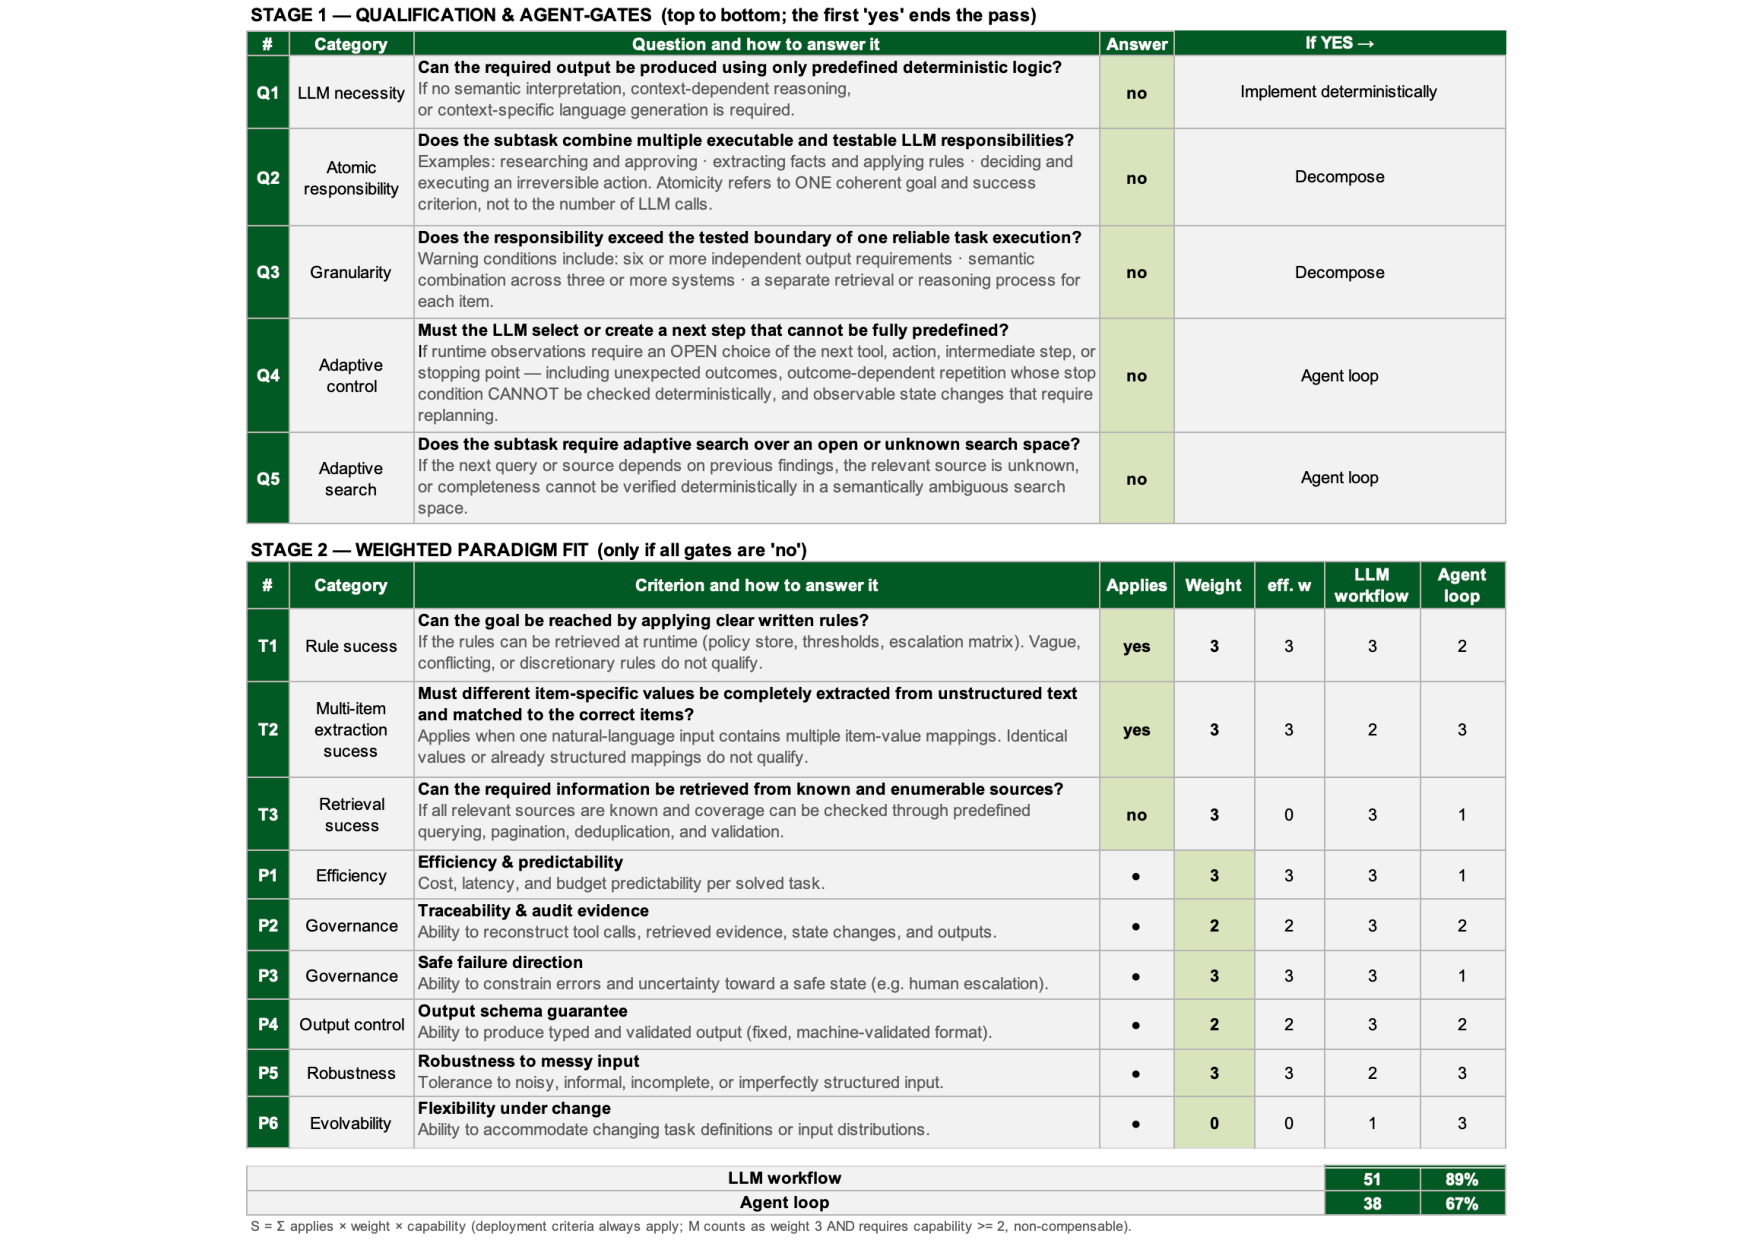
\includegraphics[width=\linewidth,trim=118 2 118 4,clip]{Figures/Initial_Framework_Excel.pdf}
\caption[The initial Decision Sheet]{The initial Decision Sheet (TADF v2.2) in Excel. The architect enters answers and weights in the green cells. \emph{agent loop} denotes the agent. The example applies T1 and T2. The totals at the bottom are the weighted sums and their share of the maximum score. The capability scores are the initial values: efficiency was later corrected, T3 and T2 were retired, and P6 is derived rather than measured (Section~\ref{subsubsec:TADF/evolution}).}
\label{fig:decision-sheet}
\end{figure}

\subsubsection{Development and Evidence}
\label{subsubsec:TADF/evolution}
\label{subsubsec:TADF/evidence}
The first difficulty was the structure of the framework. After the main experimental comparison, TADF v1 was drawn in four forms on 15 and 16 July 2026 (Appendix~\ref{app:evolution/development}). They were an ordered list of routing questions, a strict decision tree with one task dimension per level, a process view and a decision table. The tree did not hold: in the deep-dive runs of X, the suitable orchestration paradigm for rule-generated, record-specific updates depended on the model. The decision table mixed conditions that fix the route with better choices and preferences, and it computed no result. The Decision Sheet therefore became a list with two stages. The gates capture conditions that decide the route regardless of preferences, and the weighted scoring lets the architect set individual priorities. Within Stage 1, the qualification questions come first, because a task that needs no LLM or is too large should not be routed as it stands.

Q1 and Q2 came from a structured self-review of trial applications. Q1 reflects the scope of the evidence: only executions with an LLM were tested, so the framework helps only where a task needs an LLM. Tasks that predefined logic can solve therefore leave the sheet with a deterministic implementation. Q2 fixes the unit of assessment. Each pass assesses one task with one goal and one success criterion; otherwise, it would be unclear during the walkthrough whether the right unit is being assessed.

Q3 addresses tasks that are too large for one execution. At the high level of H, a draft had to meet six or seven constraints over two feedback rounds; at the high level of B, one result had to combine CRM, mail and calendar. Both orchestration paradigms stayed below 60 percent there, and no model exceeded this value (Tables~\ref{tab:app-difficulty-results} and~\ref{tab:app-high-model-results}). This may be related to the number of simultaneous requirements and systems, so Q3 recommends decomposition beyond the warning conditions drawn from these levels. The third warning condition, a separate retrieval or reasoning process for each item, rested on an F task instance with a defective outcome check; it therefore lacks a valid basis (Appendix~\ref{app:evolution/evidence}). Record volume alone did not qualify: in L, more records raised token cost without lowering success (Table~\ref{tab:deepdive-results}).

Q4 selects the agent when the next step depends on what happens during execution. In the three F task instances whose later actions depended on earlier outcomes, the agent solved 13 of 15 executions and the LLM workflow none (Table~\ref{tab:app-main-contrasts}). The deep-dive runs showed the same pattern for repetition until an outcome, for rules applied to outcomes and for observable state changes (P-b, X-1 and M-1 in Table~\ref{tab:deepdive-results}). The LLM workflow plans its actions before it sees their outcomes, so these tasks require an agent. S showed, however, that a state-machine LLM workflow handles outcome branches that are known in advance, so Q4 asks only for an open choice of the next step. Silent state changes defeated both orchestration paradigms (M-2) and therefore became an implementation note, not a gate.

Q5 selects the agent for adaptive search. At the high level of A, a search result determines the next query. There, the agent solved 23 of 25 executions and the LLM workflow 14, and the agent was more successful with every model (Tables~\ref{tab:app-difficulty-results} and~\ref{tab:app-high-model-results}). When the source of a needed fact was unknown (P-c), the agent solved 24 of 25 executions and the LLM workflow 12 (Table~\ref{tab:deepdive-results}).

Stage 2 scores the remaining differences. A task-fit criterion enters only if the two orchestration paradigms fall into different success bands, which are set at 90 and 50 percent. The band then sets the capability score. Table~\ref{tab:initial-evidence} in Appendix~\ref{app:evolution/evidence} gives the basis of each score. Rule success (T1) favors the LLM workflow: with code applying D's written rules, it returned the reference decision in all 75 executions and the agent in 60 (Table~\ref{tab:grid-results}). Extraction success (T2) and retrieval success (T3) rested on the confirmation test and on a development result of B. Among the deployment indicators, the LLM workflow scores higher on efficiency, because the agent used more tokens per success in six task archetypes (Table~\ref{tab:app-token-results}). It also scores higher on safe failure, because twelve of the agent's fifteen incorrect decisions in D were less restrictive than required. Traceability and schema guarantee favor the LLM workflow, whose traces and typed outputs follow from its construction. The agent scores higher on robustness to messy input, based on B's perturbation variants (Table~\ref{tab:app-robustness-results}), and on evolvability, which was derived rather than measured. At the bottom of the sheet, one total per orchestration paradigm summarizes this scoring for the priorities of the architect.

Version 2.2 fixed these rules. Before the freeze, mechanical checks confirmed that the rules return a result for every combination of gate and applicability answers. They also reproduced the expected routes of 49 reference and development cases (Appendix~\ref{app:evolution/verification}). The bands, weights and warning conditions remain design choices, not estimated probabilities. Later audits corrected three elements. The declared efficiency median of 3.6 did not reproduce; the eight task archetypes give 2.21 (Table~\ref{tab:app-token-results}). T3's development result was not reproduced by the main experimental comparison. The task instance behind T2 gives all nine records the same value, so the confirmation test did not measure item-specific values. T3 and T2 were therefore retired before submission (Section~\ref{subsubsec:TADF/artifact-correction}).

\subsubsection{Retrospective Routing Comparison}
\label{subsubsec:TADF/functionality}
A retrospective comparison on the development data gives a first indication of routing value (O5). It applies the archived group-level routes of the Decision Sheet to 17 result groups from the main experimental comparison and the deep-dive runs, with 710 execution slots per strategy (Figure~\ref{fig:routing-value}). The references are always agent, always LLM workflow, random selection and a group-wise oracle and its opposite, which choose the more and the less successful orchestration paradigm per group. The Decision Sheet matched the success of always agent, 82.5 percent, with 6,832 instead of 12,851 recorded tokens per successful execution. Compared with always agent, its routes lost 21 successful executions in B, C, L, S-1 and S-2 and gained 21 in D and E. The oracle was 3.0 percentage points more successful.

\begin{figure}[htbp]
\centering
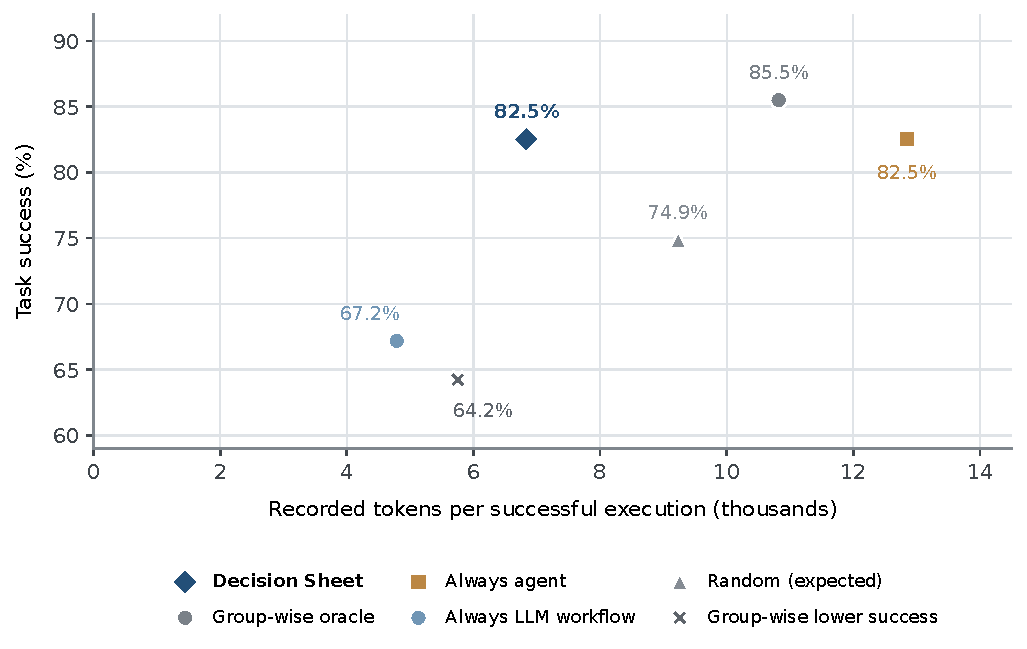
\includegraphics[width=0.8\linewidth]{Figures/fig_routing_value.pdf}
\caption[Retrospective Routing Comparison.]{Retrospective Routing Comparison. Task success and recorded tokens per successful execution of six routing strategies on the development data. Each strategy covers 710 execution slots in 17 result groups. The LLM workflow side includes the state-machine LLM workflow on S-1 and S-2. Costs use the available token observations.}
\label{fig:routing-value}
\end{figure}

The comparison is retrospective. Its groups and routes come from the data that shaped the rules, and the routes apply to groups rather than to single tasks. Repeated executions of a task instance are also not independent. It indicates routing value on the development data only; the evaluation in Section~\ref{subsec:TADF/evaluation} examines the framework beyond them. Appendix~\ref{app:evolution/portfolio} specifies the groups and the calculation.
\FloatBarrier

\subsection{Evaluation}
\label{subsec:TADF/evaluation}
Two evaluation episodes assessed TADF against the design objectives in Section~\ref{subsec:TADF/objectives}. In Episode~1, practitioners described their decision practice and judged the initial Decision Sheet. In Episode~2, the revised framework gave recommendations for WorkBench, and routed execution was compared with using one orchestration paradigm for all tasks. Both episodes led to revisions, following the iterative evaluation activity of DSRM \parencite{peffersDesignScienceResearch2007}. Each episode therefore reports the evaluated version, the findings and the resulting changes.

\subsubsection{Episode 1: Practitioner Interviews}
\label{subsubsec:TADF/episode1}
Episode~1 addressed SQ3 from the perspective of practitioners (Section~\ref{subsec:intro/scope}). It examined whether the choice between the two orchestration paradigms arises in practice, how it is made today, whether the Decision Sheet is understandable and what should change. The sample therefore aimed at people who face this choice in their own work. The inclusion criterion was hands-on experience in building agentic systems or LLM workflow automations. Twelve participants were recruited through LinkedIn, Fiverr and personal contacts. Seven build or advise on AI automations for clients (P02--P07, P09). The others are two engineers, a marketing entrepreneur, the founder of an AI-adoption consultancy and a specialized student (Appendix~\ref{app:eval1/participants}). Together, they cover settings from small businesses to legal, financial and industrial organizations, as well as workflow platforms and agent tools. They thus make the decision that TADF supports, even where their role is not called software architect.

Between 5 and 17 August 2026, ten participants took part in recorded online sessions with screen sharing, nine in German and one in English. P02 and P03 received the Decision Sheet and the questions and answered in writing. A semi-structured guide gave all interviews a common structure: main questions with optional follow-up questions that allowed open answers \parencite{myersQualitativeInterviewResearch2007}. Its five blocks covered the participant's role, a short presentation of the research, the current decision practice, a walkthrough of the Decision Sheet and an open closing question (Appendix~\ref{app:eval1/guide}). P02 and P03 also applied the sheet to a task from their practice. Each interview or written response was anonymized and condensed into a structured record that follows the blocks of the guide. The records keep the participants' statements apart from the interviewer's input and from analytic notes. They were compared in four categories taken from the guide: the relevance of the choice, the current decision practice, the understanding and logic of the Decision Sheet, and improvements. The participant IDs refer to the records in the repository (Appendix~\ref{app:repository}).

The interviews confirmed that the choice arises in practice. All twelve participants described it from their own projects. P02 reported that it comes up increasingly in client discussions. P06 reported clients who ask for an agent because the term is popular, although a simpler solution would suffice. P12 considered the task level relevant because larger automations contain parts with different requirements. P11 also saw the problem as relevant but questioned whether LLM workflows and agents can always be separated cleanly.

In current practice, the choice rests on experience. Ten participants made it by experience, intuition, client preference or platform defaults, without a formal method (P01, P02, P04--P10, P12). Their rules of thumb were similar. A predictable sequence with known outputs led to an LLM workflow. A next step, source or output that could not be listed in advance led to an agent (P02, P03, P06, P07). Four participants kept agents to bounded parts of a workflow (P02--P04, P09), and P10 turned validated agent solutions into reusable workflows. Irreversible actions required deterministic control or human approval (P02, P03, P12). Data protection or approved platforms could rule out a design (P07, P11), and cost was a main criterion for P08, P09 and P12. No record describes a procedure that combines task characteristics, comparative evidence, constraints and priorities. This supports the research gap in Section~\ref{subsec:intro/problem}: the choice recurs in practice, but it rests on rules of thumb.

The Decision Sheet was largely understood. Eight participants found the two stages, gates before a weighted comparison, understandable or consistent with their experience (P01--P04, P06, P08--P10). P01 especially supported the first question, which routes a task to deterministic code if no LLM is needed, and P07 considered both agent gates plausible. P02 and P03 applied the sheet to lead-handling tasks. In both cases, it favored an LLM workflow, which matched their production design or expectation. For P03, the LLM workflow scored 47 and the agent 32 of 51 points, and the mandatory safe-failure marking excluded the agent. P02's production system still passed unclear messages, about one fifth, to a bounded agent step. Unclear points concerned the unit of assessment in Q2 (P02, P03), the basis of the warning conditions in Q3 (P03, P07) and the meaning of Q4 (P02, P03, P11). P01 questioned the schema advantage of the LLM workflow, and P07 found labels and totals hard to read and warned against double counting. The agreement came after the interviewer had explained the sheet, so it shows perceived plausibility rather than independent validation.

The suggested improvements concerned the form of the framework, its scope and its rules. The redesign to TADF v3 adopted the following changes. Table~\ref{tab:eval1-improvements} lists all suggestions, including those not adopted, with the reasons. First, the spreadsheet did not fit how the participants work. Half of them already plan or build automations with LLM assistants or coding agents (P04--P07, P11, P12). Several did not want to fill in a separate spreadsheet for every decision (P04, P08, P11, P12), and the sheet took time or was dense (P01, P05). Participants asked for guided use (P04, P07) or supported an LLM assistant or skill that they could use directly in their work (P05, P06, P08, P11, P12). TADF v3 is therefore delivered as a skill for an LLM assistant. This form also aims at the objective of bounded effort (O7).

Second, metrics’s like task success and token cost alone did not decide the choice. Participants named the environment, such as client requirements, approved platforms, existing tools, data protection, hosting and the people who maintain the solution (P03--P07, P09, P11). They also named the goal of the system. P10 asked whether it should improve through feedback or run a stable procedure, and P11 whether it should assist experts or automate fully. The lifecycle of the system mattered as well, from one-off use to recurring operation and from a prototype to production (P04, P09, P12). The redesign therefore captures the objective and lifecycle of the system before the tasks are assessed. Each recommendation for an LLM workflow or agent also includes checks of the environment.

Third, the distinction and its evidence had to be explained. Several participants asked what exactly separates an LLM workflow from an agent, or used the terms in other ways (P01, P05, P11). Explanations with examples were seen as helpful (P03, P06, P07), and P07 wanted to see the evidence behind a recommendation and the answers that decided it. TADF v3 therefore contains definitions of both orchestration paradigms with measured examples, which the architect can ask about. It also names the evidence behind each recommendation and documents the answers in a decision record (P04, P06, P07, P11, P12). Fourth, participants needed guidance after the route: how to build the chosen design and which safeguards it needs (P09--P11). They named loop limits, logging, output validation and an independent verifier (P01, P02, P08, P10, P12). Each recommendation for an LLM workflow or agent now includes this design knowledge.

Fifth, hard limits and preferences were separated. Irreversible actions needed human approval (P02, P03, P10, P12), and a weighted score should not offset this requirement (P02, P03). A consequential action without a tested rollback therefore requires human approval on every route. Cost and latency are treated separately because their importance differs (P07, P09). The fixed capability scores are kept apart from the architect's weights to avoid double counting (P07). Build effort stays outside the scoring, because coding agents have reduced the effort of building workflows (P04, P07). Finally, the gates were renamed G1--G5, and their questions were sharpened where participants had found them unclear (P02, P03, P06, P07, P11). The framework also states that only the ReAct agent was measured and that the choice of model can change the result (P01, P09, P12).

\subsubsection{Episode 2: WorkBench Evaluation}
\label{subsubsec:TADF/episode2}
\label{subsubsec:TADF/pilots}
Episode~2 addressed the second part of SQ3 (Section~\ref{subsec:intro/scope}). It examined whether TADF gives the same recommendations in two separate passes and whether following them leads to successful execution at low token cost. The test setting was WorkBench, a benchmark of workplace tasks in five domains, such as email and calendar \parencite{stylesWorkBenchBenchmarkDataset2024}. Its 690 task instances come from 69 templates with ten task instances each. A task instance is solved if the resulting database state matches a reference state. The evaluation used the 2026 release WorkBench Revisited, which corrected scoring, reference outcomes and prompts \parencite{stylesWorkBenchRevisitedWorkplace2026}.

WorkBench was selected because both orchestration paradigms could be built on it as this thesis defines them, with the same task instances, tools and scoring (Section~\ref{subsec:theory/workflows-agents}). Its limits were known in advance. All information lies in known databases and the set of tools is fixed, which favors predefined control. A preliminary classification had already expected an LLM workflow for all 69 templates, and open-ended search is hardly covered. WorkBench was still suitable. It tests whether the expected fit leads to more successful and cheaper execution than an agent achieves, and whether the recommendations are stable. It cannot show whether TADF selects an agent where one is needed.

The frozen TADF v3 skill was run for each of the 69 templates, because the ten task instances of a template share one structure (Appendix~\ref{app:eval2/routing}). It received only the template text and a neutral description of the environment. In its benchmark mode, G1--G3 were recorded but could not stop or split a task, so G4, G5 and the comparative assessment chose between the LLM workflow and the agent. The routing ran in two passes of six new sessions each, and the second pass reversed the order of the templates. The recommendations were saved before the evaluation runs began.

All executions used GPT-5.4-mini. The LLM workflow had the two-stage form of task archetype F (Section~\ref{subsubsec:TADF/paradigms}): model calls planned the reads and the actions, and code ran the reads and validated and executed the actions. The agent was the benchmark's own agent, used unmodified in four configurations, and its setup nearly reproduced the published result for this model (Appendices~\ref{app:eval2/freeze} and~\ref{app:eval2/results}). TADF-routed execution was compared with using one orchestration paradigm for all task instances (Always workflow, Always agent). Two strategies were computed from the executions: Random picks an orchestration paradigm per task instance with equal probability, and Oracle picks the agent only where the agent alone succeeds. Besides task success, the evaluation counted side-effect errors, that is, unsuccessful executions that changed records, and mean tokens per task instance, which were estimated from transcripts for the agent (Appendix~\ref{app:eval2/cost}).

Both passes recommended an LLM workflow for all 69 templates, and no gate fired. TADF-routed execution was therefore identical to Always workflow. The input stated no priorities, and the benchmark mode gives each deployment indicator the default weight of 2 unless the template text reveals its weight. Under such a neutral profile, the fixed capability scores favor the LLM workflow by more than the only agent-favoring task-fit criterion can offset. Only G4 or G5 can then select an agent. The agreement concerns the final recommendations, not every answer behind them.

In the first comparison (2a), LLM workflow v1 solved 287 of the 690 task instances (41.6\%). This was below all four agent configurations and matched the main experimental comparison, in which the agent was also more successful in action execution (Section~\ref{subsubsec:TADF/results}). Its best domain was email, the only one with refined prompts. On 50 development task instances from the other domain files, v1 failed 40, mainly because reads depended on earlier results, search parameters did not fit, per-item actions were missing and conditions were mishandled (Appendix~\ref{app:eval2/revision}). TADF's design knowledge already prescribed a bounded re-plan, per-item calls, a placeholder guard and conditions that fail closed, but v1 had implemented none of them. Version~v2.1 therefore added a bounded round of follow-up reads, a check in code against placeholders and unknown identifiers, and general prompt rules. It was frozen and executed on all 690 task instances with the same recommendations (comparison~2b).

With v2.1, following TADF solved 457 task instances (66.2\%), at 7,299 instead of 3,313 tokens per task instance (Figure~\ref{fig:eval2-contribution}). It exceeded the strongest agent, native tool calling with domain tools (60.9\%), by 37 task instances or 5.4 percentage points at about half its estimated token cost. This lead is uncertain, because the task instances of a template are not independent. When templates are resampled, its 95 percent interval ranges from $-1.4$ to 12.2 points (Appendix~\ref{app:eval2/limits}). The gain from v1 to v2.1, 24.6 points with an interval from 16.8 to 32.8, is clear. Random reached 63.6\%. Oracle reached 75.9\%, because the agent solved 67 task instances that v2.1 failed. Choosing in hindsight the better orchestration paradigm for each template would have reached 73.2\%. In comparison~2b, TADF-routed execution thus achieved higher success than Always agent in all four configurations, but it equaled Always workflow. The episode shows no benefit of routing itself.

\begin{figure}[htbp]
\centering
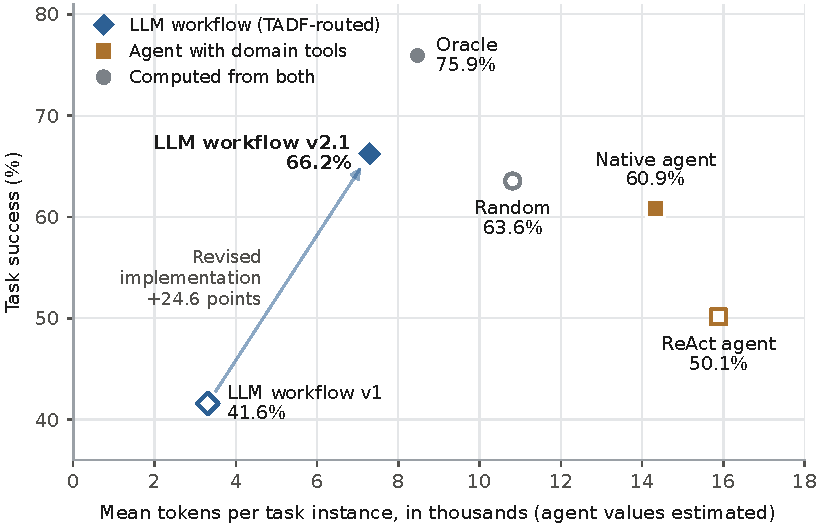
\includegraphics[width=0.94\linewidth]{Figures/fig_workbench_success_tokens.pdf}
\caption[Task success and mean tokens on WorkBench]{Task success and mean tokens per task instance on WorkBench with GPT-5.4-mini. Random and Oracle combine LLM workflow v2.1 with the native agent.}
\label{fig:eval2-contribution}
\end{figure}

Two findings matter for the thesis. First, the benefit of the same recommendations depended on whether the build followed the design knowledge. The revision changed several mechanisms at once, so the effect of single rules remains open. Second, predefined control did not prevent side-effect errors. v2.1 caused 119, fewer than v1 (148) and the native agent (134), but twice as many as the ReAct agent with domain tools (59). TADF's higher safe-failure score for the LLM workflow (P2) assumes a failure direction fixed by design, whereas v2.1 checked conditions and item counts only through its prompts.

The 60 task instances used for development remain among the 690. Without them, v2.1 reached 64.9 percent and the native agent 60.0 percent (Appendix~\ref{app:eval2/limits}). These 630 are still no independent test set, and each configuration has one result per task instance. The results therefore describe the tested implementations on this benchmark (Section~\ref{subsec:discussion/limitations}).

The episode led to three revisions of TADF (Appendix~\ref{app:eval2/framework-revision}). Because some searches return at most five records, G4 now asks whether the planned reads can show all information that the decision needs. If they cannot, G4 fires. Every LLM workflow recommendation now names a mandatory minimum: a bounded re-plan, a placeholder guard, per-item calls with a count check, conditions that fail closed and a pilot before the build is frozen. The architect confirms that the build will implement it. Otherwise, the recommendation stays conditional. Capability scores and weights stayed the same, and the new G4 question was not tested again on WorkBench. Two simulated pilot consultations then refined the dialogue, for example by confirming proposed gate answers together (Appendix~\ref{app:eval2/pilots}).
% SEC 4 - TADF
\clearpage
\section{The Task-Level Architecture Decision Framework (TADF)}
\label{sec:TADF}

Chapter 4 presents the artifact along its DSR trajectory. Section \ref{subsec:TADF/objectives}
states what the artifact must achieve (DSRM activity 2). Section \ref{subsec:TADF/design}
shows how it was built --- the design search process across development cycles, including the
controlled experiments that form its evidence base and the formative role of the two evaluation
episodes. Section \ref{subsec:TADF/artifact} describes the resulting artifact in full --- the
reader meets the frozen framework before any evidence about it is weighed. Section
\ref{subsec:TADF/evaluation} reports both evaluation episodes against the objectives of
Section \ref{subsec:TADF/objectives}. Section \ref{subsec:TADF/demonstration} demonstrates the
frozen artifact solving a complete instance of its problem class.

\subsection{Objectives of a Solution}
\label{subsec:TADF/objectives}
...

\subsection{Design and Development}
\label{subsec:TADF/design}
...

\subsection{The Artifact}
\label{subsec:TADF/artifact}
...

\subsection{Evaluation}
\label{subsec:TADF/evaluation}
...

\subsection{Demonstration}
\label{subsec:TADF/demonstration}
...

% SEC 5 - Discussion
\clearpage
\section{Discussion}
\label{sec:Discussion}

This thesis set out to support software architects in choosing between an LLM workflow and an agent for a single task in an agentic system. The results answer the research question in three parts. First, the choice matters, and practice lacks support for it. Second, a framework can support the choice in three steps. It first qualifies the task within its system context, then checks its control requirements and finally weighs the priorities of the architect, within hard limits that no weight can offset. It then attaches the conditions for building the chosen orchestration paradigm. Third, such support can work inside the architect's own LLM assistant, where the model interprets the description and code applies the fixed rules. Following \textcite{gregorPositioningPresentingDesign2013}, this chapter interprets these results against the objectives and relates them to the general problem of choosing an orchestration paradigm.

The interviews support the research gap. All twelve participants knew the choice from their own projects, and ten made it by experience, intuition, client preference or platform defaults, without a formal method (Section~\ref{subsubsec:TADF/episode1}). No participant described a procedure that combines task characteristics, comparative evidence, constraints and priorities. The experiments show that the choice has consequences. Per task archetype, the success rates of the two orchestration paradigms differed by up to 26.7 percentage points, and for single task requirements by far more. In six of eight task archetypes, the agent needed 1.8 to 7.7 times the tokens per successful execution (Section~\ref{subsubsec:TADF/results}). On WorkBench, Oracle, which chose the agent only where the agent alone succeeded, would have reached 75.9 instead of 66.2 percent. Choosing in hindsight for each template would have reached 73.2 percent (Section~\ref{subsubsec:TADF/episode2}).

Measured against the design objectives (Section~\ref{subsec:TADF/objective-results}), the strengths and gaps follow one pattern. Where the evidence came from controlled comparisons and tests, it is firmer. The decision core rests on paired executions, and code applies the rules reproducibly. Where the evidence depends on use, it is only formative. Practitioners found the logic understandable and asked for an assistant form. However, no independent architect has yet decided with TADF, and on WorkBench routing by TADF added no success beyond Always LLM workflow. The hypothesis therefore holds only in part. In the window, TADF gives traceable recommendations that are the same for the same answers, and practitioners asked for the assistant form that it now has. Its benefit on new tasks, however, remains to be shown.

Three choices of the research design proved valuable. Implementing both orchestration paradigms for the same task instances allowed a paired comparison at the task level, which earlier benchmarks did not offer. Asking practitioners before the final design turned the spreadsheet into a skill. Linking each rule to its evidence made it possible to retire rules whose evidence did not hold. The scope, in contrast, was broad: eight task archetypes, three models, deep-dive runs, two evaluation episodes and a working skill. This breadth mapped the decision but left several rules on thin evidence, and a narrower scope would have tested fewer rules more firmly. The approach still points in the right direction. The rules of thumb of practitioners matched its agent gates, and practice and research both call for explicit guidance (Section~\ref{subsec:discussion/practice}). In a young field, the broad map is also useful. It shows where the evidence is firm, where it is thin and where research can start. It also suggests how decision support for architects may look in the future: inside the tools that architects already use, and based on a versioned rulebook that grows with new evidence.

Section~\ref{subsec:discussion/findings} discusses the choice between the two orchestration paradigms (SQ1 and SQ2), Section~\ref{subsec:discussion/practice} decision support in practice (SQ3), Section~\ref{subsec:discussion/contribution} the design principles and Section~\ref{subsec:discussion/limitations} the limitations and future research.

\subsection{Choosing Between LLM Workflows and Agents}
\label{subsec:discussion/findings}

SQ1 and SQ2 asked how the two orchestration paradigms compare and which task characteristics and execution conditions are associated with their differences. Neither paradigm was better in general. That also underlines the current agentic archtecture discurse shown in \ref{sec:Background}.  The agent was more successful where the next step or the sources could not be fixed in advance, and the LLM workflow where written rules decided. In most task archetypes, the agent needed more tokens. Taken together, the results suggest that the choice is not one decision but a sequence of levels. At the level of the system context, the lifecycle frames the choice, for example one-off use or recurring production. At the level of the task boundary, G1 to G3 separate parts that need no LLM and split tasks that are too large. At the level of control, G4 and G5 decide whether only an agent can perform the task. In the weighted comparison, the priorities of the architect decide between the remaining options, within hard limits. At the level of implementation, the build form and its components decide whether the chosen orchestration paradigm succeeds. TADF follows this order, and the paradigm is only one layer of the architecture decision.

At present, the last two gates mark the clearest difference. G4 asks whether every next step can be fixed before the run, and G5 whether the sources are known in advance. Where later actions depended on earlier outcomes, the agent solved 13 of 15 executions and the LLM workflow none. Where a search result determined the next query, the agent solved 23 of 25 executions and the LLM workflow 14. Where the source of a needed fact was unknown, the result was 24 against 12 (Section~\ref{subsec:TADF/initial-artifact}). This is the strength of the agent: it chooses the next step from what it observes. Control also depends on what can be observed. Neither paradigm succeeded when a state changed silently, and the agent recovered in only 16 of 25 executions when the procedure required a new check (Section~\ref{subsubsec:TADF/results}). On WorkBench, capped searches hid records, which added the question about the planned reads to G4 (Section~\ref{subsubsec:TADF/episode2}). Practitioners used the same distinction in their rules of thumb (P02, P03, P06, P07). It sharpens practitioner guidance that reserves agents for tasks that need flexibility or where rule-based approaches fall short \parencite{schluntzBuildingEffectiveAI2024,openaiPracticalGuideAgents2026}. The number of actions alone, in contrast, did not decide. When a read set the number of actions, both paradigms solved all 25 executions, and the LLM workflow needed roughly a third of the agent's mean token cost. Where outcome branches were known in advance, a state-machine LLM workflow solved 19 and 14 of 25 executions, against 24 and 15 for the agent (Section~\ref{subsubsec:TADF/results}).

Outside these two gates, the choice is a trade-off, and here the deployment indicators mostly favor the LLM workflow. It applied written rules more reliably and returned the reference decision in all 75 executions, against 60 for the agent. It also needed fewer tokens per successful execution in six of eight task archetypes. This supports judging success together with cost \parencite{kapoorAIAgentsThat2024}. In retrieval and planning, the agent was more successful, but these differences remain uncertain. Under equal weights, the fixed capability scores favor the LLM workflow, so that only G4 or G5 can select an agent (Appendix~\ref{app:artifact/scoring}). The agent leads only on robustness to messy input and evolvability, and evolvability was derived rather than measured. On the comparative path, the priorities of the architect thus decide. TADF recommends the LLM workflow when cost, safe failure and schema guarantee weigh highly. It recommends the agent only when robustness to messy input and evolvability weigh well above them. The LLM workflow has clear weaknesses, too. Predefined control does not ensure correct execution. On WorkBench, the revised LLM workflow was more successful than the ReAct agent with domain tools but caused 119 side-effect errors against 59 (Section~\ref{subsubsec:TADF/episode2}). Its success also depends on the build, as two implementations of the LLM workflow reached 41.6 and 66.2 percent.

These findings are consistent with what practice reports at the system level. Cost and reliability limit the use of agentic systems (Section~\ref{subsec:intro/motivation}), and 68 percent of deployed agents run at most ten steps before a person intervenes \parencite{panMeasuringAgentsProduction2025}. Gartner expects that over 40 percent of agentic AI projects will be canceled by the end of 2027. It names rising costs, unclear business value and inadequate risk controls, and it notes that many use cases presented as agentic do not need an agentic implementation \parencite{gartnerGartnerPredictsOver2025}. P06 reported clients who asked for an agent because the term was popular, although a simpler solution would have sufficed. Model providers likewise advise starting with the simplest solution, because agents trade latency and cost for task performance \parencite{schluntzBuildingEffectiveAI2024,openaiPracticalGuideAgents2026}. Research on workflow optimization recommends starting from a constrained static structure and reserving changes during execution for settings in which execution reveals information that a plan cannot anticipate \parencite{yueStaticTemplatesDynamic2026}. More agents do not help by default either. Under a shared protocol, only one of six multi-agent systems exceeded a single-agent baseline, and its small lead was within the reported uncertainty \parencite{fuDoMoreAgentsHelp2026}. For workplace automation in production, the evidence therefore suggests a default for current models: an LLM workflow, unless G4 or G5 applies. Where these gates apply, practice tends to bound the agent or to keep a person in the loop. Practitioners kept agents to bounded parts of a workflow (P02--P04, P09), and P10 turned validated agent solutions into workflows. Research follows the same path: \textcite{abuzakukOptimizingAgenticWorkflows2026} compile recurring tool-call sequences of an agent into deterministic composite tools. In practice, the agent is thus less a rival of the LLM workflow than a bounded component for the parts that cannot be fixed in advance.

Before production, the agent has a clear strength. In the seven task archetypes with tools, the same prebuilt ReAct agent reached 70.7 to 100 percent task success. Each LLM workflow, in contrast, had to be built as a graph for its individual task archetype (Sections~\ref{subsubsec:TADF/paradigms} and~\ref{subsubsec:TADF/results}). The agent needs no procedure designed for the task. For non-recurring tasks, proofs of concept and daily work in which the goal is not yet clear, this saves design effort that an LLM workflow repays only through repeated use. Practitioners distinguished one-off from recurring use and prototypes from production (P04, P09, P12), and P10 turned validated agent solutions into workflows. The agent can thus explore the path, and the LLM workflow can fix it once the task recurs. The build effort itself was not measured (Section~\ref{subsec:discussion/limitations}).

This boundary is not fixed. With GPT-5.2 instead of GPT-5.4-nano, the agent's gap to the LLM workflow in compliance narrowed from 23.3 to 6.7 percentage points (Section~\ref{subsubsec:TADF/results}). On a revised WorkBench, the best agent reached 97.7 percent, although that study also changed the execution interface and corrected benchmark defects \parencite{stylesWorkBenchRevisitedWorkplace2026}. In simulated dialogues, a model that executed a procedure from its prompt reached higher judged task success than a code-controlled graph, but at higher token cost \parencite{dennisInContextPromptingObsoletes2026}. The gains of multi-agent designs also vary with task structure and model capability \parencite{kimScienceScalingAgent2025}. If stronger models close the success gap, cost, traceability and safeguards would weigh more. Falling prices could weaken the cost argument, but token use for complex tasks has so far grown faster than the price per token has fallen \parencite{tinkoffStateAI2026}. The default above is therefore a statement about current models, not a lasting rule.

The breadth of the scope also limits how far these conclusions reach. Each task archetype had 15 task instances, and the deep-dive runs examined only action execution. Part of each difference may stem from the implementations rather than from the paradigm, because the paired systems also differed slightly in prompts and deterministic components (Appendix~\ref{app:protocol/implementation}). G4, G5 and the cost difference rest on clear and repeated differences. Other rules rest on single comparisons, and two task-fit criteria were retired when their evidence did not hold (Section~\ref{subsubsec:TADF/artifact-correction}). The findings therefore support a direction rather than a settled rule set: predefined control first, and model control where the next step or the sources cannot be fixed in advance.

\subsection{Architecture Decision Support in Practice}
\label{subsec:discussion/practice}

SQ3 asked how relevant the distinction is in practice and how far TADF supports architects. The distinction is relevant, and both the interviews and the literature call for support of this kind. All participants knew the choice from their projects, and P01, P02 and P06 saw value in making it explicit. Half of the participants already plan or build automations with LLM assistants or coding agents (P04--P07, P11, P12). Five supported an LLM assistant or skill that they could use directly in their work (P05, P06, P08, P11, P12). Engineering teams often lack clear guidance on how to put agentic systems into operation \parencite{bandaraPracticalGuideAgentic2026}. A proposal for AI-based architecture decision support likewise combines explained recommendations with decision records, but reports only a preliminary evaluation \parencite{arifAIDrivenDecisionSupport2025}. TADF shows one way to meet this demand. The consultation starts from the architect's own description, the assistant proposes answers with reasons, code applies the fixed rules and the architect confirms. This allocation follows the assisting archetype of agentic information systems, in which the human keeps the main responsibility \parencite{holldackAgenticInformationSystems2026}. As LLM assistants become common tools of architects, such support may well spread. Its effect on the decisions of independent architects, however, is not yet tested.

The interviews also explain why the framework grew large. Performance alone did not settle the choice. Approved platforms and data protection could rule out a design (P07, P11), and data readiness could constrain it (P12). Approval before irreversible actions was a hard limit, not a preference (P02, P03, P10, P12). Such safeguards are not always built: among 6,003 public n8n templates, only 167 contained a human-mediated path before external actions \parencite{tangCharacterizingLargeLanguage2026}. Most of these factors entered TADF. The system context frames the consultation, mandatory markings and the approval rule act as hard limits, and environment checks follow each route. Data readiness remains for the architect to check. More coverage means more effort, a tension known from architecture decision methods \parencite{falessiDecisionmakingTechniquesSoftware2011} that the window eases. Even so, the current evidence does not allow a certain decision for every task. Further research will likely add factors, such as multi-agent coordination, other model families or security requirements. Design science research with generative AI faces a rapid erosion of prescriptive knowledge \parencite{zurheidenDesignScienceResearch2026}. TADF is therefore best understood as a living framework. In medicine, living guidelines update a single recommendation as soon as new evidence becomes available, so that the unit of update is the recommendation, not the whole guideline \parencite{aklLivingSystematicReviews2017}. TADF was developed in this way. Each rule names its evidence, each evaluated state was frozen, and the development log records every change, including the retirement of two task-fit criteria. Continuing this practice beyond the thesis would keep the framework current.

The task level is central to this support, but it is hard to delimit in practice. A task is the unit that receives a route, yet the same work can form one task or several. In the text and the window consultation of the CrewAI email scenario, draft writing was split into two tasks once and kept as one task once. The difference came from the architect's gate answers (Appendices~\ref{app:transcripts/audit} and~\ref{app:transcripts/window}). Participants found the unit of assessment unclear (P02, P03), and P11 doubted that LLM workflows and agents can always be separated cleanly for one task. TADF limits the problem with explicit split rules and a limit of two split-or-simplify operations per task lineage, but it cannot define the tasks for the architect. Making task boundaries tangible, for example through worked examples or links to existing process models, is a practical need for future versions.

Much recent research addresses the choice at run time. Routers select a model, a reasoning strategy or a single-agent or multi-agent configuration for each incoming request \parencite{gaoSingleagentMultiagentSystems2025,suDifficultyAwareAgenticOrchestration2025,zhouSelectthenSolveParadigmRouting2026}. Search methods generate and test agent designs automatically \parencite{huAutomatedDesignAgentic2024}. These approaches react to each request or need executions of candidate designs. TADF acts earlier, when the architect decides what to build and must justify the choice against constraints and priorities. The two forms can complement each other. Design-time advice could fix the acceptable options, and a validated router could choose among them at run time. Decision support for architects may thus develop into a living, assistant-based consultation that combines evidence-based rules at design time with selection at run time and learns from the decision records of deployed systems. This combination has not been evaluated but is seen as a good way for future decisions support systems.

The demonstration also showed where the assistant must not decide alone. In the walkthrough of 27 August 2026, the assistant changed score contributions and omitted a required step despite fixed documents (Appendix~\ref{app:transcripts/audit}). The final skill therefore lets code apply the rules. Tests confirmed that this code reproduces every tested route, and in test consultations the window cut the consultation time by about 75 to 80 percent (Section~\ref{subsubsec:TADF/artifact-correction}). TADF thus applies the main finding of this thesis to itself: the model interprets, and predefined code controls the procedure. The tests cover the rule code, not the interpretation of descriptions, and where a host cannot show interactive pages, the text mode again leaves rule application to the model. Human confirmation remains a weak point. Professionals may accept or reject AI advice without examining its basis \parencite{jussupowAugmentingMedicalDiagnosis2021,lebovitzEngageNotEngage2022}, so a confirmed proposal is not necessarily a checked one.

For practice, three implications follow. Software architects can treat the LLM workflow as the default for current models, use an agent where G4 or G5 applies and implement the mandatory minimum. Clients and managers can ask whether a task needs an agent before they pay for one (P06). Builders of assistants and automation platforms can keep rule application in code and make approval paths easy to add.

\subsection{Design Principles}
\label{subsec:discussion/contribution}

Together with the comparative evidence, the decision method of TADF and four design principles form the knowledge contribution of the thesis. The catalogue of 18 agent design patterns of \textcite{liuAgentDesignPattern2025} links design choices to qualitative trade-offs. TADF addresses a narrower choice but connects it to paired executions. In the terms of \textcite{gregorPositioningPresentingDesign2013}, the work is an improvement: it offers an explicit, evidence-linked procedure for a known decision that practice addresses with heuristics. The skill is a situated instantiation at Level~1. The decision method and the principles are nascent design knowledge at Level~2. The method comprises gates before scoring, fixed capability scores and design knowledge with a mandatory minimum. A well-developed design theory is not claimed. The principles were derived from the design and the formative evaluation of TADF, which instantiates them. Whether other designers find them understandable and useful, and whether instances built from them improve decisions, remains to be tested, ideally in contrasting settings \parencite{australiannationaluniversityaustraliaResearchPerspectivesAnatomy2020,seidelDesignPrinciplesSensemaking2018}.

 The four principles describe decision support for the choice between LLM workflows and agents, of which TADF is one instance. They follow the schema of \textcite{australiannationaluniversityaustraliaResearchPerspectivesAnatomy2020}: for implementers to achieve or allow an aim for users in a context, employ mechanisms, involving enactors, because of a rationale. The implementers are researchers and developers who build such decision support. The users are software architects who decide before implementation, and the enactors are the architect, an LLM assistant and code. All four principles share one context, which also sets their boundary conditions: the task-level choice in agentic workplace automation with current LLMs.

DP1 to DP3 address, in this order, the three components of a DSS (Section~\ref{subsec:theory/decision-support}): the decision model, the data (here the evidence behind the rules) and the dialogue with the user. DP4 adds the division of work between the assistant, code and the architect, a question that arises when an LLM conducts the dialogue. The principles take up the design objectives of Section~\ref{subsec:TADF/objectives} (DP1: O1, O2, O7; DP2: O3, O6, O8; DP3: O7; DP4: O4), but not O5, because better decisions on new tasks remain unestablished. DP1 to DP3 use allow, because the architect and the assistant act in them, and DP4 uses achieve, because code turns the same input into the same output \parencite{australiannationaluniversityaustraliaResearchPerspectivesAnatomy2020}. Each principle gives its statement, mechanism, rationale, instantiation in TADF and limits.

\paragraph{DP1: Decide from coarse to fine.}
\emph{To allow software architects to reach a well-founded choice of the orchestration paradigm with bounded effort, decision support should resolve the choice in levels, from coarse cut-offs to fine weighting, within hard limits that no weight can offset.} The principle uses the first four levels of Section~\ref{subsec:discussion/findings} in their order: the system context with its lifecycle, the task boundary, the control requirements and the priorities. Coarse levels can end clear cases early, and finer levels refine the rest. Hard requirements, such as approval before consequential actions, hold on every route. In architecture decisions, constraints and minimum levels decide which alternatives are feasible before preferences rank them \parencite{falessiDecisionmakingTechniquesSoftware2011,amellerLinkingQualityAttributes2012}, and task-technology fit points to the control that a task needs \parencite{goodhueTaskTechnologyFitIndividual1995}. Empirically, the lifecycle mattered to practitioners (P04, P09, P12), G4 and G5 separated the paradigms most clearly, and the priorities decided the remaining cases (Section~\ref{subsec:discussion/findings}). TADF instantiates the task boundary, the control requirements and the priorities as G1 to G5 and a weighted comparison with mandatory markings. Its system context, however, shapes only the design knowledge and does not yet end a decision early. The order of the levels and its effect on effort were not tested against alternatives.

\paragraph{DP2: State the implementation behind every recommendation.}
\emph{To allow software architects to judge whether a recommendation fits their build, decision support should state the implementation, the model and the conditions for which its evidence holds, and attach what a build needs to match them.} DP2 covers the last level of Section~\ref{subsec:discussion/findings}, the implementation, because the labels LLM workflow and agent are not enough. Evidence holds only for the tasks, technologies and conditions it covers (Section~\ref{subsec:theory/decision-support}). On WorkBench, implementations under one label differed widely: four configurations of the benchmark's agent reached 43.0 to 60.9 percent, and two implementations of the LLM workflow 41.6 and 66.2 percent (Appendix~\ref{app:eval2/results}). Several results also changed with the model (Section~\ref{subsubsec:TADF/results}). Stating these conditions lets researchers compare and accumulate results, and it shows when a recommendation must be revised, as when TADF retired two task-fit criteria. TADF states that its evidence on agents comes from a ReAct agent and that the model can change the result. It names a leading build form with its build rules, and it asks for a commitment to the mandatory minimum. The effect of single components was not isolated, and environment checks follow the route instead of being asked beforehand.

\paragraph{DP3: Provide the consultation where architects already work.}
\emph{To allow software architects to use decision support in their daily work, decision support should provide its consultation within the environments they already use.} Currently, these include LLM assistants and coding agents, which can load decision support as a skill, a reusable package of instructions, reference documents and code. Users of decision support can often decide whether to use it, so ease of use matters, and explanations that require less effort are used more \parencite{spragueFrameworkDevelopmentDecision1980,gregorExplanationsIntelligentSystems1999}. Half of the participants already plan or build automations with LLM assistants or coding agents, and four did not want to fill in a separate spreadsheet for every decision (Section~\ref{subsubsec:TADF/episode1}). Skills are spreading as a format for these assistants: one marketplace listed 40,285 public skills, with a strong concentration on software engineering workflows \parencite{lingAgentSkillsDataDriven2026}. TADF instantiates the principle as a skill whose window cut the consultation time by about 75 to 80 percent in test consultations comared to naormal conversation questions (Section~\ref{subsubsec:TADF/artifact-correction}). Use by independent architects was not tested. The principle leaves the form open, and a skill requires assistants that can load it.

\paragraph{DP4: Let code apply the rules.}
\emph{To achieve recommendations for software architects that follow the rulebook and are the same for the same answers, decision support should let code apply its rules, while the assistant proposes the answers and the architect confirms them.} From documents alone, the assistant deviated from the rules in the walkthrough (Section~\ref{subsec:discussion/practice}), an instance of the fragile internal consistency of generative AI artifacts \parencite{zurheidenDesignScienceResearch2026}. Code, in contrast, applies the rules the same way every time. The experiments point the same way: written rules were applied more reliably under predefined control (Section~\ref{subsec:discussion/findings}). In TADF, the window applies the rules in code. Tests showed that it reproduces every route of the text consultations, agrees with an independent implementation of the rule text on 20,000 random answer sets and rules out the deviations of the walkthrough (Appendix~\ref{app:artifact/files}). In the window consultations, the architect kept 58 of the 64 proposed answers and changed six (Appendix~\ref{app:transcripts/window}). The limits of Section~\ref{subsec:discussion/practice} remain: the tests do not cover the interpretation of descriptions, the text mode leaves rule application to the assistant, and a confirmed proposal is not necessarily a checked one.

\subsection{Limitations and Future Research}
\label{subsec:discussion/limitations}
\label{subsec:discussion/future}
The results are limited in six areas. Two concern all results: the pace of the field and the independence of the research. Four concern single parts: the taxonomy, the task as the unit of decision, the size of the evaluation, and the benchmark mode together with the scoring model and the build effort. 

Two limitations apply to all results. First, the field moves fast. New models appear several times a year, and several results already depended on the model (Section~\ref{subsec:discussion/findings}). Every capability score and rule is therefore a snapshot. A fixed regression set that is rerun when models or implementations change would keep the evidence current. Second, development and evaluation were not fully independent. Tasks, implementations and rules were refined together, and one analyst built the taxonomy and condensed the interviews. The builder of TADF also took the architect role in the pilots, the demonstration and iterations. The results therefore show what the instrument can do in the hands of its builder. Independent replication is the most direct remedy.

The taxonomy covers a selected part of workplace automation. Thirteen of 48 benchmark sources were included, and the 120 task instances were constructed for this thesis (Appendix~\ref{app:taxonomy}). The deep-dive runs concern only action execution, the agent of the experiments was a ReAct loop, and the main experimental comparison used three OpenAI models. The pattern across task archetypes is therefore descriptive, not a ranking of the paradigms. Future research should code task requirements independently and add task families with open sources and long chains of outcome-dependent steps. It should also include other model families, agent designs and multi-agent coordination.

The task as the unit of decision is the most fragile construct. It makes the choice manageable, but its boundary depends on judgment, and a different boundary can change the route without any change in the work (Section~\ref{subsec:discussion/practice}). Research should study how architects delimit tasks in real systems and test whether independent architects draw the same boundaries for the same description. From such studies, criteria or reference examples for task boundaries could be derived.

The evaluation was small. Ten interviews and two written responses from a non-probability sample gave formative feedback. In the interviews, the interviewer explained the Decision Sheet before participants assessed it. Each task archetype had 15 task instances, and GPT-5.2 ran each task instance once per paradigm. One outcome check in task archetype F rejected even complete executions, although excluding it does not change the direction or the test result for F (Appendix~\ref{app:results/contrasts}). On WorkBench, one model was used, the development tasks remained in the test set, and the LLM workflow was revised after observed failures (Appendix~\ref{app:eval2/limits}). The lead of the LLM workflow over the strongest agent also remains uncertain, because the task instances of a template are not independent. An LLM judge with limited calibration and incomplete token records further limit some comparisons (Appendices~\ref{app:protocol/judges} and~\ref{app:protocol/metrics}). Future evaluations should freeze the framework and the implementations before testing, use independently selected task families as a hold-out set and repeat executions across model families.

Most importantly, no independent architect has yet used TADF to make a decision. In Episode~2, the benchmark mode bypassed the exits of G1 to G3 and used default priorities, under which only G4 or G5 could select an agent. WorkBench also favors predefined control, because all information lies in known databases, and it had informed the construction of earlier task instances. The episode therefore tested a narrow part of the procedure. It showed no routing value beyond Always LLM workflow and could not show whether TADF selects an agent where one is needed. TADF is designed for software architects, who bring constraints and priorities that a benchmark does not contain. The next study should therefore let independent architects decide comparable design cases with TADF, with their usual practice and with a simple decision aid. Assessors who do not know the decision method should judge the decisions and the success and cost of the resulting prototypes against criteria fixed in advance. Consultation time, the detection of misleading proposals and the stability across host models and paraphrased descriptions should be measured as well. In terms of FEDS, this would move the evaluation from formative and artificial settings to summative and naturalistic ones \parencite{venableFEDSFrameworkEvaluation2016}. Finally, the scoring model is a design proposal. Capability bands, fixed task-fit weights and aggregation rules were chosen for the instrument, not estimated, and their sensitivity to other thresholds was not tested (Appendix~\ref{app:artifact/scoring}). Sensitivity analyses would show how robust the recommendations are. The build effort of the two paradigms was not measured either. TADF keeps it out of the scoring and uses the system context, such as one-off or recurring use, only to scale the build effort in its design knowledge. Because coding agents now help to build LLM workflows (P04, P07), the gap in build effort is hard to assess and may shrink. Token costs also exclude development and maintenance. Future research should measure the build and maintenance effort of both paradigms, with and without coding assistants.

These limits do not remove the value of the work. In a young field, the thesis provides paired evidence at the task level, a working instrument and design principles that future research can test, extend and revise.
% SEC 6 - Conclusion
\clearpage
\section{Conclusion}
\label{sec:Conclusion}
\label{sec:conclusion}

Agentic systems take over multi-step work in organizations, but cost and reliability still limit their use. For every task of such a system, a software architect must decide whether predefined code or the model controls the progression of the task. Practice has made this choice by experience and rules of thumb, and no reviewed approach combined task characteristics, comparative evidence, constraints and priorities to support it. This thesis therefore asked how a task-level architecture decision framework can support this choice. Following design science research, it built TADF on paired implementations of both orchestration paradigms and revised it through practitioner interviews, a benchmark evaluation and a demonstration.

The paired comparison shows that neither orchestration paradigm is better in general. The agent pays off where the next step or the sources cannot be fixed before the run. Where later actions depended on earlier outcomes, it solved 13 of 15 executions and the LLM workflow none. Where written rules decided, the LLM workflow was more reliable, and in six of eight task archetypes the agent needed 1.8 to 7.7 times the tokens per successful execution. The choice is therefore a sequence of levels rather than one decision. For current models and production systems, the evidence suggests the LLM workflow as the default and the agent as a bounded component for the parts that cannot be fixed in advance.

The answer to the research question is a framework that follows these levels. TADF qualifies a task within its system context, checks whether its control requirements call for an agent and then weighs the priorities of the architect, within hard limits that no weight can offset. Each recommendation names its evidence and adds the design knowledge for building it, including a mandatory minimum for every LLM workflow. In its final form for this thesis, TADF is a skill for an LLM. The model interprets the description, code applies the fixed rules and the architect confirms. The evaluation supports this design in part. Several practitioners favored such support inside their LLM assistants and the current discurse also point ito that direction. Because code applies the rules, the same answers lead to the same recommendation. On WorkBench, however, routing by TADF only equaled Always LLM workflow, and no independent architect has yet decided with TADF. The hypothesis of consistent and practically useful recommendations therefore holds only in part.

The thesis thus contributes to knowledge and practice. Its decision method and four design principles turn the comparative evidence into design knowledge: decide from coarse to fine, state the implementation behind every recommendation, provide the consultation where architects already work, and let code apply the rules. In the terms of \textcite{gregorPositioningPresentingDesign2013}, this is an improvement: an explicit, evidence-linked procedure for a known decision that practice has so far addressed with heuristics. For practice, software architects gain a consultation in the assistant they already use. Clients and managers gain a simple question to ask before they pay for an agent: does the task need one?

The comparative evidence rests on implementations built for this thesis, three OpenAI models and one external benchmark, and the builder of TADF also took the architect role. Because models change quickly, TADF is best kept as a living framework whose rules are revised one by one as new evidence arrives. The next step is a study in which independent architects decide comparable design cases with TADF, with their usual practice and with the same assistant without TADF. These limits do not remove the value of the work. In a young field, the thesis provides paired evidence at the task level, a working instrument and design principles that future research can test, extend and revise.

The question in the title, LLM workflow or agent, therefore has no general answer. In line with the hypothesis it has an answer per task. Parts of the current discourse treat the agent as the goal of automation. This thesis places it as one option among others. The agent is worth its cost where the model must choose the next step, and predefined control is usually the better choice where the path can be written down in advance. For research on agentic information systems and decision support, the results move attention from what agents can do to how architects decide where they should act. As models grow stronger and architectures evolve, this decision will not disappear. It will move, and decision support has to move with it.






%%%%%%%%%%%%%%%%%%%%%%%%%%%%%%%%%%%%%%%%%%%%%%%%%%%%%%%%%%%%%
%BIBLIOGRAPHY
%%%%%%%%%%%%%%%%%%%%%%%%%%%%%%%%%%%%%%%%%%%%%%%%%%%%%%%%%%%%%
\clearpage
\printbibliography[heading=bibintoc]

%%%%%%%%%%%%%%%%%%%%%%%%%%%%%%%%%%%%%%%%%%%%%%%%%%%%%%%%%%%%%
%APPENDICES
%%%%%%%%%%%%%%%%%%%%%%%%%%%%%%%%%%%%%%%%%%%%%%%%%%%%%%%%%%%%%
\appendix
\addtocontents{toc}{\protect\setcounter{tocdepth}{2}}

% APPENDIX A
\clearpage
\section{Appendix}
\label{app:A}

\subsection{Repository}
\label{app:repository}

The digital appendix of this thesis is a repository, available at \url{https://REPOSITORY-URL}. % TODO: insert the URL of the public submission repository (one commit) and confirm public access.
It contains the final framework as a skill, the complete experimental program and the materials of both evaluation episodes. The printed appendices summarize and check these materials; the repository holds the files themselves. Table~\ref{tab:app-repo} links each part of the thesis to its appendix and to its folder in the repository. Each folder has a README that lists its files and explains how to run them.

\begin{table}[htbp]
  \centering
  \caption[Thesis parts, appendices and repository folders]{Thesis parts, appendices and repository folders.}
  \label{tab:app-repo}
  \renewcommand{\baselinestretch}{1}
  \small
  \setlength{\tabcolsep}{4pt}
  \renewcommand{\arraystretch}{1.08}
  \begin{tabular}{@{}>{\raggedright\arraybackslash}p{\dimexpr0.22\linewidth-2\tabcolsep\relax} >{\raggedright\arraybackslash}p{\dimexpr0.14\linewidth-2\tabcolsep\relax} >{\raggedright\arraybackslash}p{\dimexpr0.64\linewidth\relax}@{}}
    \toprule
    \textbf{Thesis part} & \textbf{Appendix} & \textbf{Folder and main files} \\
    \midrule
    Experiments (Section~\ref{subsec:TADF/design}) & \ref{app:taxonomy} to~\ref{app:results} & \path{02-design-and-development/}: one package per task archetype with both implementations in \path{src/archetypes/}, the tools in \path{src/core/tools/}, the task instances in \path{data/test_inputs/}, all executions in \path{data/results/} with the master file \path{master_results.csv}, the notebooks in \path{notebooks/}, among them \path{statistical_analysis.ipynb}, and the protocol and the development log in \path{docs/} \\
    \addlinespace[2.5pt]
    Initial framework (Section~\ref{subsec:TADF/initial-artifact}) & \ref{app:evolution} & The Decision Sheet in \texttt{01-framework/Initial Framework/}, the framework notebook \path{framework_evolution.ipynb} and the routing comparison in \path{02-design-and-development/analysis/} \\
    \addlinespace[2.5pt]
    Episode~1 (Section~\ref{subsubsec:TADF/episode1}) & \ref{app:eval1} & \path{03-evaluation/episode-1-practitioner-interviews/}: interview guide, documentation procedure and twelve anonymized records \\
    \addlinespace[2.5pt]
    Episode~2 (Section~\ref{subsubsec:TADF/episode2}) & \ref{app:eval2} & \path{03-evaluation/episode-2-workbench-benchmark/}: routing input and frozen verdicts, workflow executors, the WorkBench harness with the agent outputs, per-task results, the analysis notebook and the checks behind the figure \\
    \addlinespace[2.5pt]
    Final TADF (Section~\ref{subsec:TADF/artifact}) & \ref{app:artifact} & \path{01-framework/}: the skill \path{tadf-final/} and its package \path{tadf-final.skill}, the tests in \path{verification/}, the checksums, the version history and the earlier state \path{tadf/} \\
    \addlinespace[2.5pt]
    Demonstration (Chapter~\ref{sec:TADF/final}) & \ref{app:transcripts} & \path{01-framework/demonstration/}: transcripts, their checksums and the measured consultation effort \\
    \bottomrule
  \end{tabular}
\end{table}

\subsubsection{Reproduction}
\label{app:repository/reproduction}

The code runs on Python~3.10 or later with the dependencies pinned in \path{requirements.txt}, among them LangGraph~1.1, LangChain~1.2 and Pydantic~2.12. All analyses run on the stored result files without API calls, including the aggregation into the master file, the evidence summary and the notebooks. Repeated model calls need API keys, cost credits and can give other results, as the repeated executions in Section~\ref{subsubsec:TADF/paradigms} show. The README of \path{02-design-and-development/} lists the steps.

\subsubsection{Audit Trail}
\label{app:repository/audit}

The development log in the folder \path{docs/} of the experimental program records the development in 92 dated entries, IT-001 to IT-092. Each entry names the component, the starting state, the decision, the result and the finding. The same folder contains the experimental protocol in its last version, and Appendix~\ref{app:protocol/changes} compares it with the implemented procedure. The framework files were frozen nine times with SHA-256 checksums, from 25~August 2026 before the WorkBench evaluation (IT-075) to the submission state of 1~October 2026 (IT-090). The development log and \path{01-framework/TADF_v3_History.md} record the checksums of each freeze. The log and other working documents refer to the working folders of that time. In them, \texttt{Framework v3/tadf/} and \texttt{Framework v3/tadf-final/} refer to \path{01-framework/tadf/} and \path{01-framework/tadf-final/}. \path{TADF-research/} refers to \path{02-design-and-development/}. \path{TADF_Workbench_Evaluation/} refers to \path{03-evaluation/episode-2-workbench-benchmark/}. These documents were left unchanged to keep the audit trail authentic.


% Appendix B: Task Taxonomy Documentation

\subsection{Task Taxonomy Documentation}
\label{app:taxonomy}

This appendix supports Section~\ref{subsubsec:TADF/taxonomy}. It documents the selection criteria for benchmark sources, the contribution of the 13 included sources, the reasons for excluding 35 sources, the recorded development of the taxonomy, the values and profiles of the four task dimensions, and the difficulty axes of the task archetypes.

\subsubsection{Selection of Benchmark Sources}
\label{app:taxonomy/corpus}
A \emph{benchmark source} denotes a named benchmark, dataset, evaluation environment or task-based evaluation study considered for the task taxonomy. The selection record counts each named entry once, including separately listed versions and variants. It lists each benchmark source with its decision and, for excluded sources, the reason. It does not document the chronological sequence of the review, the start set of the snowballing or a search cutoff. Table~\ref{tab:app-corpus-criteria} lists the criteria. For benchmark sources covering several contexts, only the task patterns relevant to the selected task space were assessed.

\begingroup
\renewcommand{\baselinestretch}{1}
\small
\setlength{\tabcolsep}{4pt}
\renewcommand{\arraystretch}{1.08}
\begin{longtable}{>{\raggedright\arraybackslash}p{\dimexpr0.070\linewidth-2\tabcolsep\relax} >{\raggedright\arraybackslash}p{\dimexpr0.280\linewidth-2\tabcolsep\relax} >{\raggedright\arraybackslash}p{\dimexpr0.650\linewidth-2\tabcolsep\relax}}
\caption[Inclusion and exclusion criteria for benchmark sources]{Inclusion and exclusion criteria for benchmark sources.}\label{tab:app-corpus-criteria} \\
\toprule
\textbf{ID} & \textbf{Criterion} & \textbf{Application} \\
\midrule
\endfirsthead
\multicolumn{3}{l}{\tablename~\thetable{} (continued)} \\
\toprule
\textbf{ID} & \textbf{Criterion} & \textbf{Application} \\
\midrule
\endhead
\midrule
\multicolumn{3}{r}{\emph{Continued on the next page.}} \\
\endfoot
\bottomrule
\endlastfoot
\multicolumn{3}{l}{\textit{Inclusion criteria (both required)}} \\
\addlinespace[2.5pt]
I1 & Task-level specification & The benchmark source describes tasks with identifiable inputs, a bounded subgoal and an assessable result. The description supports interpretation of the task requirements and assignment to a task archetype. Tools are optional, so input-only tasks qualify (Section~\ref{subsubsec:theory/task}). \\
\addlinespace[2.5pt]
I2 & Relevance to the task space & The benchmark source contributes task patterns relevant to workplace or enterprise automation tasks. \\
\midrule
\multicolumn{3}{l}{\textit{Exclusion criteria (any one is sufficient)}} \\
\addlinespace[2.5pt]
E1 & Outside the selected task context & Tasks centered on abstract capability tests, isolated environment interaction, or unrelated consumer and social contexts. \\
\addlinespace[2.5pt]
E2 & Incompatible unit or insufficient task specification & Benchmark sources that provide only infrastructure, historical process data or analyses outside the selected task unit. \\
\addlinespace[2.5pt]
E3 & Redundant contribution & Benchmark sources, including earlier versions and variants, whose relevant task patterns are already represented and require neither a new task archetype nor a change to the dimensions or their values. \\
\end{longtable}
\endgroup

\subsubsection{Contribution of Benchmark Sources to the Task Taxonomy}
\label{app:taxonomy/sources}

Table~\ref{tab:app-mapping} links the 13 included benchmark sources to task archetypes A--H and states their contribution to the taxonomy. Bibliographic references are provided in Table~\ref{tab:corpus-positioning}. The mapping is this study's interpretation of the task patterns described in the benchmark sources; it does not imply identical task archetype definitions or direct reuse of the original task instances. In the contribution descriptions, \emph{compliance} is the short name for task archetype D.

\begingroup
\renewcommand{\baselinestretch}{1}
\small
\setlength{\tabcolsep}{4pt}
\renewcommand{\arraystretch}{1.08}
\begin{longtable}{>{\raggedright\arraybackslash}p{\dimexpr0.250\linewidth-2\tabcolsep\relax} >{\raggedright\arraybackslash}p{\dimexpr0.610\linewidth-2\tabcolsep\relax} >{\raggedright\arraybackslash}p{\dimexpr0.140\linewidth-2\tabcolsep\relax}}
\caption[Contribution of the included benchmark sources to the task taxonomy]{Contribution of the included benchmark sources to the task taxonomy.}\label{tab:app-mapping} \\
\toprule
\textbf{Benchmark source} & \textbf{Contribution to the task taxonomy} & \textbf{Task arche\-types} \\
\midrule
\endfirsthead
\multicolumn{3}{l}{\tablename~\thetable{} (continued)} \\
\toprule
\textbf{Benchmark source} & \textbf{Contribution to the task taxonomy} & \textbf{Task arche\-types} \\
\midrule
\endhead
\midrule
\multicolumn{3}{r}{\emph{Continued on the next page.}} \\
\endfoot
\bottomrule
\endlastfoot
WorkBench & Workplace task templates provide retrieval, action and conditional no-action patterns. & B, D, F \\
\addlinespace[2.5pt]
WONDERBREAD & Demonstration validation and procedure ranking inform verification. Documentation and procedure improvement inform drafting and refinement. & E, H \\
\addlinespace[2.5pt]
World of Workflows & Constraint reasoning and action effects inform compliance and transactional actions; the prediction tasks informed no task archetype. & D, F \\
\addlinespace[2.5pt]
WorkArena++ & Atomic and compositional workplace tasks inform retrieval, action execution and planning. & B, F, G \\
\addlinespace[2.5pt]
TheAgentCompany & Review, document production and tool actions within longer workplace scenarios inform verification, drafting and action execution. & E, F, H \\
\addlinespace[2.5pt]
OfficeBench & Information processing and action execution within and across office applications inform retrieval and transactional actions. & B, F \\
\addlinespace[2.5pt]
CRMArena-Pro & Structured querying, classification, disambiguation and policy-guided workflow tasks inform retrieval, classification and compliance. & B, C, D \\
\addlinespace[2.5pt]
Kourani et al. & Generation, assessment and iterative improvement of process models inform verification, drafting and refinement. & E, H \\
\addlinespace[2.5pt]
WebArena & Information seeking and actions in relevant web scenarios inform research and transactional action execution. & A, F \\
\addlinespace[2.5pt]
AssistantBench & Web research tasks draw on multiple information sources to produce assessable answers, informing exploratory research and synthesis. & A \\
\addlinespace[2.5pt]
BrowseComp & Search for hard-to-find information under multiple constraints, with short reference answers, informs research. & A \\
\addlinespace[2.5pt]
FlowBench & Workflow knowledge for choosing actions and following domain rules informs compliance and planning. Task archetype G adapts this knowledge to tasks that return a plan for later execution. & D, G \\
\addlinespace[2.5pt]
$\tau$-bench & Policy-constrained customer-service tasks and tool actions inform compliance and transactional action execution. & D, F \\
\end{longtable}
\endgroup

\subsubsection{Excluded Benchmark Sources}
\label{app:taxonomy/exclusions}

Table~\ref{tab:app-screening} lists the 35 excluded benchmark sources by the criteria of Table~\ref{tab:app-corpus-criteria}. Exclusion concerned the task taxonomy only: PlanBench did not enter the corpus, but its conventions for mechanical plan validation informed the planning experiments \parencite{valmeekamPlanBenchExtensibleBenchmark2022}.

\begingroup
\renewcommand{\baselinestretch}{1}
\small
\setlength{\tabcolsep}{4pt}
\renewcommand{\arraystretch}{1.08}
\begin{longtable}{>{\raggedright\arraybackslash}p{\dimexpr0.200\linewidth-2\tabcolsep\relax} >{\raggedright\arraybackslash}p{\dimexpr0.370\linewidth-2\tabcolsep\relax} >{\raggedright\arraybackslash}p{\dimexpr0.430\linewidth-2\tabcolsep\relax}}
\caption[Excluded benchmark sources and reasons for exclusion]{Excluded benchmark sources and reasons for exclusion.}\label{tab:app-screening} \\
\toprule
\textbf{Criterion} & \textbf{Excluded benchmark sources} & \textbf{Reason for exclusion} \\
\midrule
\endfirsthead
\multicolumn{3}{l}{\tablename~\thetable{} (continued)} \\
\toprule
\textbf{Criterion} & \textbf{Excluded benchmark sources} & \textbf{Reason for exclusion} \\
\midrule
\endhead
\midrule
\multicolumn{3}{r}{\emph{Continued on the next page.}} \\
\endfoot
\bottomrule
\endlastfoot
E1: abstract capability tests & BIG-bench; MMLU; HellaSwag; PlanBench & Knowledge, reasoning or planning tests without bounded workplace task patterns. \\
\addlinespace[2.5pt]
E1: tool-use capability tests & ToolBench; ToolQA; APIBench; API-Bank & Tool-use tests outside the workplace context of the corpus. \\
\addlinespace[2.5pt]
E1: isolated environment interaction & AgentBench; MiniWoB; MiniWoB++ & Interaction skills in isolated environments rather than the task semantics of knowledge work. \\
\addlinespace[2.5pt]
E1: consumer and social contexts & SLURP; TaskMaster; AITW; MoTIF; WebShop; Mind2Web; WebLINX; Sotopia & Outside the workplace context. \\
\addlinespace[2.5pt]
E2: incompatible unit & BPI Challenge event logs; PM-LLM-Benchmark & Historical process data and process-analysis questions instead of executable tasks. \\
\addlinespace[2.5pt]
E2: infrastructure only & BrowserGym & Infrastructure for benchmark environments, not a source of task patterns. \\
\addlinespace[2.5pt]
E3: earlier versions & WorkArena; CRMArena & Task patterns represented by WorkArena++ and CRMArena-Pro. \\
\addlinespace[2.5pt]
E3: variants & BrowseComp-Plus; VisualWebArena; $\tau^2$-bench & Relevant task patterns represented by the included benchmark sources. \\
\addlinespace[2.5pt]
E3: represented task patterns & GAIA; OSWorld; OmniACT; SWE-bench; AgentArch; Spider 2.0; SpreadsheetBench; EntCollabBench & Relevant task patterns already represented in the corpus. \\
\end{longtable}
\endgroup

\subsubsection{Development of the Taxonomy}
\label{app:taxonomy/development}

Table~\ref{tab:app-iterations} summarizes the changes to the taxonomy that the development log records (Appendix~\ref{app:repository/audit}). IT denotes an entry of the log and D-028 a documented deviation from the experimental protocol. The log starts with the rebuild on the eight task archetypes.

\begingroup
\renewcommand{\baselinestretch}{1}
\small
\setlength{\tabcolsep}{4pt}
\renewcommand{\arraystretch}{1.08}
\begin{longtable}{>{\raggedright\arraybackslash}p{\dimexpr0.180\linewidth-2\tabcolsep\relax} >{\raggedright\arraybackslash}p{\dimexpr0.170\linewidth-2\tabcolsep\relax} >{\raggedright\arraybackslash}p{\dimexpr0.400\linewidth-2\tabcolsep\relax} >{\raggedright\arraybackslash}p{\dimexpr0.250\linewidth-2\tabcolsep\relax}}
\caption[Recorded changes to the task taxonomy]{Recorded changes to the task taxonomy.}\label{tab:app-iterations} \\
\toprule
\textbf{Step} & \textbf{Record} & \textbf{Recorded change} & \textbf{Consequence} \\
\midrule
\endfirsthead
\multicolumn{4}{l}{\tablename~\thetable{} (continued)} \\
\toprule
\textbf{Step} & \textbf{Record} & \textbf{Recorded change} & \textbf{Consequence} \\
\midrule
\endhead
\midrule
\multicolumn{4}{r}{\emph{Continued on the next page.}} \\
\endfoot
\bottomrule
\endlastfoot
Final set of task archetypes & IT-001; 21~May 2026 & The repository was rebuilt from an earlier set of seven task archetypes to A--H. Planning (G) and drafting (H) were added, and multi-source synthesis became part of research (A). & All experiments use the eight task archetypes. \\
\addlinespace[2.5pt]
Build-up of the experiments & IT-015, IT-031 to IT-033, IT-041, IT-044, IT-047; 10~June to 3~July 2026 & Research (A) and retrieval (B) were redesigned. Classification (C) received batches of ambiguous emails. Compliance (D) was rebuilt to retrieve its rules from an external store, which lowered its information availability from high to moderate. Action execution (F) was tightened and received instances in which later actions depend on the results of earlier ones. & Task definitions and difficulty axes became more precise; the eight task archetypes were retained. \\
\addlinespace[2.5pt]
Explicit values & D-028; 3~July 2026 & The three values of each dimension received written definitions, and information availability was defined by the location of the required information. The profiles of A, B and C were aligned in the protocol table and in the repository configuration; before, the protocol table had shown identical profiles for C and E. & All eight profiles were checked to be pairwise distinct (Table~\ref{tab:app-archetypes}). \\
\addlinespace[2.5pt]
Final runs of the main experimental comparison & IT-053; 6--7~July 2026 & The final runs used the implementations and task instances in their frozen state. & The log records no later change to the task archetypes, the values of the four dimensions or the profiles. \\
\addlinespace[2.5pt]
Analysis of the main experimental comparison & IT-054; 15~July 2026 & The log records a revision of the task dimensions at a finer level: the results were analyzed by criteria such as the dependence of actions on earlier results and the need to adapt retrieval paths. & The four dimensions and the profiles of the taxonomy remained unchanged; the finer criteria informed the initial framework (Section~\ref{subsec:TADF/initial-artifact}). \\
\addlinespace[2.5pt]
Practitioner interviews & IT-073; 20~August 2026 & The interviews judged the measured differences and task characteristics plausible and useful. The log records no addition, merger or split of task archetypes. & The interviews informed the revision of the framework; they did not test the assignment of tasks to task archetypes. \\
\end{longtable}
\endgroup

\subsubsection{Task Dimensions and Boundaries between Task Archetypes}
\label{app:taxonomy/dimensions}

Section~\ref{subsubsec:theory/importance} derives the four task dimensions from the literature. Table~\ref{tab:app-archetypes} places the eight task archetypes on them, and Table~\ref{tab:app-dimension-anchors} defines the values low, moderate and high. These values are ordinal positions within a dimension, not numerical scores, and a high value means something different in each dimension.

\begin{table}[htbp]
\centering
\caption[Dimensional profiles of the task archetypes]{Dimensional profiles of the task archetypes.}
\label{tab:app-archetypes}
\renewcommand{\baselinestretch}{1}
\small
\setlength{\tabcolsep}{4pt}
\renewcommand{\arraystretch}{1.08}
\begin{tabular}{>{\raggedright\arraybackslash}p{\dimexpr0.070\linewidth-2\tabcolsep\relax} >{\raggedright\arraybackslash}p{\dimexpr0.245\linewidth-2\tabcolsep\relax} >{\raggedright\arraybackslash}p{\dimexpr0.240\linewidth-2\tabcolsep\relax} >{\raggedright\arraybackslash}p{\dimexpr0.220\linewidth-2\tabcolsep\relax} >{\raggedright\arraybackslash}p{\dimexpr0.225\linewidth-2\tabcolsep\relax}}
\toprule
\textbf{ID} & \textbf{Step predictability} & \textbf{Information availability} & \textbf{Output ambiguity} & \textbf{Error consequence} \\
\midrule
A & Moderate & Low & Low & Low to moderate \\
\addlinespace[2.5pt]
B & Moderate & Moderate & Low & Moderate \\
\addlinespace[2.5pt]
C & High & High & Low & Moderate to high \\
\addlinespace[2.5pt]
D & High & Moderate & Low & High \\
\addlinespace[2.5pt]
E & High & High & Low & Moderate \\
\addlinespace[2.5pt]
F & High / low & High & Low & High \\
\addlinespace[2.5pt]
G & Low & Moderate & Moderate & Moderate \\
\addlinespace[2.5pt]
H & Low to moderate & High & High & Low to moderate \\
\bottomrule
\end{tabular}
\end{table}

\begingroup
\renewcommand{\baselinestretch}{1}
\small
\setlength{\tabcolsep}{4pt}
\renewcommand{\arraystretch}{1.08}
\begin{longtable}{>{\raggedright\arraybackslash}p{\dimexpr0.190\linewidth-2\tabcolsep\relax} >{\raggedright\arraybackslash}p{\dimexpr0.270\linewidth-2\tabcolsep\relax} >{\raggedright\arraybackslash}p{\dimexpr0.270\linewidth-2\tabcolsep\relax} >{\raggedright\arraybackslash}p{\dimexpr0.270\linewidth-2\tabcolsep\relax}}
\caption[Definitions of the dimension values]{Definitions of the dimension values.}\label{tab:app-dimension-anchors} \\
\toprule
\textbf{Dimension} & \textbf{Low} & \textbf{Moderate} & \textbf{High} \\
\midrule
\endfirsthead
\multicolumn{4}{l}{\tablename~\thetable{} (continued)} \\
\toprule
\textbf{Dimension} & \textbf{Low} & \textbf{Moderate} & \textbf{High} \\
\midrule
\endhead
\midrule
\multicolumn{4}{r}{\emph{Continued on the next page.}} \\
\endfoot
\bottomrule
\endlastfoot
Step predictability & The required step structure emerges during execution. & The type of step is known; its number or parameters depend on the input or intermediate results. & The required steps and tools can be specified before execution. \\
\addlinespace[2.5pt]
Information availability & The information location is unknown and must be found through search. & The information is outside the input in a known, accessible store. & The task-defining information is supplied in the input. \\
\addlinespace[2.5pt]
Output ambiguity & Correctness is determined by a reference answer or an explicit acceptance rule. & Several outputs are defensible and their relative quality requires judgment. & Acceptance depends on soft criteria that can be refined through feedback. \\
\addlinespace[2.5pt]
Error consequence & Errors can be reviewed and corrected cheaply before they propagate. & Errors cause rework or impair downstream decisions. & Errors can cause consequential state changes or regulatory or financial exposure. \\
\end{longtable}
\endgroup

Information availability refers to the information that defines the task. A known store counts as moderate even with guaranteed access, because a correct query can still require model reasoning. F is high because its instruction specifies the intended effect; its preliminary reads only identify records or check the state. Output ambiguity refers to the acceptance rule, not to the effort of interpreting the input: C has ambiguous input but one predefined label as output. Error consequence refers to the intended application, not to harm in the synthetic sandbox. A range allows variation within a task archetype. The value high / low of F describes two cases rather than an intermediate value: actions can be fixed from preliminary reads, or later actions depend on the results of earlier ones.

Where profiles overlap, the rules in Table~\ref{tab:app-archetype-boundaries} separate neighboring task archetypes by their defining result or by the information they rely on. A broader request can contain tasks of different task archetypes, so the task boundary is set first, using the task definition in Section~\ref{subsubsec:theory/task}.

\begingroup
\renewcommand{\baselinestretch}{1}
\small
\setlength{\tabcolsep}{4pt}
\renewcommand{\arraystretch}{1.08}
\begin{longtable}{>{\raggedright\arraybackslash}p{\dimexpr0.075\linewidth-2\tabcolsep\relax} >{\raggedright\arraybackslash}p{\dimexpr0.235\linewidth-2\tabcolsep\relax} >{\raggedright\arraybackslash}p{\dimexpr0.690\linewidth-2\tabcolsep\relax}}
\caption[Assignment rules for neighboring task archetypes]{Assignment rules for neighboring task archetypes.}\label{tab:app-archetype-boundaries} \\
\toprule
\textbf{Pair} & \textbf{Distinguishing feature} & \textbf{Assignment rule} \\
\midrule
\endfirsthead
\multicolumn{3}{l}{\tablename~\thetable{} (continued)} \\
\toprule
\textbf{Pair} & \textbf{Distinguishing feature} & \textbf{Assignment rule} \\
\midrule
\endhead
\midrule
\multicolumn{3}{r}{\emph{Continued on the next page.}} \\
\endfoot
\bottomrule
\endlastfoot
A / B & Information source location & Research (A) includes finding relevant information sources through search. Retrieval (B) starts from known systems and locates or combines their records. \\
\addlinespace[2.5pt]
C / D & Basis of the decision & Classification (C) interprets input using category definitions. Compliance (D) applies explicit policy conditions and precedence rules. \\
\addlinespace[2.5pt]
C / E & Object being assessed & Classification (C) assigns a category to an input. Verification (E) judges an existing output against acceptance criteria. \\
\addlinespace[2.5pt]
D / F & Decision or state change & Compliance (D) returns a policy decision. Transactional action execution (F) carries out the authorized change. \\
\addlinespace[2.5pt]
F / G & Execution or plan & Transactional action execution (F) changes the system state. Planning (G) returns the intended action sequence for later execution. \\
\addlinespace[2.5pt]
E / H & Verdict or revised content & Verification (E) returns an assessment. Drafting (H) produces or revises the content itself. \\
\end{longtable}
\endgroup

The value definitions and assignment rules document the basis for the decisions of the single coder (Section~\ref{subsubsec:TADF/taxonomy}).

\subsubsection{Difficulty Levels within the Task Archetypes}
\label{app:taxonomy/difficulty}
The main experimental comparison uses five task instances at each of the three difficulty levels for every task archetype, giving 120 task instances (Section~\ref{subsubsec:TADF/setup}). Table~\ref{tab:app-difficulty} lists the varied demands as recorded in the instance files (Appendix~\ref{app:repository}).

The difficulty levels are specific to each task archetype and form no common scale; they are also distinct from the dimension values in Table~\ref{tab:app-dimension-anchors}. Several axes combine two features, so the levels support comparisons within a task archetype but do not isolate the effect of a single feature.

\begingroup
\renewcommand{\baselinestretch}{1}
\small
\setlength{\tabcolsep}{4pt}
\renewcommand{\arraystretch}{1.08}
\begin{longtable}{>{\raggedright\arraybackslash}p{\dimexpr0.070\linewidth-2\tabcolsep\relax} >{\raggedright\arraybackslash}p{\dimexpr0.295\linewidth-2\tabcolsep\relax} >{\raggedright\arraybackslash}p{\dimexpr0.635\linewidth-2\tabcolsep\relax}}
\caption[Difficulty axes and levels of the task archetypes]{Difficulty axes and levels of the task archetypes.}\label{tab:app-difficulty} \\
\toprule
\textbf{ID} & \textbf{Difficulty axis} & \textbf{Levels used in the task instances} \\
\midrule
\endfirsthead
\multicolumn{3}{l}{\tablename~\thetable{} (continued)} \\
\toprule
\textbf{ID} & \textbf{Difficulty axis} & \textbf{Levels used in the task instances} \\
\midrule
\endhead
\midrule
\multicolumn{3}{r}{\emph{Continued on the next page.}} \\
\endfoot
\bottomrule
\endlastfoot
A & Combination of information sources and search dependency & Low: two information sources that can be searched in parallel. Medium: three information sources that can be searched in parallel. High: a chain in which a search result determines a subsequent query. \\
\addlinespace[2.5pt]
B & Number of systems to combine & Low: one system. Medium: two systems. High: CRM, mail and calendar combined in one result. \\
\addlinespace[2.5pt]
C & Input ambiguity and batch size & Low: three emails with clear signals. Medium: five emails with competing signals and one primary intent. High: eight verbose emails with near-duplicate signals and a buried main request. \\
\addlinespace[2.5pt]
D & Rule interaction and precedence & Low: a failed eligibility condition or a direct decision rule determines the result. Medium: combined conditions and discount adjustments. High: several interacting conditions and precedence conflicts. \\
\addlinespace[2.5pt]
E & Subtlety of criterion failures & Low: obvious cases. Medium: defects masked by otherwise plausible wording. High: boundary cases near the verdict threshold. \\
\addlinespace[2.5pt]
F & Action scope and dependence on prior results & Low: a single action with all parameters given. Medium: actions over a retrieved record set or a branch on a read result. High: aggregation, action sequences and three cases in which later actions depend on the results of earlier ones. \\
\addlinespace[2.5pt]
G & Length of the reference plan & Low: 3 steps. Medium: 5--7 steps. High: 15--18 steps. \\
\addlinespace[2.5pt]
H & Writing constraints and feedback & Low: five constraints and no feedback. Medium: six constraints and one feedback round. High: six or seven constraints and two feedback rounds, the second of which creates competing demands. \\
\end{longtable}
\endgroup


% Appendix C: Experimental Protocol and Measurement Documentation 
\subsection{Experimental Protocol and Measurement Documentation}
\label{app:protocol}

This appendix documents the experimental setup (Section~\ref{subsubsec:TADF/setup}), the implementation and execution (Section~\ref{subsubsec:TADF/paradigms}) and the deep-dive runs (Section~\ref{subsubsec:TADF/deepdive}). Appendices~\ref{app:protocol/environment} to~\ref{app:protocol/judges} specify the environment, the measurement rules and the judge checks. Appendices~\ref{app:protocol/implementation} to~\ref{app:protocol/deepdive} document the task instances, implementations, development decisions, execution and deep-dive runs. Appendix~\ref{app:protocol/changes} compares the implemented procedure with the experimental protocol. Appendix~\ref{app:taxonomy} documents the task taxonomy, and Appendix~\ref{app:repository} locates the code, task instances and result files.

\subsubsection{Environment and Experimental Controls}
\label{app:protocol/environment}

The sandbox uses Python and a local SQLite database with seven tables for accounts, contacts, agents, cases, opportunities, emails and events. Versioned JSON files supply the synthetic seed records. Account and agent identifiers link the CRM records, and the mail and calendar records support tasks that span several systems. Table~\ref{tab:tools} lists the fifteen tool functions. Appendix~\ref{app:protocol/implementation} documents which of them each task archetype receives.

\begingroup
\renewcommand{\baselinestretch}{1}
\small
\setlength{\tabcolsep}{4pt}
\renewcommand{\arraystretch}{1.08}
\begin{longtable}{>{\raggedright\arraybackslash}p{\dimexpr0.170\linewidth-2\tabcolsep\relax} >{\raggedright\arraybackslash}p{\dimexpr0.400\linewidth-2\tabcolsep\relax} >{\raggedright\arraybackslash}p{\dimexpr0.430\linewidth-2\tabcolsep\relax}}
\caption[Tool functions of the sandbox]{Tool functions of the sandbox.}\label{tab:tools} \\
\toprule
\textbf{Service} & \textbf{Tool functions} & \textbf{Behavior} \\
\midrule
\endfirsthead
\multicolumn{3}{l}{\tablename~\thetable{} (continued)} \\
\toprule
\textbf{Service} & \textbf{Tool functions} & \textbf{Behavior} \\
\midrule
\endhead
\midrule
\multicolumn{3}{r}{\emph{Continued on the next page.}} \\
\endfoot
\bottomrule
\endlastfoot
CRM & \texttt{db\_read}, \texttt{db\_search}, \texttt{db\_update}, \texttt{attempt\_close\_case} & Reads are restricted to five CRM tables; updates use a column allowlist. Case closure can be refused by a backend rule that is not disclosed through the read interface. \\
\addlinespace[2.5pt]
Mail & \texttt{send\_email}, \texttt{search\_emails}, \texttt{forward\_email}, \texttt{delete\_email} & Simulated mail operations over SQLite. Responses use Gmail-style message fields. \\
\addlinespace[2.5pt]
Calendar & \texttt{create\_event}, \texttt{search\_events}, \texttt{update\_event}, \texttt{delete\_event} & Simulated calendar operations over SQLite. Responses use Google-Calendar-style event fields. \\
\addlinespace[2.5pt]
Policy registry & \texttt{list\_policies}, \texttt{get\_policy} & A local registry supplies policy texts through a separate interface. \\
\addlinespace[2.5pt]
Web search & \texttt{tavily\_search} & Tavily returns up to five results per query. A disk cache stores the results per normalized query. \\
\end{longtable}
\endgroup

Calls to the mail, calendar and policy tools, to the CRM read and search tools and to web search wait for an artificial delay of 250 to 350 milliseconds. A hash of the tool name and its arguments determines the delay, so identical calls wait equally long in both orchestration paradigms. The SQL queries inside B's LLM workflow receive the same delay. The two CRM write functions have no delay. On a cache miss, web search also waits for the live request. The delays thus fix only part of the execution time. Model response times, provider conditions and local scheduling still vary.

\subsubsection{Outcome and Resource Measures}
\label{app:protocol/metrics}

Table~\ref{tab:app-metrics} defines the six metrics. The execution logger records provider-reported token usage, tool calls, elapsed time and errors. The runner of each task archetype adds the outcome check. An aggregation script combines all results into one file with one row per execution. Judge calls take place after the logger has stopped, so their tokens and time are not part of the execution.

\begingroup
\renewcommand{\baselinestretch}{1}
\small
\setlength{\tabcolsep}{4pt}
\renewcommand{\arraystretch}{1.08}
\begin{longtable}{>{\raggedright\arraybackslash}p{\dimexpr0.210\linewidth-2\tabcolsep\relax} >{\raggedright\arraybackslash}p{\dimexpr0.150\linewidth-2\tabcolsep\relax} >{\raggedright\arraybackslash}p{\dimexpr0.640\linewidth-2\tabcolsep\relax}}
\caption[Metrics of the main experimental comparison]{Metrics of the main experimental comparison.}\label{tab:app-metrics} \\
\toprule
\textbf{Metric} & \textbf{Role} & \textbf{Definition and reporting rule} \\
\midrule
\endfirsthead
\multicolumn{3}{l}{\tablename~\thetable{} (continued)} \\
\toprule
\textbf{Metric} & \textbf{Role} & \textbf{Definition and reporting rule} \\
\midrule
\endhead
\midrule
\multicolumn{3}{r}{\emph{Continued on the next page.}} \\
\endfoot
\bottomrule
\endlastfoot
Task success & Primary & Binary result under Table~\ref{tab:app-success-rules}; summarized as solved executions divided by all executions of the stated group. \\
\addlinespace[2.5pt]
Token cost & Primary & Provider-reported input plus output tokens, summed over the model calls of an execution. Summaries use the executions with recorded counts, including failed ones. Judge calls are excluded. \\
\addlinespace[2.5pt]
Latency & Secondary & Elapsed time from the start of an execution to its returned output, before the outcome check. It includes model calls, tool operations, artificial delays and live searches. The main text reports medians. \\
\addlinespace[2.5pt]
Error rate & Secondary & Share of executions with a recorded error or an iteration overflow. A returned but incorrect answer counts as failed task success, not as an error. \\
\addlinespace[2.5pt]
Tool-call count & Secondary & Number of tool calls recorded by the logger. Operations outside the tools, such as the SQL queries of B's LLM workflow, are not counted. \\
\addlinespace[2.5pt]
Robustness & Secondary & Success rate on the fixed perturbation variants, each with the reference of its base task. The rate is not restricted to base tasks that both orchestration paradigms solved. \\
\end{longtable}
\endgroup

The main experimental comparison contains 1,200 executions on the original task instances, called clean in the result files, and 252 perturbation executions. Five clean executions have no token record because they ended with an error: one A LLM workflow execution, three B agent executions and one F LLM workflow execution. They remain failures in the success denominator. Missing resource observations are excluded from the resource summaries and are not treated as zero. Token summaries therefore cover only executions with recorded usage and do not account for the full expenditure.

Table~\ref{tab:app-success-rules} specifies the outcome checks. They accept any valid execution path, as in the outcome-based evaluation of WorkBench \parencite{stylesWorkBenchBenchmarkDataset2024}. The plan simulator of G follows the mechanical plan validation used in PlanBench \parencite{valmeekamPlanBenchExtensibleBenchmark2022}, adapted to the local task domain. The references, acceptance rules and simulator were constructed for this study.

\begingroup
\renewcommand{\baselinestretch}{1}
\small
\setlength{\tabcolsep}{4pt}
\renewcommand{\arraystretch}{1.08}
\begin{longtable}{>{\raggedright\arraybackslash}p{\dimexpr0.090\linewidth-2\tabcolsep\relax} >{\raggedright\arraybackslash}p{\dimexpr0.910\linewidth-2\tabcolsep\relax}}
\caption[Success rules of the task archetypes]{Success rules of the task archetypes.}\label{tab:app-success-rules} \\
\toprule
\textbf{ID} & \textbf{Success rule} \\
\midrule
\endfirsthead
\multicolumn{2}{l}{\tablename~\thetable{} (continued)} \\
\toprule
\textbf{ID} & \textbf{Success rule} \\
\midrule
\endhead
\midrule
\multicolumn{2}{r}{\emph{Continued on the next page.}} \\
\endfoot
\bottomrule
\endlastfoot
A & A binary LLM judge finds that the candidate answer expresses the reference fact, allowing equivalent wording, units and appropriate numeric precision. \\
\addlinespace[2.5pt]
B & A deterministic matcher accepts the requested reference value or values, using numeric rounding or text matching as specified in the checker. \\
\addlinespace[2.5pt]
C & Every email in the task instance receives its reference category. Per-email accuracy is supplementary; one wrong label makes the batch unsuccessful. \\
\addlinespace[2.5pt]
D & The extracted compliance decision matches the reference decision label. \\
\addlinespace[2.5pt]
E & The extracted verification verdict matches the reference verdict derived from the specified criterion failures. \\
\addlinespace[2.5pt]
F & The task-specific predicate accepts the resulting database state. The execution's textual claim of completion is not sufficient. \\
\addlinespace[2.5pt]
G & The returned plan can be executed by the simulator under its action preconditions and reaches the specified goal state. Matching one reference action sequence is not required. \\
\addlinespace[2.5pt]
H & All implemented checks pass: required content, word-count window, specified sections, absence of placeholders, supported numeric claims and required feedback changes. \\
\end{longtable}
\endgroup

H's deterministic checks turn selected requirements into explicit rules, including keyword matching and numeric tolerances. They do not assess every aspect of meaning or writing quality. The complementary quality score is the mean of five judge ratings from 1 to 5: completeness, feedback responsiveness, coherence, tone and audience fit, and conciseness.

The fixed robustness suites contain 42 variants, one per base task: five each for A, B, C, E, F and H, and six each for D and G. The variants change the wording, for example through typos, jargon, colloquial or indirect phrasing, buried or redundant details, self-corrections and numbers written as words. Both orchestration paradigms process each variant once with each model, which gives 252 executions. Of the 42 base tasks, 9 were not solved by both orchestration paradigms in all clean executions with GPT-5.4-nano, 11 with GPT-5.4-mini and 5 with GPT-5.2. The robustness rate therefore combines baseline difficulty with sensitivity to the changed wording and does not measure a drop caused by the perturbation alone.

\subsubsection{Judge Calibration and Its Limits}
\label{app:protocol/judges}

A and H use LLM judges for different purposes. In A, the judge decides whether the answer states the reference fact. In H, it rates the quality of a draft as a complementary measure. Each judge rates one output at a time with a fixed prompt at temperature 0 and does not see the orchestration paradigm. \textcite{zhengJudgingLLMasaJudgeMTBench2023} report position, verbosity and self-enhancement biases and limited reasoning ability of LLM judges. Rating single outputs avoids position effects, and the H prompt instructs the judge not to reward length. A preference for the judge's own outputs cannot be ruled out, because the judge is the model of the judged execution. It concerns the outputs of both orchestration paradigms.

On 16 June 2026, the ratings of the GPT-5.2 judge were compared with human ratings of six anonymized development outputs for A and six for H. Each sample contained one output for each combination of difficulty level and orchestration paradigm, 20 percent of the 30 outputs of the respective development run. The human ratings were made without knowledge of the orchestration paradigm and of the judge ratings. The A sample deliberately included the only answer that the judge had rated as incorrect. In H, each output received five criterion ratings, which gives 30 paired ratings from six outputs. All human ratings came from one rater who had also developed the task instances, not from an independent panel. Table~\ref{tab:app-judge-validation} reports the agreement.

\begin{table}[htbp]
\centering
\caption[Agreement between human and judge ratings]{Agreement between human and judge ratings.}
\label{tab:app-judge-validation}
\renewcommand{\baselinestretch}{1}
\small
\setlength{\tabcolsep}{4pt}
\renewcommand{\arraystretch}{1.08}
\begin{tabular}{>{\raggedright\arraybackslash}p{\dimexpr0.090\linewidth-2\tabcolsep\relax} >{\raggedright\arraybackslash}p{\dimexpr0.340\linewidth-2\tabcolsep\relax} >{\raggedright\arraybackslash}p{\dimexpr0.570\linewidth-2\tabcolsep\relax}}
\toprule
\textbf{ID} & \textbf{Sample and scale} & \textbf{Recorded agreement} \\
\midrule
A & Six binary answer judgments & 6/6 exact matches; Cohen's unweighted $\kappa=1.000$ \\
\addlinespace[2.5pt]
H & Six outputs; five criteria each on a 1--5 scale & 25/30 exact matches; quadratic-weighted $\kappa=0.348$; Gwet's AC1 $=0.822$ using the full five-category scale \\
\bottomrule
\end{tabular}
\end{table}

H missed the planned threshold of weighted $\kappa\geq0.6$. Its ratings clustered at the top of the scale, and all five disagreements were adjacent ratings of 4 and 5. In such cases, kappa can be low despite high observed agreement. Gwet's AC1 was therefore reported as an additional statistic, which \textcite{gwetComputingInterraterReliability2008} proposes for settings with high agreement. It does not satisfy the planned criterion afterwards. The judge score was kept only as a complementary measure, and H's success rests on the deterministic checks.

The samples were small and came from development runs, not from all models of the main experimental comparison. A's task instances and judge prompt were revised after the check (IT-031, IT-032), and no repeated human check of the final version is documented. The scoring code obtains the judge from the same model setting as the execution, whereas a fixed GPT-5.2 judge was planned (IT-053). The result files record the execution model but no separate judge model. They therefore do not show that the planned judge was used for all models. The development checks cannot validate all later judge configurations. This limits comparisons based on A's success and on H's quality score.

\subsubsection{Task Instances and Implementations}
\label{app:protocol/implementation}

Each task archetype has fifteen task instances, five per difficulty level. They were constructed for this study with the help of coding agents and are stored as JSON files with their input, reference and provenance. Table~\ref{tab:app-instance-construction} shows how the benchmark sources informed them. Appendix~\ref{app:taxonomy/sources} gives the bibliographic basis, and Table~\ref{tab:app-difficulty} specifies the difficulty levels.

\begingroup
\renewcommand{\baselinestretch}{1}
\small
\setlength{\tabcolsep}{4pt}
\renewcommand{\arraystretch}{1.08}
\begin{longtable}{>{\raggedright\arraybackslash}p{\dimexpr0.060\linewidth-2\tabcolsep\relax} >{\raggedright\arraybackslash}p{\dimexpr0.490\linewidth-2\tabcolsep\relax} >{\raggedright\arraybackslash}p{\dimexpr0.450\linewidth-2\tabcolsep\relax}}
\caption[Construction of the task instances]{Construction of the task instances.}\label{tab:app-instance-construction} \\
\toprule
\textbf{ID} & \textbf{Constructed task instances} & \textbf{Relationship to benchmark sources} \\
\midrule
\endfirsthead
\multicolumn{3}{l}{\tablename~\thetable{} (continued)} \\
\toprule
\textbf{ID} & \textbf{Constructed task instances} & \textbf{Relationship to benchmark sources} \\
\midrule
\endhead
\midrule
\multicolumn{3}{r}{\emph{Continued on the next page.}} \\
\endfoot
\bottomrule
\endlastfoot
A & Research questions requiring parallel fact retrieval or a sequence in which one finding identifies the subject of a later search. Reference answers and information-source links are stored with the instances. & Original questions informed by AssistantBench and BrowseComp. They are not a sample of original benchmark questions. \\
\addlinespace[2.5pt]
B & Natural-language questions over the local CRM, mail and calendar data, ranging from one-system retrieval to combined customer information. & Original questions operationalizing the structured-retrieval pattern assigned to CRMArena-Pro in the task taxonomy, together with WorkBench mail and calendar patterns. \\
\addlinespace[2.5pt]
C & Batches of three, five or eight synthetic support emails, with category definitions and a reference label for each email. & Original email texts and batches informed by CRMArena-Pro case routing and activity-priority tasks. \\
\addlinespace[2.5pt]
D & Quote requests assessed against a local approval policy, including interacting rules and cases requiring refusal or escalation. & Original requests and rules informed by the compliance patterns of CRMArena-Pro, World of Workflows, WorkBench and FlowBench. \\
\addlinespace[2.5pt]
E & Customer inquiries and candidate responses assessed against five criteria; reference verdicts follow the recorded criterion failures. & Original inquiries, responses and rubric informed by verification and feedback patterns in WONDERBREAD, Kourani et al. and TheAgentCompany. \\
\addlinespace[2.5pt]
F & Requests to change CRM, mail or calendar state. Five instances specifically examine requirements such as action-outcome dependence, conditional scheduling or selecting a record before acting. & Ten instances adapt WorkBench action patterns to the local schema. Five are explicitly marked as original designs without a direct benchmark counterpart and supplement the adapted patterns. \\
\addlinespace[2.5pt]
G & CRM planning scenarios with goal specifications and reference plans. The intended output is a plan, assessed without executing it against the live database. & Original scenarios informed by PlanBench's mechanical validation and the planning patterns of FlowBench and WorkArena++. The stored reference-plan length is not an independent proof of optimality. \\
\addlinespace[2.5pt]
H & Briefs based on synthetic tables, writing constraints and zero, one or two scripted feedback rounds. & Original tables, briefs and feedback informed by drafting and improvement patterns in WONDERBREAD and TheAgentCompany. \\
\end{longtable}
\endgroup

The runners execute every task instance with both orchestration paradigms. Table~\ref{tab:app-implementations} lists the tools and step limits of each task archetype; the tool names follow Table~\ref{tab:tools}. Access does not imply use: C and E need no retrieval, the CRM tools of D are distractors, and H has no tools. The LLM workflows return structured outputs, which fix the format but not the correctness of a result. The agents answer in free text, from which the runners extract the result, partly from marked lines such as \texttt{FINAL\_ANSWER}.

\begingroup
\renewcommand{\baselinestretch}{1}
\small
\setlength{\tabcolsep}{4pt}
\renewcommand{\arraystretch}{1.08}
\begin{longtable}{>{\raggedright\arraybackslash}p{\dimexpr0.060\linewidth-2\tabcolsep\relax} >{\raggedright\arraybackslash}p{\dimexpr0.400\linewidth-2\tabcolsep\relax} >{\raggedright\arraybackslash}p{\dimexpr0.540\linewidth-2\tabcolsep\relax}}
\caption[Tools and step limits by task archetype]{Tools and step limits by task archetype. Recursion limits count graph steps, not individual tool calls.}\label{tab:app-implementations} \\
\toprule
\textbf{ID} & \textbf{Configured external tools} & \textbf{Execution limits and use} \\
\midrule
\endfirsthead
\multicolumn{3}{l}{\tablename~\thetable{} (continued)} \\
\toprule
\textbf{ID} & \textbf{Configured external tools} & \textbf{Execution limits and use} \\
\midrule
\endhead
\midrule
\multicolumn{3}{r}{\emph{Continued on the next page.}} \\
\endfoot
\bottomrule
\endlastfoot
A & \texttt{tavily\_search} & Graph recursion limit: 21. The LLM workflow separately truncates its query list at ten searches. \\
\addlinespace[2.5pt]
B & \texttt{db\_read}, \texttt{db\_search}, \texttt{search\_emails}, \texttt{search\_events} & Graph recursion limit: 25. Internal SQL processing is available only in the LLM workflow. \\
\addlinespace[2.5pt]
C & \texttt{db\_read}, \texttt{db\_search} & Graph recursion limit: 21. No tool calls occur in the recorded clean agent executions. \\
\addlinespace[2.5pt]
D & \texttt{list\_policies}, \texttt{get\_policy}, \texttt{db\_read}, \texttt{db\_search} & No task-specific limit; the LangGraph default of 10,007 steps applies. \\
\addlinespace[2.5pt]
E & \texttt{db\_read}, \texttt{db\_search} & No task-specific limit; the LangGraph default of 10,007 steps applies. No tool calls occur in the recorded clean agent executions. \\
\addlinespace[2.5pt]
F & All twelve CRM, mail and calendar tools in Table~\ref{tab:tools} & No task-specific limit; the LangGraph default of 10,007 steps applies. \\
\addlinespace[2.5pt]
G & \texttt{db\_read}, \texttt{db\_search} & Graph recursion limits by difficulty: 11 (low), 25 (medium), 51 (high). \\
\addlinespace[2.5pt]
H & None & Turn limits by difficulty: 4, 8 and 14 model turns. Graph recursion limits: 17, 29 and 47. \\
\end{longtable}
\endgroup

Figure~\ref{fig:paradigms-agents} shows the control flow of the agents, and Figure~\ref{fig:paradigms-workflows} the stages of the LLM workflows. All agents of A to G share one control flow: the prebuilt ReAct agent of LangGraph alternates between a model node and a tool node until the model answers without a tool call. The LLM workflows differ in the number and order of their stages, and code, not the model, determines this order.

The experimental protocol defines both forms. In an LLM workflow, the graph is fixed before execution, and no edge depends on a model decision. In an agent, the model decides after each step whether to call a tool, which tool and when to stop; in H, it decides whether to revise or to submit. The prebuilt agent binds the tool functions to the model, so the model requests tool calls through the native tool-calling interface of the API. Current model providers offer this interface, and WorkBench Revisited uses it instead of a text-based ReAct loop \parencite[p.~2]{stylesWorkBenchRevisitedWorkplace2026}. The prebuilt agent adds no prompt text of its own. The system prompts of A to G state the goal, the tools and the reference material of the task archetype, such as the schema of B, the category definitions of C, the rubric of E and, in D, the order in which the policy rules apply. They contain no example trajectories and do not ask for written reasoning. Agent frameworks can hide prompts and responses \parencite{schluntzBuildingEffectiveAI2024}. Here, the graphs are small, and the repository contains every prompt. LangGraph~1.x marks \texttt{create\_react\_agent} as deprecated in favor of the equivalent \texttt{create\_agent} of LangChain; the pinned versions keep the implementations executable.

\begin{figure}[htbp]
\centering
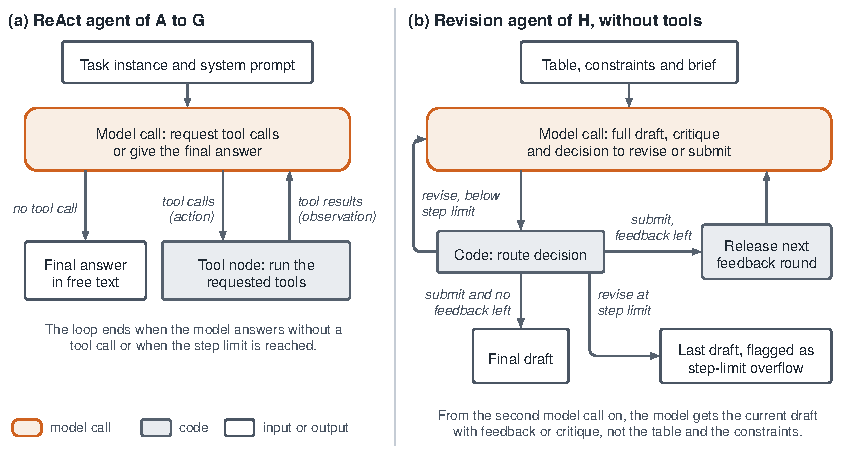
\includegraphics[width=\linewidth]{Figures/fig_agents (1).pdf}
\caption[Control flow of the agents of A to H]{Control flow of the agents of A to H.}
\label{fig:paradigms-agents}
\end{figure}

\begin{figure}[htbp]
\centering
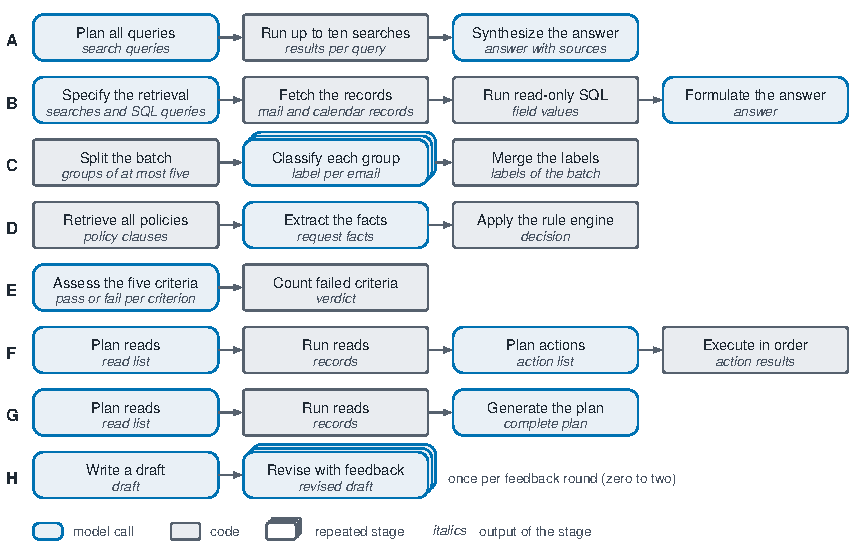
\includegraphics[width=\linewidth]{Figures/fig_workflows.pdf}
\caption[Processing stages of the LLM workflows of A to H]{Processing stages of the LLM workflows of A to H.}
\label{fig:paradigms-workflows}
\end{figure}
\FloatBarrier

The following notes add the implementation details that matter for reading the results.

\paragraph{A. Exploratory research and synthesis.}
\label{app:implementation/a}
The task instances store the reference answer and links to the sources that support it. The LLM workflow groups the search results by query and removes duplicate URLs before the synthesis. Because one model response can request several searches, two agent executions made eleven and fifteen searches despite the recursion limit of 21. The task instances do not rule out that a model knows an answer without searching.

\paragraph{B. Structured data retrieval and transformation.}
\label{app:implementation/b}
The LLM workflow stages the fetched mail and calendar records in temporary tables of its database connection and computes each answer field with read-only SQL; a failing query leaves its field empty. These SQL queries wait for the same synthetic delay as tool calls but are not counted as tool calls. Three agent executions made fifteen, fifteen and seventeen tool calls, so the intended budget of twelve was not a hard cap.

\paragraph{C. Ambiguous classification and disambiguation.}
\label{app:implementation/c}
The group loop runs inside one graph node, so the LLM workflow makes one model call for three or five emails and two for eight. No clean agent execution used the CRM tools.

\paragraph{D. Compliance and rule-based decisioning.}
\label{app:implementation/d}
The LLM workflow retrieves the policy catalogue and every listed document before it extracts the request facts. The rule engine then evaluates the retrieved clauses, so a wrong fact extraction can still lead to a wrong decision. The agent chooses which documents to retrieve.

\paragraph{E. Output verification and quality control.}
\label{app:implementation/e}
The verdict engine maps zero failed criteria to \textit{pass}, one or two to \textit{needs revision} and three or more to \textit{fail}. It stops with an error if the five criteria are not assessed exactly once each, instead of returning a default verdict. No clean agent execution used the CRM tools.

\paragraph{F. Transactional action execution.}
\label{app:implementation/f}
Before each execution, the runner rebuilds the database from the seed records; timing starts afterwards. The backend refuses some case closures under a fixed rule, so a returned refusal can determine the next action. The LLM workflow records failed actions but does not plan again.

\paragraph{G. Strategic and adaptive planning.}
\label{app:implementation/g}
The stored reference plans contain three actions at low, five to seven at medium and fifteen to eighteen at high difficulty; these lengths are not proven optimal. After the execution, a simulator applies the plan to a fresh in-memory copy of the seed records and checks the preconditions of each action and then the goal. A plan with one violated precondition fails as a whole.

\paragraph{H. Content drafting and refinement.}
\label{app:implementation/h}
Because the router checks a submission first, the turn limit in Table~\ref{tab:app-implementations} only stops self-revision. The agent then returns its current draft with an overflow flag.

\subsubsection{Development Decisions}
\label{app:protocol/development}

Task instances and implementations were refined together. The development log records the starting state, decision, result and finding for each iteration. Table~\ref{tab:app-implementation-development} summarizes the decisions needed to understand the retained implementations. The cited IT entries are located in \texttt{docs/iteration\_log.md} in the digital appendix (Appendix~\ref{app:repository}). The table summarizes development evidence; final comparative success rates are reported separately in Section~\ref{subsubsec:TADF/results}.

\begingroup
\renewcommand{\baselinestretch}{1}
\small
\setlength{\tabcolsep}{4pt}
\renewcommand{\arraystretch}{1.08}
\begin{longtable}{>{\raggedright\arraybackslash}p{\dimexpr0.060\linewidth-2\tabcolsep\relax} >{\raggedright\arraybackslash}p{\dimexpr0.280\linewidth-2\tabcolsep\relax} >{\raggedright\arraybackslash}p{\dimexpr0.360\linewidth-2\tabcolsep\relax} >{\raggedright\arraybackslash}p{\dimexpr0.300\linewidth-2\tabcolsep\relax}}
\caption[Development decisions for the implementations]{Development decisions for the implementations.}\label{tab:app-implementation-development} \\
\toprule
\textbf{ID} & \textbf{Starting problem} & \textbf{Development decision} & \textbf{Result and evidence boundary} \\
\midrule
\endfirsthead
\multicolumn{4}{l}{\tablename~\thetable{} (continued)} \\
\toprule
\textbf{ID} & \textbf{Starting problem} & \textbf{Development decision} & \textbf{Result and evidence boundary} \\
\midrule
\endhead
\midrule
\multicolumn{4}{r}{\emph{Continued on the next page.}} \\
\endfoot
\bottomrule
\endlastfoot
A & Familiar facts allowed correct answers without decisive retrieval; compound answers also introduced answer-format effects. & Replace trivia with constructed research questions; distinguish parallel retrieval from linked searches; add checks without tools and single-value endpoints for the high level (IT-031, IT-038, IT-042). & The revised set exercises retrieval dependencies. Checks without tools were used during development, but the stored check lacks model metadata and cannot establish absence of memorization for every model. \\
\addlinespace[2.5pt]
B & Earlier variants mixed retrieval with in-context arithmetic or obscured the intended mail/calendar interfaces. Generated query conventions also caused failures. & Use one retrieval-specification call, tool-based mail/calendar fetching, SQL over CRM and staged records, and one answer call (IT-033, IT-037, IT-043). & The retained implementation separates query construction from deterministic execution. Semantic matching and SQL correctness still depend on the generated specification. \\
\addlinespace[2.5pt]
C & Single-email classification gave little scope for different control behavior. & Construct small email batches and use a fixed chunk size of five in the LLM workflow, retaining the complete batch in the agent context (IT-040, IT-044). & This retains a case where external tools are unnecessary. The tested batches do not establish an advantage for chunking at large context sizes. \\
\addlinespace[2.5pt]
D & With the complete policy inside the prompt, both implementations largely reduced to one model call. & Move policies to a separate registry, add interacting rules and distractors, and separate fact extraction from deterministic policy application (IT-041, IT-045). & The retained contrast concerns applying retrieved rules in code or within the model context. Correct rule execution still requires correctly extracted facts. \\
\addlinespace[2.5pt]
E & The original ranking design was replaced by verdicts; a later version still asked both implementations to apply the complete rubric in one call. & Keep the criterion assessments in one structured model call and move the verdict calculation to code (IT-022, IT-046). & The engine checks criterion coverage and calculates the verdict. The quality of the individual criterion judgments remains model-dependent. \\
\addlinespace[2.5pt]
F & The initial action planner lacked identifiers revealed by reads. Later review found insufficient action-outcome cases and predicates affected by changed seed records. & Add retrieval before action planning; introduce three action-outcome instances; repair predicates and express organizational requirements through runbook excerpts (IT-014, IT-047, IT-049). & Development checks exercised successful actions and prohibited alternatives. The retained LLM workflow can plan from read results but cannot revise its action list during dispatch. The outcome check of f-med-5 was not adjusted to the extended seed and rejects the complete action set (Appendix~\ref{app:results/contrasts}). \\
\addlinespace[2.5pt]
G & Abstract planning tasks did not match the local workplace setting. A later review considered adding further revision or retrieval mechanisms. & Construct CRM scenarios with a plan simulator; retain the two-stage LLM workflow and adaptive retrieval agent, and align the request/runbook wording (IT-023, IT-050, IT-051). & Reference plans and invalid-action cases were tested mechanically. A verifier-driven revision stage was not implemented in the main experimental comparison. \\
\addlinespace[2.5pt]
H & Qualitative ratings alone did not capture violated constraints; early numeric checks rejected valid arithmetic derivations. & Combine deterministic checks with qualitative scoring, permit valid derived numbers, and retain inline data and identical scripted feedback (IT-025--028, IT-052). & Inline data limits retrieval effects. H tests fixed revision stages against model-selected self-revision; judge reliability remains subject to Appendix~\ref{app:protocol/judges}. \\
\end{longtable}
\endgroup

The development checks informed the revisions but did not test the implementations on unused tasks. The main experimental comparison executed the state frozen in IT-053.

\subsubsection{Execution of the Main Experimental Comparison}
\label{app:protocol/execution}

The main experimental comparison ran on 6 and 7 July 2026. It used GPT-5.4-nano, GPT-5.4-mini and GPT-5.2 on the same task instances and implementations; this three-model design replaced the single-model plan of the protocol (D-032, Appendix~\ref{app:protocol/changes}). One batch contains the fifteen task instances of a task archetype, each executed with both orchestration paradigms, which gives thirty executions. The five clean batches per task archetype give forty batches and 1,200 executions. The three models add twenty-four perturbation batches with 252 executions (Appendix~\ref{app:protocol/metrics}).

Table~\ref{tab:app-model-settings} lists the model snapshots, repetitions and reasoning settings. The count in each column applies to one task instance or perturbation variant per orchestration paradigm. All model calls request temperature 0 and seed 42, which did not remove variation between repeated executions. For each model, both orchestration paradigms use the same configuration; the reasoning setting differs between the models.

\begin{table}[htbp]
\centering
\caption[Models and repetitions of the main experimental comparison]{Models and repetitions of the main experimental comparison.}
\label{tab:app-model-settings}
\renewcommand{\baselinestretch}{1}
\small
\setlength{\tabcolsep}{4pt}
\renewcommand{\arraystretch}{1.08}
\begin{tabular}{>{\raggedright\arraybackslash}p{\dimexpr0.380\linewidth-2\tabcolsep\relax} >{\raggedright\arraybackslash}p{\dimexpr0.120\linewidth-2\tabcolsep\relax} >{\raggedright\arraybackslash}p{\dimexpr0.160\linewidth-2\tabcolsep\relax} >{\raggedright\arraybackslash}p{\dimexpr0.340\linewidth-2\tabcolsep\relax}}
\toprule
\textbf{Model snapshot} & \textbf{Clean} & \textbf{Perturbed} & \textbf{Reasoning setting} \\
\midrule
\texttt{gpt-5.4-nano-2026-03-17} & 2 & 1 & Not explicitly set \\
\addlinespace[2.5pt]
\texttt{gpt-5.4-mini-2026-03-17} & 2 & 1 & Not explicitly set \\
\addlinespace[2.5pt]
\texttt{gpt-5.2-2025-12-11} & 1 & 1 & \texttt{reasoning\_effort="none"} \\
\bottomrule
\end{tabular}
\end{table}

The grid runner sets the model and run label for each batch and processes models, runs and task archetypes in a fixed order. The runners of the task archetypes load the task instances, execute both orchestration paradigms, record resource use and apply the outcome checks. The aggregation script combines the result files into one file with 1,452 rows, one per execution, identified by model, run label, task archetype, task instance and orchestration paradigm.

IT-053 records two incidents. A usage limit of the search provider made seven A batches fail: the second GPT-5.4-nano clean batch, both GPT-5.4-mini clean batches, the GPT-5.2 clean batch and the three perturbation batches. Their result files were discarded, and the batches were repeated on 7 July 2026 after a plan upgrade; the first GPT-5.4-nano batch predates the limit and was kept. Provider throttling also lengthened some executions. A request timeout of 300 seconds with three retries was added during the runs, so these client settings were not constant for all batches. The median latency reduces the influence of single long executions but not of the provider conditions.

All other failed executions remain in the data, including recursion-limit failures of the B agent and output-validation failures of the A and F LLM workflows. For GPT-5.4-nano and GPT-5.4-mini, the two clean repetitions give 480 matched combinations of task instance, orchestration paradigm and model, of which 49 changed their task success (10.2 percent). GPT-5.2 ran only one clean repetition, so its repeatability was not measured.

\subsubsection{Design and Execution of the Deep-Dive Runs}
\label{app:protocol/deepdive}

This section documents the deep-dive runs of Section~\ref{subsubsec:TADF/deepdive}. The development log records their planning after the first interpretation of the main experimental comparison (IT-054, IT-055), the construction and execution of the five task families (IT-056 to IT-068) and the confirmation test (IT-069). All task instances were constructed for this study on the local CRM, mail and calendar data. Table~\ref{tab:app-deepdive-design} lists their variants and contrasts.

\begingroup
\renewcommand{\baselinestretch}{1}
\small
\setlength{\tabcolsep}{4pt}
\renewcommand{\arraystretch}{1.08}
\begin{longtable}{>{\raggedright\arraybackslash}p{\dimexpr0.190\linewidth-2\tabcolsep\relax} >{\raggedright\arraybackslash}p{\dimexpr0.170\linewidth-2\tabcolsep\relax} >{\raggedright\arraybackslash}p{\dimexpr0.640\linewidth-2\tabcolsep\relax}}
\caption[Task families and variants of the deep-dive runs]{Task families and variants of the deep-dive runs. Counts refer to task instances, not executions.}\label{tab:app-deepdive-design} \\
\toprule
\textbf{Task family or test} & \textbf{Task instances} & \textbf{Variants and contrasts} \\
\midrule
\endfirsthead
\multicolumn{3}{l}{\tablename~\thetable{} (continued)} \\
\toprule
\textbf{Task family or test} & \textbf{Task instances} & \textbf{Variants and contrasts} \\
\midrule
\endhead
\midrule
\multicolumn{3}{r}{\emph{Continued on the next page.}} \\
\endfoot
\bottomrule
\endlastfoot
P: Plan uncertainty & 20: four variants, five each & P-a: a read determines the number of actions. P-b: the outcomes of earlier actions determine it. P-c: a needed fact lies in the CRM, mail or calendar system, and the task does not name which. P-d: record values determine the order of actions. \\
\addlinespace[2.5pt]
X: Crossed gates & 15: three variants, five each & X-1: written rules applied to the outcomes of closing attempts. X-2: a two-step retrieval chain followed by updates with record-specific values. X-3: written rules, decidable before any action, that require different updates for different records. \\
\addlinespace[2.5pt]
L: Payload scaling & 18: three task shapes, three volumes, two each & L-1: raising the longest-open case. L-2: a uniform bulk update. L-3: finding the oldest email on a topic. The records grow by factors of 1, 5 and 20, from 8 to 160 cases or from 10 to 200 emails, under fixed instruction templates. In the bulk update, the number of actions also grows, from 2 to 40. \\
\addlinespace[2.5pt]
M: State drift & 15: three variants, five each & M-1: a change during the execution that the next tool response reveals. M-2: a change after which an outdated write succeeds without a signal. M-3: as M-2, with an instruction to re-check records before each change. \\
\addlinespace[2.5pt]
S: Staged adaptivity & 15: ten reused, five new & S-1: the five X-1 instances. S-2: the five P-b instances. S-3: five new instances that add a report on the cases closed in the same execution; one of them involves no refusal and serves as a control. \\
\addlinespace[2.5pt]
Confirmation test & Two F instances & Target: reassigning the nine cases of one agent, two of them closed, to another agent (f-med-3). Control: moving seventeen opportunities to another stage (f-med-4). \\
\end{longtable}
\endgroup

\paragraph{Implementations and conditions.}
P, X, L and M reused the LLM workflow and the agent of F without changes (Appendix~\ref{app:implementation/f}). Both orchestration paradigms received the same instruction, including its runbook excerpt. In X, the models applied the written rules themselves; the deterministic rule engine of D was not added. Before each execution, the runner restored the database from the seed data. L then inserted the additional records of the task instance, and M installed its trigger. The trigger closes a second record as soon as the execution first changes a watched record, not after a fixed time. Both orchestration paradigms thus meet the change at the same point of the task, and M does not examine changes before the first write. In M-1, the trigger works in both directions, so the check accepts either order of the two closing operations.

S added a state-machine LLM workflow that keeps the read stage of F. One model call plans each closing step with branches for the three outcomes of the closing tool: closed, refused and already closed. During the execution, code selects the matching branch and inserts only the case identifier and the stated reason into prepared texts. It stops after at most twelve steps and at outcomes without a planned branch. Actions after the last step, such as a final report, receive no inserted values, so their content is fixed when the plan is made. Before the S runs, the log states three hypotheses: the state-machine LLM workflow solves S-1 and S-2 but not S-3, which the agent solves. For the ten reused task instances, only the state-machine LLM workflow was executed; the observations of the LLM workflow and the agent come from X-1 and P-b. The five new task instances were executed with all three implementations.

The map-form LLM workflow of the confirmation test also keeps the read stage of F. A model call lists the items of the task. Code then requests a separate action plan for each item, for at most forty items, and executes it. The comparison uses the GPT-5.2 executions of the original LLM workflow and the agent from the main experimental comparison. Before the test, the log states two hypotheses: the map-form LLM workflow solves the target, and the control remains solved. The log entries IT-049 and IT-069 and the docstrings of the implementation describe the target as nine updates with item-specific owners and notes. The stored task instance and its outcome check, however, require the same new agent for all nine cases. The test therefore examined the complete processing of a list of records with one model call per item, not the binding of different values to different items. IT-083 records this correction and its consequence for the framework (Section~\ref{subsubsec:TADF/evidence}).

\paragraph{Execution and record selection.}
The standard runs of the five task families used the models and settings of the main experimental comparison (Appendix~\ref{app:protocol/execution}) in five model/run configurations: two repetitions each for GPT-5.4-nano and GPT-5.4-mini and one for GPT-5.2. They took place from 16 to 22 July 2026 and contain 805 new executions: 200 for P, 150 for X, 180 for L, 150 for M and 125 for S. S also reuses 100 observations from X-1 and P-b, which are not new executions. Because GPT-5.2 had only one repetition, a supplementary GPT-5.2 repetition of P-c added ten executions on 22 July 2026. The confirmation test on 3 August 2026 comprises two GPT-5.2 executions on each of its two task instances and one preliminary GPT-5.4-nano execution on the target. Preliminary runs of the families are stored separately and excluded from the comparisons. The result files under \path{data/results/phase2b/} record the model, run label, task family, task instance and implementation. After a re-execution, the analysis keeps the latest observation for each combination of these identifiers. Executions that ended with an exception count as unsuccessful and have no token record; this applies to 26 of the 805.

\paragraph{Checks and corrections.}
Each construction script tests every outcome check twice: it must fail on the unchanged initial state and pass after the specified correct actions. Before the standard runs, one outcome check of P and the instructions of the state-machine LLM workflow were adjusted (IT-056, IT-067). During the runs, the expected result of one P-d instance, the mail search and the closing tool were corrected for both orchestration paradigms (IT-057, IT-062, IT-064). The affected P-d instance, the six L email instances and the five M-1 instances were executed again. All runs of P and X, including the repeated P-d instance, preceded the two tool corrections and were not repeated after them; of P-c, only the supplementary GPT-5.2 repetition ran afterwards.

The repository contains the construction scripts and runners, both additional LLM workflows, the analysis notebook of the deep-dive runs and the development log (Appendix~\ref{app:repository}).

\subsubsection{Protocol and Implemented Procedure}
\label{app:protocol/changes}

The experimental protocol was written before the task archetypes were implemented (IT-001, IT-002). It specified the compared conditions, the task corpus, the tool infrastructure, the execution procedure, the metrics and the statistical analysis. It was not registered publicly. Deviations during development were recorded as D-001 to D-032. The protocol lists 20 of them; the other twelve appear only in the development log. Several deviations were also written into the protocol text, for example the local database (D-001), the hash-based delays (D-005) and the deterministic checks of E and G (D-011, D-012). Table~\ref{tab:app-protocol-changes} lists where the implemented procedure still differs from the protocol or from later plans in the development log. Where plans and records differ, the code and result files describe what was executed. The repository contains the protocol in its last version (Appendix~\ref{app:repository}).

\begingroup
\renewcommand{\baselinestretch}{1}
\small
\setlength{\tabcolsep}{4pt}
\renewcommand{\arraystretch}{1.08}
\begin{longtable}{>{\raggedright\arraybackslash}p{\dimexpr0.170\linewidth-2\tabcolsep\relax} >{\raggedright\arraybackslash}p{\dimexpr0.320\linewidth-2\tabcolsep\relax} >{\raggedright\arraybackslash}p{\dimexpr0.380\linewidth-2\tabcolsep\relax} >{\raggedright\arraybackslash}p{\dimexpr0.130\linewidth-2\tabcolsep\relax}}
\caption[Differences between the planned and the implemented procedure]{Differences between the planned and the implemented procedure. \emph{Planned} refers to the protocol or, where named, to a later plan in the development log. \emph{Record} names the deviation (D) or log entry (IT); a dash marks a difference that was identified only when this thesis was written.}\label{tab:app-protocol-changes} \\
\toprule
\textbf{Aspect} & \textbf{Planned} & \textbf{Implemented} & \textbf{Record} \\
\midrule
\endfirsthead
\multicolumn{4}{l}{\tablename~\thetable{} (continued)} \\
\toprule
\textbf{Aspect} & \textbf{Planned} & \textbf{Implemented} & \textbf{Record} \\
\midrule
\endhead
\midrule
\multicolumn{4}{r}{\emph{Continued on the next page.}} \\
\endfoot
\bottomrule
\endlastfoot
Conditions & Always LLM workflow, Always agent, a difficulty-only router and a TADF router; the routers select between recorded executions. & Only the two orchestration paradigms were executed; no difficulty-only router was built. Routing was examined retrospectively (Section~\ref{subsubsec:TADF/functionality}) and on WorkBench (Section~\ref{subsubsec:TADF/episode2}). & -- \\
\addlinespace[2.5pt]
Models and repetitions & One model, GPT-5.2; one execution per task instance and orchestration paradigm; 240 plus 48 perturbation executions. & Three models; two clean repetitions each for GPT-5.4-nano and GPT-5.4-mini, one for GPT-5.2; 1,200 clean plus 252 perturbation executions. & D-032 \\
\addlinespace[2.5pt]
Task instances & Taken from benchmark sources with their original meaning; own construction only where no source fits. & All 120 constructed for this study; benchmark sources supplied task patterns (Appendix~\ref{app:taxonomy/sources}). & e.g.\ D-012, D-016 \\
\addlinespace[2.5pt]
Reasoning setting & \texttt{reasoning\_effort} set to \texttt{"none"} for all executions. & Set only for GPT-5.2; provider default for the GPT-5.4 models. & IT-053 \\
\addlinespace[2.5pt]
Step limits & One per task archetype, e.g.\ 2/6/10 steps in F and 5/12/25 in G; exceeding it counts as failure. & For the agents of A, B, C, G and H; no task-specific limit for the agents of D, E and F. & D-007, D-012 \\
\addlinespace[2.5pt]
Workflow nodes & At most one model call per graph node. & In C, one node classifies all groups of a batch, with two model calls for eight emails. & IT-044 \\
\addlinespace[2.5pt]
Database reset & Seed state restored before each execution. & Restored before each F execution only. F alone changes the database; the other task archetypes read the state left by the preceding F execution. & -- \\
\addlinespace[2.5pt]
Success in A & Quality score from a rubric-based judgment against the expected answer. & Binary judge decision whether the answer states the reference fact. & IT-008 \\
\addlinespace[2.5pt]
Success in H & Judge quality score as primary measure; deterministic checks reported alongside (D-013). & Solved if all deterministic checks pass; judge quality score complementary. & -- \\
\addlinespace[2.5pt]
Judge agreement & Weighted $\kappa\geq0.6$ on a human-rated 20 percent sample; if missed, judge ratings discarded and a second human reviewer rates. & A: $\kappa=1.000$. H: $\kappa=0.348$; judge score kept as complementary measure, AC1 reported, no second reviewer. & D-015 \\
\addlinespace[2.5pt]
Judge model & Fixed GPT-5.2 judge for all models (IT-053). & Model of the judged execution; no separate judge model recorded. & -- \\
\addlinespace[2.5pt]
Error rate & Share of executions ending with incorrect output or iteration overflow. & Share with a recorded error or iteration overflow; incorrect output counts only as failed task success. & -- \\
\addlinespace[2.5pt]
Robustness & Relative drop in success on a 20 percent subset with synonyms and irrelevant sentences; IT-053: only base tasks solved in all clean executions of a model. & Success rate on 42 fixed variants (35 percent of the task instances) with varied wording changes, without this restriction. & -- \\
\addlinespace[2.5pt]
Analysis & Per task archetype and difficulty level: paired Wilcoxon tests, Cliff's delta with bootstrap intervals and Holm correction; an equally weighted aggregate score; an efficiency frontier. & Descriptive rates and resource summaries. The planned tests, effect sizes and efficiency frontier were computed afterwards, when this thesis was written (\path{statistical_analysis.ipynb}). No combination reaches $p<0.05$; for five pairs, the exact two-sided Wilcoxon $p$-value is at least 0.0625. The aggregate score was not computed, because the protocol left its normalization open. & -- \\
\addlinespace[2.5pt]
Deep-dive runs & Not planned. & Five task families and a confirmation test after the main experimental comparison for questions it left open (Section~\ref{subsubsec:TADF/deepdive}). & IT-054 to IT-069 \\
\end{longtable}
\endgroup

% Appendix D: Detailed Experimental Results

\subsection{Detailed Experimental Results}
\label{app:results}

This appendix contains the detailed tables for Section~\ref{subsubsec:TADF/results}. D.1 and D.2 cover the main experimental comparison, and D.3 and D.4 the deep-dive runs. The notebook \path{statistical_analysis.ipynb} reproduces each table of Section~\ref{subsubsec:TADF/results} and of this appendix from the stored result files and prints it under its label (Appendix~\ref{app:repository}). Counts give successful executions over all executions of the stated group. Token values use the executions with a token record; missing records are not treated as zero. W denotes the LLM workflow, and the letters A--H denote the task archetypes as in Table~\ref{tab:grid-results}.

\subsubsection{Main Experimental Comparison}
\label{app:results/main}

Table~\ref{tab:app-intervals} reports the differences between the orchestration paradigms with their uncertainty. The intervals are 95 percent percentile bootstrap intervals over task instances with 10,000 resamples, so the repeated executions of a task instance stay together. The exact sign-flip test compares the mean difference over the 15 task instances with all sign assignments, and Holm's correction covers the eight task archetypes. The notebook also gives the intervals for each model.

\begin{table}[htbp]
\centering
\caption[Success differences and token ratios with 95 percent intervals]{Success differences and token ratios with 95 percent intervals.}
\label{tab:app-intervals}
\renewcommand{\baselinestretch}{1}
\footnotesize
\setlength{\tabcolsep}{3pt}
\renewcommand{\arraystretch}{1.08}
\begin{tabular*}{\linewidth}{@{\extracolsep{\fill}}l c c c c@{}}
\toprule
\textbf{ID} & \textbf{Success, W $-$ Agent (pp)} & \textbf{Sign-flip $p$} & \textbf{Holm $p$} & \textbf{Token cost, Agent/W} \\
\midrule
A & $-$10.7 [$-$25.3, 4.0] & 0.254 & 1.000 & 2.03 [1.26, 2.86] \\
B & $-$12.0 [$-$32.0, 5.3] & 0.313 & 1.000 & 7.91 [4.17, 12.49] \\
C & $-$2.7 [$-$8.0, 0.0] & 1.000 & 1.000 & 0.85 [0.76, 0.95] \\
D & 20.0 [9.3, 32.0] & 0.008 & 0.063 & 6.16 [6.15, 6.17] \\
E & 8.0 [$-$6.7, 21.4] & 0.391 & 1.000 & 0.90 [0.89, 0.90] \\
F & $-$26.7 [$-$48.0, $-$8.0] & 0.047 & 0.281 & 4.34 [2.78, 6.40] \\
G & $-$13.3 [$-$36.0, 8.0] & 0.324 & 1.000 & 2.89 [2.28, 3.59] \\
H & 14.7 [5.3, 26.7] & 0.031 & 0.219 & 1.49 [1.32, 1.72] \\
\bottomrule
\end{tabular*}
\par\smallskip
\begin{minipage}{\linewidth}\footnotesize
pp: percentage points; brackets: 95 percent intervals. Token cost, Agent/W: the agent's mean token cost divided by the LLM workflow's.
\end{minipage}
\end{table}

Table~\ref{tab:app-token-results} relates token cost to success. Tokens per success divide the recorded tokens of all executions, including unsuccessful ones, by the number of successful executions. Executions without a token record add no tokens, so the values of the LLM workflow in A and F and of the agent in B are slightly too low. The median of the eight ratios is 2.21.

\begin{table}[htbp]
\centering
\caption[Token cost per successful execution]{Token cost per successful execution.}
\label{tab:app-token-results}
\renewcommand{\baselinestretch}{1}
\footnotesize
\setlength{\tabcolsep}{3pt}
\renewcommand{\arraystretch}{1.08}
\begin{tabular}{>{\raggedright\arraybackslash}p{\dimexpr0.12\linewidth-2\tabcolsep\relax} *{8}{>{\raggedleft\arraybackslash}p{\dimexpr0.11\linewidth-2\tabcolsep\relax}}}
\toprule
 & \textbf{A} & \textbf{B} & \textbf{C} & \textbf{D} & \textbf{E} & \textbf{F} & \textbf{G} & \textbf{H} \\
\midrule
W & 7,547 & 3,197 & 1,713 & 903 & 1,725 & 8,389 & 5,891 & 3,214 \\
Agent & 13,555 & 20,515 & 1,415 & 6,953 & 1,722 & 23,471 & 13,996 & 6,592 \\
Agent/W & 1.80 & 6.42 & 0.83 & 7.70 & 1.00 & 2.80 & 2.38 & 2.05 \\
\bottomrule
\end{tabular}
\end{table}

Table~\ref{tab:app-robustness-results} reports task success on the perturbation variants: fifteen executions per orchestration paradigm, eighteen in D and G. Because not all base task instances were solved in every clean execution, these rates combine baseline difficulty with sensitivity to the changed wording (Appendix~\ref{app:protocol/metrics}).

\begin{table}[htbp]
\centering
\caption[Task success on the perturbation variants]{Task success on the perturbation variants.}
\label{tab:app-robustness-results}
\renewcommand{\baselinestretch}{1}
\footnotesize
\setlength{\tabcolsep}{3pt}
\renewcommand{\arraystretch}{1.08}
\begin{tabular}{>{\raggedright\arraybackslash}p{\dimexpr0.12\linewidth-2\tabcolsep\relax} *{8}{>{\raggedleft\arraybackslash}p{\dimexpr0.11\linewidth-2\tabcolsep\relax}}}
\toprule
 & \textbf{A} & \textbf{B} & \textbf{C} & \textbf{D} & \textbf{E} & \textbf{F} & \textbf{G} & \textbf{H} \\
\midrule
W & 12/15 & 13/15 & 15/15 & 18/18 & 15/15 & 13/15 & 17/18 & 13/15 \\
Agent & 13/15 & 15/15 & 15/15 & 13/18 & 14/15 & 15/15 & 16/18 & 13/15 \\
\bottomrule
\end{tabular}
\end{table}

Most failures carried no error signal. Seven of the 1,200 executions ended with a recorded error or step-limit overflow; all others returned a result, which the outcome check accepted or rejected. In D, the LLM workflow returned the reference decision in all 75 executions. Twelve of the agent's fifteen incorrect decisions were less restrictive than the reference: seven escalations instead of a decline, four approvals instead of an escalation and one lower escalation level. In E, the criterion assessments of the LLM workflow in its 90 scored clean and perturbation executions contained 35 false fails, which mark a satisfied criterion as failed, and 17 missed fails, which overlook a failed criterion.
\FloatBarrier

\subsubsection{Difficulty Levels and Task Requirements}
\label{app:results/contrasts}

Table~\ref{tab:app-difficulty-results} reports task success by difficulty level. The levels are defined per task archetype (Table~\ref{tab:app-difficulty}) and form no common scale. Table~\ref{tab:app-high-model-results} separates the high level by model.

\begin{table}[htbp]
\centering
\caption[Task success by difficulty level]{Task success by difficulty level.}
\label{tab:app-difficulty-results}
\renewcommand{\baselinestretch}{1}
\footnotesize
\setlength{\tabcolsep}{3pt}
\renewcommand{\arraystretch}{1.08}
\begin{tabular}{>{\raggedright\arraybackslash}p{\dimexpr0.064\linewidth-2\tabcolsep\relax} >{\raggedright\arraybackslash}p{\dimexpr0.306\linewidth-2\tabcolsep\relax} *{6}{>{\centering\arraybackslash}p{\dimexpr0.105\linewidth-2\tabcolsep\relax}}}
\toprule
 & & \multicolumn{2}{c}{\textbf{Low}} & \multicolumn{2}{c}{\textbf{Medium}} & \multicolumn{2}{c}{\textbf{High}} \\
\cmidrule(lr){3-4}\cmidrule(lr){5-6}\cmidrule(lr){7-8}
\textbf{ID} & \textbf{Varied demand} & \textbf{W} & \textbf{Agent} & \textbf{W} & \textbf{Agent} & \textbf{W} & \textbf{Agent} \\
\midrule
A & Sources, search chain & 21/25 & 19/25 & 19/25 & 20/25 & 14/25 & 23/25 \\
B & Systems combined & 25/25 & 25/25 & 16/25 & 23/25 & 8/25 & 10/25 \\
C & Ambiguity, batch size & 25/25 & 25/25 & 23/25 & 25/25 & 25/25 & 25/25 \\
D & Rule interaction & 25/25 & 22/25 & 25/25 & 18/25 & 25/25 & 20/25 \\
E & Subtlety of failures & 21/25 & 20/25 & 19/25 & 17/25 & 19/25 & 16/25 \\
F & Action scope, dependence & 20/25 & 20/25 & 13/25 & 20/25 & 2/25 & 15/25 \\
G & Plan length & 16/25 & 22/25 & 19/25 & 20/25 & 11/25 & 14/25 \\
H & Constraints, feedback & 21/25 & 20/25 & 18/25 & 9/25 & 1/25 & 0/25 \\
\bottomrule
\end{tabular}
\end{table}

\begin{table}[htbp]
\centering
\caption[Task success at the high difficulty level by model]{Task success at the high difficulty level by model.}
\label{tab:app-high-model-results}
\renewcommand{\baselinestretch}{1}
\footnotesize
\setlength{\tabcolsep}{3pt}
\renewcommand{\arraystretch}{1.08}
\begin{tabular}{>{\raggedright\arraybackslash}p{\dimexpr0.064\linewidth-2\tabcolsep\relax} *{6}{>{\centering\arraybackslash}p{\dimexpr0.156\linewidth-2\tabcolsep\relax}}}
\toprule
 & \multicolumn{2}{c}{\textbf{GPT-5.4-nano}} & \multicolumn{2}{c}{\textbf{GPT-5.4-mini}} & \multicolumn{2}{c}{\textbf{GPT-5.2}} \\
\cmidrule(lr){2-3}\cmidrule(lr){4-5}\cmidrule(lr){6-7}
\textbf{ID} & \textbf{W} & \textbf{Agent} & \textbf{W} & \textbf{Agent} & \textbf{W} & \textbf{Agent} \\
\midrule
A & 3/10 & 9/10 & 7/10 & 9/10 & 4/5 & 5/5 \\
B & 3/10 & 5/10 & 5/10 & 2/10 & 0/5 & 3/5 \\
C & 10/10 & 10/10 & 10/10 & 10/10 & 5/5 & 5/5 \\
D & 10/10 & 8/10 & 10/10 & 8/10 & 5/5 & 4/5 \\
E & 5/10 & 7/10 & 9/10 & 5/10 & 5/5 & 4/5 \\
F & 1/10 & 4/10 & 0/10 & 7/10 & 1/5 & 4/5 \\
G & 2/10 & 3/10 & 6/10 & 7/10 & 3/5 & 4/5 \\
H & 0/10 & 0/10 & 0/10 & 0/10 & 1/5 & 0/5 \\
\bottomrule
\end{tabular}
\end{table}

Table~\ref{tab:app-main-contrasts} lists the fifteen task instances of F. In f-high-1, f-high-2 and f-high-5, a later action depends on the outcome of an earlier one. In f-low-2, the closing tool refuses the case with the message that an automatic close is not permitted, while the outcome check expects the status `Closed'. All its executions stopped after the refusal, and the agents reported it.

\begin{table}[htbp]
\centering
\caption[Task success in action execution (F) by task instance]{Task success in action execution (F) by task instance.}
\label{tab:app-main-contrasts}
\renewcommand{\baselinestretch}{1}
\footnotesize
\setlength{\tabcolsep}{4pt}
\renewcommand{\arraystretch}{1.08}
\begin{tabular}{>{\raggedright\arraybackslash}p{\dimexpr0.13\linewidth-2\tabcolsep\relax} >{\raggedright\arraybackslash}p{\dimexpr0.67\linewidth-2\tabcolsep\relax} >{\centering\arraybackslash}p{\dimexpr0.1\linewidth-2\tabcolsep\relax} >{\centering\arraybackslash}p{\dimexpr0.1\linewidth-2\tabcolsep\relax}}
\toprule
\textbf{Instance} & \textbf{Required actions} & \textbf{W} & \textbf{Agent} \\
\midrule
f-low-1 & Send one email with given recipient, subject and body & 5/5 & 5/5 \\
f-low-2 & Set one case to `Closed'; the closing tool refuses it & 0/5 & 0/5 \\
f-low-3 & Create one calendar event with all details given & 5/5 & 5/5 \\
f-low-4 & Delete one email by its identifier & 5/5 & 5/5 \\
f-low-5 & Change the priority of one case & 5/5 & 5/5 \\
f-med-1 & Set the four open cases of one agent to `In Progress' & 5/5 & 5/5 \\
f-med-2 & Book one call; a calendar read decides the time slot & 1/5 & 5/5 \\
f-med-3 & Reassign the nine cases of one agent, two of them closed & 2/5 & 5/5 \\
f-med-4 & Move seventeen opportunities to another stage & 5/5 & 5/5 \\
f-med-5\textsuperscript{a} & Email the primary contact of every account in one region & 0/5 & 0/5 \\
f-high-1 & Close two cases; each closing outcome selects its email & 0/5 & 3/5 \\
f-high-2 & Close a duplicate case; if refused, change nothing and escalate & 0/5 & 5/5 \\
f-high-3 & Invite the primary contacts of accounts with won opportunities in a region & 2/5 & 1/5 \\
f-high-4 & Email the agent with the most open cases in one team & 0/5 & 1/5 \\
f-high-5 & Close a case; the customer email depends on the outcome & 0/5 & 5/5 \\
\midrule
\multicolumn{2}{l}{Outcome-dependent task instances: f-high-1, f-high-2, f-high-5} & 0/15 & 13/15 \\
\multicolumn{2}{l}{Other twelve task instances} & 35/60 & 42/60 \\
\bottomrule
\end{tabular}
\par\smallskip
\begin{minipage}{\linewidth}\footnotesize
\textsuperscript{a}\,The outcome check cannot be met with the seed used in the runs; see the text.
\end{minipage}
\end{table}

The outcome check of f-med-5 cannot be met. It lists the primary contacts of seven accounts in the named region and rejects emails to any other recipient. Before the main experimental comparison, the named-customer data of B's retrieval tasks added an eighth account in this region to the shared seed (IT-035). IT-047 later repaired other checks affected by this extension, but not this one. An execution that emails all eight primary contacts therefore counts as a failure; the notebook reproduces this with the stored seed. All five agent executions and two LLM-workflow executions sent eight emails; the result files do not record the recipients. The results of f-med-5 therefore do not measure task success. Without f-med-5, F's counts are 35/70 for the LLM workflow and 55/70 for the agent. The sign-flip test is unchanged, because both orchestration paradigms failed all executions of f-med-5. The same extension added a seventeenth opportunity in the stage of f-med-4, whose check derives its targets from the seed. It also added two accounts with won opportunities in the region of f-high-3. This check requires the six original accounts and accepts events for further accounts, so it accepts complete executions but would also accept executions that omit the two added accounts.
\FloatBarrier

\subsubsection{Deep-Dive Task Families}
\label{app:results/deepdive}

The deep-dive runs used five standard model/run configurations: two repetitions each with GPT-5.4-nano and GPT-5.4-mini and one with GPT-5.2 (Appendix~\ref{app:protocol/deepdive}). Table~\ref{tab:app-deep-model-results} separates them by model. Each variant in P, X, M and S has five task instances, each task shape in L six.

\begin{table}[htbp]
\centering
\caption[Task success in the deep-dive runs by model]{Task success in the deep-dive runs by model.}
\label{tab:app-deep-model-results}
\renewcommand{\baselinestretch}{1}
\footnotesize
\setlength{\tabcolsep}{3pt}
\renewcommand{\arraystretch}{1.08}
\begin{tabular}{>{\raggedright\arraybackslash}p{\dimexpr0.11\linewidth-2\tabcolsep\relax} *{9}{>{\centering\arraybackslash}p{\dimexpr0.0988\linewidth-2\tabcolsep\relax}}}
\toprule
 & \multicolumn{3}{c}{\textbf{GPT-5.4-nano}} & \multicolumn{3}{c}{\textbf{GPT-5.4-mini}} & \multicolumn{3}{c}{\textbf{GPT-5.2}} \\
\cmidrule(lr){2-4}\cmidrule(lr){5-7}\cmidrule(lr){8-10}
\textbf{Variant} & \textbf{W} & \textbf{Agent} & \textbf{SM} & \textbf{W} & \textbf{Agent} & \textbf{SM} & \textbf{W} & \textbf{Agent} & \textbf{SM} \\
\midrule
P-a & 10/10 & 10/10 & -- & 10/10 & 10/10 & -- & 5/5 & 5/5 & -- \\
P-b & 0/10 & 7/10 & -- & 0/10 & 3/10 & -- & 0/5 & 5/5 & -- \\
P-c & 3/10 & 10/10 & -- & 6/10 & 10/10 & -- & 3/5 & 4/5 & -- \\
P-d & 3/10 & 5/10 & -- & 6/10 & 7/10 & -- & 5/5 & 5/5 & -- \\
X-1 & 0/10 & 9/10 & -- & 0/10 & 10/10 & -- & 0/5 & 5/5 & -- \\
X-2 & 0/10 & 10/10 & -- & 0/10 & 9/10 & -- & 0/5 & 5/5 & -- \\
X-3 & 1/10 & 4/10 & -- & 4/10 & 10/10 & -- & 5/5 & 5/5 & -- \\
L-1 & 11/12 & 12/12 & -- & 12/12 & 12/12 & -- & 6/6 & 6/6 & -- \\
L-2 & 11/12 & 12/12 & -- & 12/12 & 12/12 & -- & 6/6 & 6/6 & -- \\
L-3 & 11/12 & 12/12 & -- & 11/12 & 12/12 & -- & 6/6 & 6/6 & -- \\
M-1 & 0/10 & 10/10 & -- & 0/10 & 10/10 & -- & 0/5 & 5/5 & -- \\
M-2 & 0/10 & 0/10 & -- & 0/10 & 0/10 & -- & 0/5 & 0/5 & -- \\
M-3 & 0/10 & 5/10 & -- & 0/10 & 6/10 & -- & 0/5 & 5/5 & -- \\
S-1 & 0/10 & 9/10 & 9/10 & 0/10 & 10/10 & 5/10 & 0/5 & 5/5 & 5/5 \\
S-2 & 0/10 & 7/10 & 4/10 & 0/10 & 3/10 & 5/10 & 0/5 & 5/5 & 5/5 \\
S-3 & 0/10 & 5/10 & 1/10 & 1/10 & 4/10 & 1/10 & 1/5 & 4/5 & 2/5 \\
\bottomrule
\end{tabular}
\par\smallskip
\begin{minipage}{\linewidth}\footnotesize
W: original LLM workflow; SM: state-machine LLM workflow; a dash marks an implementation that was not executed. Table~\ref{tab:deepdive-results} describes the variants.
\end{minipage}
\end{table}

Table~\ref{tab:app-family-results} reports the mean token cost. Token records are missing for 26 of the 805 standard executions, which ended with an exception and count as unsuccessful. Superscripts give the number of records where it is smaller than the number of executions. The ratios compare recorded means. In S-1, six unsuccessful executions of the state-machine LLM workflow have no record, so its mean rests on nineteen executions.

\begin{table}[htbp]
\centering
\caption[Token cost in the deep-dive runs]{Token cost in the deep-dive runs.}
\label{tab:app-family-results}
\renewcommand{\baselinestretch}{1}
\footnotesize
\setlength{\tabcolsep}{4pt}
\renewcommand{\arraystretch}{1.08}
\begin{tabular}{>{\raggedright\arraybackslash}p{\dimexpr0.12\linewidth-2\tabcolsep\relax} *{3}{>{\raggedleft\arraybackslash}p{\dimexpr0.18\linewidth-2\tabcolsep\relax}} *{2}{>{\centering\arraybackslash}p{\dimexpr0.17\linewidth-2\tabcolsep\relax}}}
\toprule
 & \multicolumn{3}{c}{\textbf{Mean token cost}} & \multicolumn{2}{c}{\textbf{Ratio}} \\
\cmidrule(lr){2-4}\cmidrule(lr){5-6}
\textbf{Variant} & \textbf{W} & \textbf{Agent} & \textbf{SM} & \textbf{Agent/W} & \textbf{SM/Agent} \\
\midrule
P-a & 3,346 & 9,393 & -- & 2.81 & -- \\
P-b & 4,084\textsuperscript{[24]} & 19,099 & -- & 4.68 & -- \\
P-c & 4,534\textsuperscript{[24]} & 13,335 & -- & 2.94 & -- \\
P-d & 4,177 & 29,723 & -- & 7.12 & -- \\
X-1 & 4,074\textsuperscript{[20]} & 14,356 & -- & 3.52 & -- \\
X-2 & 3,664\textsuperscript{[24]} & 13,790 & -- & 3.76 & -- \\
X-3 & 3,768 & 11,122 & -- & 2.95 & -- \\
L-1 & 4,924 & 16,461 & -- & 3.34 & -- \\
L-2 & 5,414 & 12,555 & -- & 2.32 & -- \\
L-3 & 9,857 & 22,504 & -- & 2.28 & -- \\
M-1 & 3,754\textsuperscript{[17]} & 14,042 & -- & 3.74 & -- \\
M-2 & 3,390\textsuperscript{[24]} & 20,647 & -- & 6.09 & -- \\
M-3 & 3,522 & 13,140 & -- & 3.73 & -- \\
S-1 & 4,074\textsuperscript{[20]} & 14,356 & 5,004\textsuperscript{[19]} & 3.52 & 0.35 \\
S-2 & 4,084\textsuperscript{[24]} & 19,099 & 5,202 & 4.68 & 0.27 \\
S-3 & 4,363\textsuperscript{[23]} & 18,204\textsuperscript{[24]} & 5,255 & 4.17 & 0.29 \\
\bottomrule
\end{tabular}
\end{table}

Table~\ref{tab:app-payload-results} separates L by record volume. Token cost rose with volume in each task shape for both orchestration paradigms. The agent's cost rose by more tokens in all three task shapes, but by a larger factor only in L-1. In L-2, the number of actions also grows with volume. Token counts accumulate over the model calls of an execution, so they do not measure the largest context of a single call.

\begin{table}[htbp]
\centering
\caption[Payload scaling in L by record volume]{Payload scaling in L by record volume.}
\label{tab:app-payload-results}
\renewcommand{\baselinestretch}{1}
\footnotesize
\setlength{\tabcolsep}{4pt}
\renewcommand{\arraystretch}{1.08}
\begin{tabular}{>{\raggedright\arraybackslash}p{\dimexpr0.16\linewidth-2\tabcolsep\relax} >{\centering\arraybackslash}p{\dimexpr0.12\linewidth-2\tabcolsep\relax} *{2}{>{\centering\arraybackslash}p{\dimexpr0.16\linewidth-2\tabcolsep\relax}} *{2}{>{\raggedleft\arraybackslash}p{\dimexpr0.2\linewidth-2\tabcolsep\relax}}}
\toprule
 & & \multicolumn{2}{c}{\textbf{Task success}} & \multicolumn{2}{c}{\textbf{Mean token cost}} \\
\cmidrule(lr){3-4}\cmidrule(lr){5-6}
\textbf{Task shape} & \textbf{Volume} & \textbf{W} & \textbf{Agent} & \textbf{W} & \textbf{Agent} \\
\midrule
L-1 & $\times$1 & 10/10 & 10/10 & 3,259 & 9,366 \\
L-1 & $\times$5 & 10/10 & 10/10 & 4,153 & 12,737 \\
L-1 & $\times$20 & 9/10 & 10/10 & 7,360 & 27,281 \\
\addlinespace[2.5pt]
L-2 & $\times$1 & 10/10 & 10/10 & 3,173 & 8,822 \\
L-2 & $\times$5 & 10/10 & 10/10 & 4,224 & 11,166 \\
L-2 & $\times$20 & 9/10 & 10/10 & 8,844 & 17,678 \\
\addlinespace[2.5pt]
L-3 & $\times$1 & 9/10 & 10/10 & 3,730 & 10,219 \\
L-3 & $\times$5 & 9/10 & 10/10 & 7,066 & 16,705 \\
L-3 & $\times$20 & 10/10 & 10/10 & 18,774 & 40,590 \\
\bottomrule
\end{tabular}
\par\smallskip
\begin{minipage}{\linewidth}\footnotesize
Two task instances per row, executed in the five standard configurations. L-1: raise the longest-open case; L-2: uniform bulk update; L-3: find the oldest email on a topic.
\end{minipage}
\end{table}
\FloatBarrier

\subsubsection{Supplementary Observations and Confirmation Test}
\label{app:results/supplementary}

Table~\ref{tab:app-p-recheck} compares the standard GPT-5.2 repetition of P-c with the supplementary one. Across both repetitions, the LLM workflow solved 5 of 10 executions and the agent 9 of 10. The standard repetition ran before the correction of the mail search, the supplementary one after it (Appendix~\ref{app:protocol/deepdive}). The supplementary executions are not part of the standard counts and token means.

\begin{table}[htbp]
\centering
\caption[Supplementary GPT-5.2 repetition of P-c]{Supplementary GPT-5.2 repetition of P-c.}
\label{tab:app-p-recheck}
\renewcommand{\baselinestretch}{1}
\footnotesize
\setlength{\tabcolsep}{4pt}
\renewcommand{\arraystretch}{1.08}
\begin{tabular}{>{\raggedright\arraybackslash}p{\dimexpr0.28\linewidth-2\tabcolsep\relax} *{2}{>{\centering\arraybackslash}p{\dimexpr0.17\linewidth-2\tabcolsep\relax}} *{2}{>{\raggedleft\arraybackslash}p{\dimexpr0.19\linewidth-2\tabcolsep\relax}}}
\toprule
 & \multicolumn{2}{c}{\textbf{Task success}} & \multicolumn{2}{c}{\textbf{Mean token cost}} \\
\cmidrule(lr){2-3}\cmidrule(lr){4-5}
\textbf{Repetition} & \textbf{W} & \textbf{Agent} & \textbf{W} & \textbf{Agent} \\
\midrule
Standard (run 1) & 3/5 & 4/5 & 5,892 & 14,279 \\
Supplementary (run 2) & 2/5 & 5/5 & 6,077 & 11,502 \\
\bottomrule
\end{tabular}
\end{table}

Table~\ref{tab:app-map-confirmation} reports the confirmation test by task instance, model and implementation. The original LLM workflow and the agent contribute their single GPT-5.2 execution of each task instance from the main experimental comparison, the map-form LLM workflow two executions. The unsuccessful GPT-5.2 target execution of the map-form LLM workflow processed six of the nine cases. On both task instances, the map-form LLM workflow used more tokens than the original agent. The preliminary GPT-5.4-nano execution is shown separately and is not part of the comparison.

\begin{table}[htbp]
\centering
\caption[Confirmation test of the map-form LLM workflow]{Confirmation test of the map-form LLM workflow.}
\label{tab:app-map-confirmation}
\renewcommand{\baselinestretch}{1}
\footnotesize
\setlength{\tabcolsep}{3pt}
\renewcommand{\arraystretch}{1.08}
\begin{tabular}{>{\raggedright\arraybackslash}p{\dimexpr0.34\linewidth-2\tabcolsep\relax} *{3}{>{\centering\arraybackslash}p{\dimexpr0.095\linewidth-2\tabcolsep\relax}} *{3}{>{\raggedleft\arraybackslash}p{\dimexpr0.125\linewidth-2\tabcolsep\relax}}}
\toprule
 & \multicolumn{3}{c}{\textbf{Task success}} & \multicolumn{3}{c}{\textbf{Mean token cost}} \\
\cmidrule(lr){2-4}\cmidrule(lr){5-7}
\textbf{Task instance and model} & \textbf{W} & \textbf{Agent} & \textbf{Map} & \textbf{W} & \textbf{Agent} & \textbf{Map} \\
\midrule
Target, GPT-5.2 & 0/1 & 1/1 & 1/2 & 4,042 & 10,296 & 19,039 \\
Control, GPT-5.2 & 1/1 & 1/1 & 2/2 & 4,877 & 12,263 & 51,449 \\
\addlinespace[2.5pt]
Target, GPT-5.4-nano, preliminary & -- & -- & 1/1 & -- & -- & 23,030 \\
\bottomrule
\end{tabular}
\par\smallskip
\begin{minipage}{\linewidth}\footnotesize
Target: f-med-3; control: f-med-4. W: original LLM workflow; Map: map-form LLM workflow; a dash marks an implementation that was not executed in this sample.
\end{minipage}
\end{table}
\FloatBarrier

% Appendix E: Initial Framework Documentation

\subsection{Initial Framework Documentation}
\label{app:evolution}

This appendix supports Section~\ref{subsec:TADF/initial-artifact}. It documents the workbook (E.1), the versions (E.2), the scoring rules with their evidence (E.3), the mechanical checks (E.4) and the retrospective routing comparison (E.5). The repository contains the workbook and the framework notebook \path{framework_evolution.ipynb}, which holds the rule data, the version notes and the checks (Appendix~\ref{app:repository}).

\subsubsection{Spreadsheet and Decision Procedure}
\label{app:evolution/semantics}

The workbook \path{TADF_Decision_Sheet_v2.2.xlsx} has two worksheets. \emph{How to Use} defines the task boundary and the steps, and \emph{Core Decision Sheet} holds the two stages (Figure~\ref{fig:decision-sheet}). Drop-down lists offer yes or no for the answers and 0, 1, 2, 3 or M for the weights. Formulas compute the effective weights, with 0 for an inapplicable criterion and 3 for M, the two weighted totals and their share of the maximum score; this share is not a probability of success. The formulas do not end the pass after a gate or apply an M exclusion. The architect does this by following the instructions, and the decision function of the framework notebook implements both rules (Appendix~\ref{app:evolution/verification}). The saved inputs, T1 and T2 with the weights 3, 2, 3, 2, 3 and 0, give the cached totals of 51 and 38, which the notebook reproduces.

The warning conditions of Q3 prompt a decomposition but do not establish task-size limits. A value that depends on an earlier result does not trigger Q4, because predefined transitions and repetition with a checkable stop condition can remain in an LLM workflow. Q5 separates adaptive search from known, enumerable sources with coverage checks, which T3 covers. The framework notebook also recorded implementation notes with v2.2: four LLM workflow forms, ten build rules and six model checks (Sections 5.3 and 5.6 of the notebook). They were not part of the Decision Sheet that practitioners used; TADF v3 took them up as design knowledge (Section~\ref{subsec:TADF/artifact}).

\subsubsection{Documented Development}
\label{app:evolution/development}

Table~\ref{tab:evolution} lists the versions from v1 to v2.2. The development log and the analysis notebooks of the main experimental comparison and the deep-dive runs record v1 to v1.2. The framework notebook records v1.3 to v2.2, for which the log has no separate entries. The review before v1.4 was a structured self-review of trial applications and the evidence, not an independent external evaluation.

\begingroup
\renewcommand{\baselinestretch}{1}
\small
\setlength{\tabcolsep}{4pt}
\renewcommand{\arraystretch}{1.08}
\begin{longtable}{>{\raggedright\arraybackslash}p{\dimexpr0.13\linewidth-2\tabcolsep\relax} >{\raggedright\arraybackslash}p{\dimexpr0.27\linewidth-2\tabcolsep\relax} >{\raggedright\arraybackslash}p{\dimexpr0.60\linewidth-2\tabcolsep\relax}}
\caption[Development of TADF up to the initial Decision Sheet]{Development of TADF up to the initial Decision Sheet.}\label{tab:evolution} \\
\toprule
\textbf{Version} & \textbf{Trigger and record} & \textbf{Resulting change} \\
\midrule
\endfirsthead
\multicolumn{3}{l}{\tablename~\thetable{} (continued)} \\
\toprule
\textbf{Version} & \textbf{Trigger and record} & \textbf{Resulting change} \\
\midrule
\endhead
\midrule
\multicolumn{3}{r}{\emph{Continued on the next page.}} \\
\endfoot
\bottomrule
\endlastfoot
v1 & Main experimental comparison; IT-054 and IT-055, 15--16 July 2026 & Ordered routing questions: decompose a task that is too large for one execution; agent if the plan depends on action outcomes; LLM workflow with a rule engine if written rules decide; agent if the search builds on earlier findings; agent if bulk items need different values; otherwise the LLM workflow. A model check for every route. Four representations: the ordered list, a strict decision tree as a hypothesis, a process view and a decision table with seven categories, twenty questions and open placeholders. \\
\addlinespace[2.5pt]
v1.1 & P, X, L and M; IT-057 to IT-065, 16--20 July & Separated counts known from reads from counts set by action outcomes; routed unknown sources and observable state changes to the agent; rejected the strict hierarchy after X-3; set no size limit after L; treated silent state changes as a safeguard for both orchestration paradigms; added build notes on empty reads and placeholders. \\
\addlinespace[2.5pt]
v1.2 & S; IT-066 to IT-068, 22 July & Routed predefined outcome branches to a state-machine LLM workflow with a model check, and report content that depends on outcomes to the agent. \\
\addlinespace[2.5pt]
v1.3 & Representation revision; framework notebook & Separated conditions that fix the route (Stage 1) from better choices and preferences (weighted comparison with a computed result). \\
\addlinespace[2.5pt]
v1.4 & Structured self-review, 30 July & Added LLM necessity and atomic responsibility; turned size conditions into warning conditions; defined adaptive control as an open choice of the next step; separated open search from retrieval from known sources; treated item-specific values as a case for per-item model calls; added weight 0 and mandatory minima; tagged each element as measured or derived. \\
\addlinespace[2.5pt]
v1.5 & Documentation revision & Kept implementation notes and evidence apart from the Decision Sheet. \\
\addlinespace[2.5pt]
v2.0 & Scoring-semantics revision & Combined additive scoring with mandatory minimum capabilities, which separate an excluded orchestration paradigm from a less preferred one. \\
\addlinespace[2.5pt]
v2.1 & Two-table revision, checked by re-applying the rules to every measured case & Arranged the five gates and nine scoring rows in two tables; added retrieval success (T3) on its then-declared development result. \\
\addlinespace[2.5pt]
v2.2 & Confirmation test and scoring rulebook; IT-069 to IT-071, 3 August & Specified capability bands and criterion admission; removed the band-equal criterion for predefined runtime structure and kept the state machine as an LLM workflow form; added extraction success (T2); passed the mechanical checks; frozen. \\
\end{longtable}
\endgroup

\subsubsection{Scoring Rules and Evidence Boundaries}
\label{app:evolution/evidence}

Task-fit scores follow success bands on the same pooled basis for the LLM workflow and the agent. At least 90 percent gives 3, at least 50 percent gives 2 and less gives 1. A task-fit criterion is scored only if the two orchestration paradigms fall into different bands, and each justification counts once, either at a gate or at a score. The bands, the weights and the count-once rule are design choices. The variation between repetitions did not validate the band limits, and counting once does not prove that the criteria are independent. Table~\ref{tab:initial-evidence} gives the rule and the evidence behind each element of the Decision Sheet and the scope of its interpretation.

\begingroup
\renewcommand{\baselinestretch}{1}
\small
\setlength{\tabcolsep}{4pt}
\renewcommand{\arraystretch}{1.08}
\begin{longtable}{>{\raggedright\arraybackslash}p{\dimexpr0.14\linewidth-2\tabcolsep\relax} >{\raggedright\arraybackslash}p{\dimexpr0.46\linewidth-2\tabcolsep\relax} >{\raggedright\arraybackslash}p{\dimexpr0.40\linewidth-2\tabcolsep\relax}}
\caption[Rules, evidence and scope of the initial Decision Sheet]{Rules, evidence and scope of the initial Decision Sheet. Counts give the LLM workflow first.}\label{tab:initial-evidence} \\
\toprule
\textbf{Element} & \textbf{Rule and basis} & \textbf{Scope} \\
\midrule
\endfirsthead
\multicolumn{3}{l}{\tablename~\thetable{} (continued)} \\
\toprule
\textbf{Element} & \textbf{Rule and basis} & \textbf{Scope} \\
\midrule
\endhead
\midrule
\multicolumn{3}{r}{\emph{Continued on the next page.}} \\
\endfoot
\bottomrule
\endlastfoot
Q1 & Follows from the definitions in Section~\ref{subsec:theory/workflows-agents}: a task without semantic interpretation or language generation needs no LLM. & A scope rule; no deterministic baseline was run across the corpus. \\
\addlinespace[2.5pt]
Q2, Q3 & Low success of both orchestration paradigms at the high level of B and H (Tables~\ref{tab:app-difficulty-results} and~\ref{tab:app-high-model-results}) and on S-3, which combines actions and a report (Table~\ref{tab:deepdive-results}). & Inferred from failure patterns; decomposed alternatives were not executed systematically, and H has the documented context asymmetry. H's medium level also had six constraints, with one feedback round, and the LLM workflow solved 18 of 25 executions. The third warning condition rested only on f-med-5, whose outcome check rejects the complete action set (Appendix~\ref{app:results/contrasts}). \\
\addlinespace[2.5pt]
Q4 & Outcome-dependent F task instances: 0/15 versus 13/15 (Table~\ref{tab:app-main-contrasts}); P-b: 0/25 versus 15/25; X-1: 0/25 versus 24/25; M-1: 0/25 versus 25/25; M-3: 0/25 versus 16/25 (Table~\ref{tab:deepdive-results}). & The contrasts use the original LLM workflow of F. S-1 and S-2 show that the state-machine LLM workflow handles predefined branches. \\
\addlinespace[2.5pt]
Q5 & High level of A: 14/25 versus 23/25 (Table~\ref{tab:app-difficulty-results}); P-c: 12/25 versus 24/25 (Tables~\ref{tab:deepdive-results} and~\ref{tab:app-p-recheck}). & A's search limits and model judge constrain attribution. The supplementary GPT-5.2 repetition of P-c is separate from the standard sample. \\
\addlinespace[2.5pt]
T1 & Bands: with the rule engine, 75/75 versus 60/75 in D (Table~\ref{tab:grid-results}); scores 3 and 2. & The comparison includes the deterministic rule engine; complete rules and correct fact extraction remain conditions. \\
\addlinespace[2.5pt]
T2 & Confirmation test of the map-form LLM workflow (Appendix~\ref{app:results/supplementary}): 2/3, pooled with one GPT-5.4-nano execution; with GPT-5.2, 1/2 versus 1/1 for the agent. Scores 2 and 3 under a rule fixed before the test. & The target gives all nine records the same value, so the test did not measure item-specific values; the fixed rule is no independently registered design. Retired before submission (IT-083). \\
\addlinespace[2.5pt]
T3 & Development result of the second B implementation, 15/15 versus 6/15; scores 3 and 1. & The main experimental comparison gives 49/75 versus 58/75, both band 2 (Table~\ref{tab:grid-results}). Retired before submission (IT-082). \\
\addlinespace[2.5pt]
Removed: runtime structure & State-machine LLM workflow on S-1 (19/25) and S-2 (14/25) with P-a's original LLM workflow (25/25): 58/75 versus 64/75; S-1 and S-2 alone: 33/50 versus 39/50. & Both in band 2, so the criterion was removed; the state machine remained an LLM workflow form. \\
\addlinespace[2.5pt]
P1 & Tokens per success relative to the cheaper orchestration paradigm: at most 1.5 times gives 3, at most 3 times gives 2, more gives 1. The agent used more tokens per success in six task archetypes; C reversed the direction and E was at parity (Table~\ref{tab:app-token-results}). & The declared median of 3.6 did not reproduce; the eight task archetypes give 2.21, which led to the later correction of the agent's score to 2. \\
\addlinespace[2.5pt]
P2, P4 & Construction rubric: 3 if checkable by construction, 2 if a validation or reconstruction step is needed, 1 if not controllable. The LLM workflows provided rule traces and validated structured objects; agent transcripts and output validation allowed later reconstruction. & An assessment of the implemented systems, not a measured rate; both orchestration paradigms can add logging or validation. \\
\addlinespace[2.5pt]
P3 & 3 if the decision procedure constrains failures toward a safe state, 1 if failures are uncontrolled and mostly less restrictive. Twelve of D's fifteen incorrect agent decisions were less restrictive than required; the LLM workflow returned the reference decision in 75/75 (Appendix~\ref{app:results/main}). & Evidence from D's rule engine and agent implementation, not a general safety property. \\
\addlinespace[2.5pt]
P5 & Bands on B's perturbation variants: 13/15 versus 15/15 (Table~\ref{tab:app-robustness-results}); scores 2 and 3. & In D, the LLM workflow was more robust (18/18 versus 13/18); the score applies to input noise only. \\
\addlinespace[2.5pt]
P6 & Derived from reasoning about changing task definitions: 1 for the LLM workflow and 3 for the agent. & Not measured; maintenance effort was not compared. \\
\addlinespace[2.5pt]
Tie rule & A tie selects the LLM workflow. & A decision convention; it implies neither lower cost nor equal success in every task archetype. \\
\end{longtable}
\endgroup


\subsubsection{Functionality Checks}
\label{app:evolution/verification}

The framework notebook contains four groups of mechanical checks of its decision function. All 256 combinations of the five gate answers and three applicability answers return a result under a neutral profile with every weight 2. For three gate configurations with Q4, Q5 or both, all $5^6$ weight profiles including M keep the agent route (46,875 checks); the gate order itself was not permuted. Nineteen reference profiles reproduce their declared routes, and thirty annotated development cases, 28 measured and two derived, reproduce their expected routes under neutral weights. Arithmetic checks reproduce the cached totals of 51 and 38 (Figure~\ref{fig:decision-sheet}) and a second example with only T1 applicable and every weight 1 (24 and 18). They also confirm that conflicting mandatory markings can exclude both orchestration paradigms and that an empty profile is rejected. The checks test the decision rules, not their empirical quality: the development cases come from the data that shaped the rules, so agreement with their annotations is no independent validation.

\subsubsection{Retrospective Routing Comparison}
\label{app:evolution/portfolio}

The comparison in Section~\ref{subsubsec:TADF/functionality} applies the archived group-level routes of the framework notebook to seventeen result groups (Table~\ref{tab:initial-portfolio-groups}). Each strategy selects one orchestration paradigm per group, which gives 710 combinations of task instance, model and repetition. The S groups use the state-machine LLM workflow on the workflow side and the X and P observations on the agent side, counted once. The supplementary P-c executions and the confirmation test are excluded.

The post-freeze Section~7 of the framework notebook reports an earlier version with development results for B, C, E and G. It covered 530 execution slots and gave 85.1 percent for the Decision Sheet and 80.8 percent for Always agent. This appendix uses the observations of the main experimental comparison for these groups instead; with them, both strategies reach 82.5 percent. The notebook section is left unchanged as part of the record.

\begingroup
\renewcommand{\baselinestretch}{1}
\small
\setlength{\tabcolsep}{4pt}
\renewcommand{\arraystretch}{1.08}
\begin{longtable}{>{\raggedright\arraybackslash}p{\dimexpr0.15\linewidth-2\tabcolsep\relax} >{\raggedright\arraybackslash}p{\dimexpr0.06\linewidth-2\tabcolsep\relax} >{\raggedright\arraybackslash}p{\dimexpr0.07\linewidth-2\tabcolsep\relax} >{\raggedright\arraybackslash}p{\dimexpr0.105\linewidth-2\tabcolsep\relax} >{\raggedright\arraybackslash}p{\dimexpr0.105\linewidth-2\tabcolsep\relax} >{\raggedright\arraybackslash}p{\dimexpr0.165\linewidth-2\tabcolsep\relax} >{\raggedright\arraybackslash}p{\dimexpr0.175\linewidth-2\tabcolsep\relax} >{\raggedright\arraybackslash}p{\dimexpr0.17\linewidth-2\tabcolsep\relax}}
\caption[Result groups of the retrospective routing comparison]{Result groups of the retrospective routing comparison. n: executions per orchestration paradigm; W and Agent: successful executions; Token n: executions with a token record; SM: state-machine LLM workflow.}\label{tab:initial-portfolio-groups} \\
\toprule
\textbf{Group} & \textbf{n} & \textbf{W} & \textbf{Agent} & \textbf{Route} & \textbf{Recorded tokens W} & \textbf{Recorded tokens agent} & \textbf{Token n W / agent} \\
\midrule
\endfirsthead
\multicolumn{8}{l}{\tablename~\thetable{} (continued)} \\
\toprule
\textbf{Group} & \textbf{n} & \textbf{W} & \textbf{Agent} & \textbf{Route} & \textbf{Recorded tokens W} & \textbf{Recorded tokens agent} & \textbf{Token n W / agent} \\
\midrule
\endhead
\midrule
\multicolumn{8}{r}{\emph{Continued on the next page.}} \\
\endfoot
\bottomrule
\endlastfoot
A-high & 25 & 14 & 23 & Agent & 137,537 & 206,033 & 25 / 25 \\
\addlinespace[2.5pt]
B & 75 & 49 & 58 & W & 156,660 & 1,189,898 & 75 / 72 \\
\addlinespace[2.5pt]
C & 75 & 73 & 75 & W & 125,084 & 106,090 & 75 / 75 \\
\addlinespace[2.5pt]
D & 75 & 75 & 60 & W & 67,700 & 417,157 & 75 / 75 \\
\addlinespace[2.5pt]
E & 75 & 59 & 53 & W & 101,774 & 91,243 & 75 / 75 \\
\addlinespace[2.5pt]
F-outcomes & 15 & 0 & 13 & Agent & 55,157 & 184,558 & 15 / 15 \\
\addlinespace[2.5pt]
f-med-4 & 5 & 5 & 5 & W & 24,318 & 61,203 & 5 / 5 \\
\addlinespace[2.5pt]
G & 75 & 46 & 56 & Agent & 270,963 & 783,780 & 75 / 75 \\
\addlinespace[2.5pt]
P-a & 25 & 25 & 25 & W & 83,654 & 234,820 & 25 / 25 \\
\addlinespace[2.5pt]
S-2 / P-b & 25 & 14 & 15 & SM & 130,039 & 477,472 & 25 / 25 \\
\addlinespace[2.5pt]
P-c & 25 & 12 & 24 & Agent & 108,810 & 333,378 & 24 / 25 \\
\addlinespace[2.5pt]
S-1 / X-1 & 25 & 19 & 24 & SM & 95,071 & 358,901 & 19 / 25 \\
\addlinespace[2.5pt]
X-2 & 25 & 0 & 24 & Agent & 87,937 & 344,747 & 24 / 25 \\
\addlinespace[2.5pt]
L & 90 & 86 & 90 & W & 605,830 & 1,545,625 & 90 / 90 \\
\addlinespace[2.5pt]
M-1 & 25 & 0 & 25 & Agent & 63,815 & 351,043 & 17 / 25 \\
\addlinespace[2.5pt]
M-2 & 25 & 0 & 0 & W & 81,353 & 516,182 & 24 / 25 \\
\addlinespace[2.5pt]
M-3 & 25 & 0 & 16 & Agent & 88,044 & 328,499 & 25 / 25 \\
\end{longtable}
\endgroup

The oracle and its opposite select the orchestration paradigm with the higher or the lower success count per group, and the LLM workflow on ties. Random selection gives each orchestration paradigm probability 0.5 per group, so its values are expectations. Success divides the selected success counts by 710. Recorded tokens per success divide the selected recorded token totals by the selected successes, with half of each side for random selection; missing token observations are not imputed (Table~\ref{tab:app-portfolio}).

\begin{table}[htbp]
\centering
\caption[Strategy totals of the retrospective routing comparison]{Strategy totals of the retrospective routing comparison.}
\label{tab:app-portfolio}
\renewcommand{\baselinestretch}{1}
\small
\setlength{\tabcolsep}{4pt}
\renewcommand{\arraystretch}{1.08}
\begin{tabular}{>{\raggedright\arraybackslash}p{\dimexpr0.32\linewidth-2\tabcolsep\relax} >{\raggedright\arraybackslash}p{\dimexpr0.11\linewidth-2\tabcolsep\relax} >{\raggedright\arraybackslash}p{\dimexpr0.14\linewidth-2\tabcolsep\relax} >{\raggedright\arraybackslash}p{\dimexpr0.23\linewidth-2\tabcolsep\relax} >{\raggedright\arraybackslash}p{\dimexpr0.2\linewidth-2\tabcolsep\relax}}
\toprule
\textbf{Strategy} & \textbf{Count} & \textbf{Success rate} & \textbf{Recorded tokens per success} & \textbf{Token observations} \\
\midrule
Group-wise oracle & 607 & 85.5\% & 10,822 & 706/710 \\
\addlinespace[2.5pt]
Decision Sheet & 586 & 82.5\% & 6,832 & 703/710 \\
\addlinespace[2.5pt]
Always agent & 586 & 82.5\% & 12,851 & 707/710 \\
\addlinespace[2.5pt]
Random (expected) & 531.5 & 74.9\% & 9,233 & 700/710 \\
\addlinespace[2.5pt]
Always LLM workflow & 477 & 67.2\% & 4,788 & 693/710 \\
\addlinespace[2.5pt]
Group-wise lower success & 456 & 64.2\% & 5,751 & 693/710 \\
\bottomrule
\end{tabular}
\par\smallskip
\begin{minipage}{\linewidth}\footnotesize
Random values are expectations under equal-probability selection of either orchestration paradigm per group. The other rows use the recorded outcomes of the selected orchestration paradigm. Missing token observations are excluded from recorded totals, while unsuccessful executions remain in the success denominator.
\end{minipage}
\end{table}

Both the Decision Sheet and Always agent reached 586 successes. Their recorded token totals were 4,003,521 and 7,530,629; seven and three executions lacked a token record. The archived routes apply to broad groups and do not replay every gate: the pooled B group, for example, keeps the LLM workflow route although its demanding subgroup motivated a warning condition. The values describe this development portfolio and are no estimates for new tasks.
\FloatBarrier


% Appendix F: Evaluation 1 Materials

\subsection{Evaluation 1 Materials}
\label{app:eval1}

This appendix supports Section~\ref{subsubsec:TADF/episode1}. It gives an overview of the participants (F.1), reproduces the interview guide (F.2) and lists the suggested improvements with their treatment (F.3). The repository contains the original guide, the documentation procedure and the twelve anonymized interview records in \path{03-evaluation/episode-1-practitioner-interviews/} (Appendix~\ref{app:repository}). The number of each record file matches the participant ID. The records condense the interviews and written responses.

\subsubsection{Participants}
\label{app:eval1/participants}

Table~\ref{tab:eval1-participants} describes the participants at the level needed to interpret their accounts. All had hands-on experience in building agentic systems or LLM workflow automations and were recruited through LinkedIn, Fiverr and personal contacts. Ten took part in recorded online sessions with screen sharing. P02 and P03 answered in writing and applied the Decision Sheet to a lead-handling task from their practice. The record of P03 names version 2.1 of the Decision Sheet, so the retained material does not show that every participant saw the same file.

\begingroup
\renewcommand{\baselinestretch}{1}
\small
\setlength{\tabcolsep}{4pt}
\renewcommand{\arraystretch}{1.08}
\begin{longtable}{>{\raggedright\arraybackslash}p{\dimexpr0.070\linewidth-2\tabcolsep\relax} >{\raggedright\arraybackslash}p{\dimexpr0.100\linewidth-2\tabcolsep\relax} >{\raggedright\arraybackslash}p{\dimexpr0.660\linewidth-2\tabcolsep\relax} >{\raggedright\arraybackslash}p{\dimexpr0.170\linewidth-2\tabcolsep\relax}}
\caption[Participants of evaluation Episode~1]{Participants of Episode~1 (August 2026).}\label{tab:eval1-participants} \\
\toprule
\textbf{ID} & \textbf{Date} & \textbf{Role and practice context} & \textbf{Format and language} \\
\midrule
\endfirsthead
\multicolumn{4}{l}{\tablename~\thetable{} (continued)} \\
\toprule
\textbf{ID} & \textbf{Date} & \textbf{Role and practice context} & \textbf{Format and language} \\
\midrule
\endhead
\midrule
\multicolumn{4}{r}{\emph{Continued on the next page.}} \\
\endfoot
\bottomrule
\endlastfoot
P01 & 5 Aug & Student with a focus on AI and process automation; thesis on AI-based workflow automation; n8n implementations & Online, German \\
\addlinespace[2.5pt]
P02 & 7 Aug & Freelance AI automation and workflow consultant (n8n, Make.com, GoHighLevel, CrewAI); clients from small and medium-sized businesses & Written, English \\
\addlinespace[2.5pt]
P03 & 8 Aug & AI automation and integration practitioner (n8n, GoHighLevel, retrieval-augmented generation, API integration); clients from small and medium-sized businesses & Written, English \\
\addlinespace[2.5pt]
P04 & 10 Aug & Business process optimization and process automation consultant; voice agents over governed workflows & Online, German \\
\addlinespace[2.5pt]
P05 & 10 Aug & Freelance website and AI automation practitioner (n8n, Claude Code) & Online, English \\
\addlinespace[2.5pt]
P06 & 11 Aug & Practitioner for AI automation and AI-agent solutions; more than eight years in business development; custom code with coding agents & Online, German \\
\addlinespace[2.5pt]
P07 & 11 Aug & Independent consultant to German companies; change management and AI-enabled process automation (Notion, n8n) & Online, German \\
\addlinespace[2.5pt]
P08 & 13 Aug & Independent marketing entrepreneur; AI-enabled research, content production and sales automation & Online, German \\
\addlinespace[2.5pt]
P09 & 13 Aug & AI automation specialist; n8n, voice agents, self-hosted models & Online, German \\
\addlinespace[2.5pt]
P10 & 13 Aug & Test manager and lead test automation engineer; builds a seven-layer agentic architecture & Online, German \\
\addlinespace[2.5pt]
P11 & 17 Aug & Founder and chief executive of an AI-adoption consultancy; AI transformation in the legal sector & Online, German \\
\addlinespace[2.5pt]
P12 & 17 Aug & AI and automation engineer; finance, banking and industrial contexts & Online, German \\
\end{longtable}
\endgroup

\subsubsection{Interview Guide}
\label{app:eval1/guide}

The questions and optional follow-up questions below reproduce the archived English guide; punctuation and layout were standardized, and the session-record fields are omitted. The guide planned about 20 minutes: two for the introduction, three for the research background, four for the practice questions, nine for the walkthrough and two for the closing. P02 and P03 received the questions in writing. The research background is summarized, because its historical result panel was interview material; Section~\ref{subsubsec:TADF/results} reports the results of the thesis.

\paragraph*{1. Introduction}
To start: what is your current role, and what experience or touchpoints do you have with LLM-based automation, for example workflows, agents, or copilots you have built, designed, or evaluated?
\begin{itemize}
    \item What are your current role and responsibilities?
    \item Is your perspective mainly hands-on implementation, solution architecture, or advisory?
    \item In what kinds of projects or industries have you encountered LLM-based automation?
\end{itemize}

\paragraph*{2. Brief Background on the Research}
The interviewer introduced the research question and the task as the unit of analysis. An LLM workflow was described as a sequence of steps fixed before execution, with LLM calls for bounded subtasks, and an agent as a loop in which the LLM selects tools, interprets their results and decides the next step and when to stop. A panel showed the eight task archetypes with selected results. This background preceded the questions on practice and the walkthrough.

\paragraph*{3. Your Practice: Open Questions}
When you design an LLM-based automation, how do you decide what the technical implementation should look like?
\begin{itemize}
    \item Is the choice between a predefined workflow and an agent a decision you consciously make in projects?
    \item How do you currently decide between a workflow, an agent, or a combination?
    \item Which criteria matter most, and are there knock-out criteria that rule one option out immediately?
    \item Where do you see the main strengths and weaknesses of each approach?
\end{itemize}

\paragraph*{4. Framework Walkthrough and Discussion}
\textit{Impression.} Looking at the framework: what do you think it is intended to decide, and how would you work through it?
\begin{itemize}
    \item Is the overall structure clear, and is it clear what the final decision is?
    \item Is anything unclear or open to interpretation?
\end{itemize}

\textit{Refinement input for the next design cycle.} What would have to change for this framework to be genuinely useful in your projects?
\begin{itemize}
    \item Criteria: among the four task dimensions (step predictability, information availability, output ambiguity, error consequence), is one missing or unnecessary?
    \item Knock-out rules: the framework routes hard, e.g. \textit{next step depends on a runtime result $\rightarrow$ agent} and \textit{stable, codifiable rules $\rightarrow$ workflow}. Do these match your experience? Would you add or remove one?
    \item Decomposition: where neither paradigm succeeds, the framework recommends splitting the task. Is that guidance actionable for you?
    \item Model capability: some recommendations flip with model tier (e.g. verification). Does that reflect how you choose models?
    \item Presentation: in what form would you actually use this, checklist, decision tree, or integrated into tooling?
\end{itemize}
The rule examples keep the wording of the historical guide. They were discussion prompts and do not state the final gates of TADF.

\paragraph*{5. Open Discussion and Closing}
Is there anything important about this architecture decision that we have not talked about?
\begin{itemize}
    \item Is there a colleague who makes this decision differently and would be worth talking to?
    \item May I follow up briefly by email if a clarification question comes up during analysis?
\end{itemize}

\subsubsection{Suggested Improvements and Their Treatment}
\label{app:eval1/improvements}

Table~\ref{tab:eval1-improvements} lists the improvements contained in the records, grouped by the part of the framework they concern. The IDs name the participants who proposed a change or described the need behind it. \emph{Adopted} means that TADF v3 contains the change; the text states how. Some build rules already existed as implementation notes of v2.2 (Appendix~\ref{app:evolution/semantics}), and TADF v3 delivers them with each recommendation. \emph{Excluded} means that TADF v3 does not contain the suggestion; the text gives the reason. Changes after Episode~2 are reported in Section~\ref{subsubsec:TADF/episode2}.

\begingroup
\renewcommand{\baselinestretch}{1}
\small
\setlength{\tabcolsep}{4pt}
\renewcommand{\arraystretch}{1.08}
\begin{longtable}{>{\raggedright\arraybackslash}p{\dimexpr0.360\linewidth-2\tabcolsep\relax} >{\raggedright\arraybackslash}p{\dimexpr0.130\linewidth-2\tabcolsep\relax} >{\raggedright\arraybackslash}p{\dimexpr0.510\linewidth-2\tabcolsep\relax}}
\caption[Improvements suggested in Episode~1 and their treatment in TADF v3]{Improvements suggested in Episode~1 and their treatment in TADF v3.}\label{tab:eval1-improvements} \\
\toprule
\textbf{Suggestion} & \textbf{IDs} & \textbf{Decision and treatment in TADF v3} \\
\midrule
\endfirsthead
\multicolumn{3}{l}{\tablename~\thetable{} (continued)} \\
\toprule
\textbf{Suggestion} & \textbf{IDs} & \textbf{Decision and treatment in TADF v3} \\
\midrule
\endhead
\midrule
\multicolumn{3}{r}{\emph{Continued on the next page.}} \\
\endfoot
\bottomrule
\endlastfoot
\multicolumn{3}{@{}l}{\textit{Delivery and presentation}} \\*
\addlinespace[2pt]
Guided use instead of a separate spreadsheet: an LLM assistant or skill in the tools practitioners already use, with a clear purpose and plain labels & P01, P04--P09, P11, P12 & \textbf{Adopted.} TADF v3 is a skill for an LLM assistant. It guides the architect in everyday language and explains why each question matters. \\
\addlinespace[2.5pt]
Explain the result and keep an auditable record: evidence, decisive answers, excluded options, meaning of the totals & P03, P04, P06, P07, P11, P12 & \textbf{Adopted.} Recommendations name their evidence and show the gate answers, the weights and, on the comparative path, the calculation. An exclusion by a mandatory marking replaces the total; totals are weighted fit, not probabilities. A decision record covers every task. \\
\addlinespace[2.5pt]
Correct the sheet: a non-numeric entry in row P4 and misspelled labels & P02, P03 & \textbf{Adopted.} The sheet was replaced; the assistant writes out and recomputes every calculation. The archived workbook of v2.2 is unchanged. \\
\addlinespace[2.5pt]
Other interfaces: web application, cloud spreadsheet, integration into workflow tools, voice input, competing model roles with a judge & P04, P07, P09, P11, P12 & \textbf{Excluded.} Not built or tested. TADF v3 is one assistant bound to fixed rules, and its interface depends on the assistant that runs it. \\
\addlinespace[2.5pt]
Gates as a flowchart, weights as a point budget, one answer type for gates and weights & P04, P09 & \textbf{Excluded.} The conversation replaced the sheet. Gates stay yes-or-no, because they are not traded off; weights stay independent ratings from 0 to 3 or M. \\
\addlinespace[4pt]
\multicolumn{3}{@{}l}{\textit{Scope and terms}} \\*
\addlinespace[2pt]
A hybrid outcome, such as an LLM workflow with a bounded agent for exceptions & P01--P05, P09, P10 & \textbf{Excluded.} TADF assesses tasks. A system is split into tasks that are routed separately; the coordination between tasks was not measured. \\
\addlinespace[2.5pt]
Clarify the unit of assessment: atomic responsibility (Q2), multi-item extraction (T2), several fields from one call & P02, P03 & \textbf{Adopted.} Each task starts with a description of its goal and steps. G2 states that deterministic steps and the items of one extraction are not separate responsibilities. \\
\addlinespace[2.5pt]
Ask for the objective and lifecycle of the system: one-off or recurring use, prototype or production & P04, P09--P12 & \textbf{Adopted.} Asked as context at the start. The answers inform guidance on proportionate build effort but change no gate or weight. \\
\addlinespace[2.5pt]
Treat data readiness and organizational AI maturity as preconditions & P11, P12 & \textbf{Excluded.} Not measured in the experiments; both depend on the organization and remain for the architect to check before deployment. \\
\addlinespace[2.5pt]
Explain the distinction between LLM workflow and agent with definitions and examples; separate reasoning from action; define deterministic, loop, autonomy and agent & P01, P03, P05--P07, P11 & \textbf{Adopted.} TADF v3 contains definitions of both orchestration paradigms with two measured examples each, which the architect can ask about. A request for an agent is no task property, and a coding agent that builds a workflow does not make it an agent. \\
\addlinespace[2.5pt]
Position retrieval-augmented generation as a technique within a task & P03 & \textbf{Excluded.} TADF does not use the term; retrieval is assessed as part of a task. \\
\addlinespace[4pt]
\multicolumn{3}{@{}l}{\textit{Gates}} \\*
\addlinespace[2pt]
Treat irreversible or high-impact actions as a hard veto before any scoring & P02, P03, P10, P12 & \textbf{Adopted.} A consequential action without a tested rollback requires human approval on every route, regardless of the weights. It is no routing gate, because it applies to both orchestration paradigms. \\
\addlinespace[2.5pt]
Explain the basis of the Q3 warning conditions; allow other splits, for example by context size & P03, P07, P11 & \textbf{Adopted.} G3 states each condition with its measured basis and scope; the thresholds are unchanged. A task can also be split by context-window fit or knowledge domain. \\
\addlinespace[2.5pt]
Clarify Q4: impossible or only uneconomic to predefine, judgments within a fixed step, outputs that cannot be listed, verifiable progress, narrower questions & P03, P06, P07, P11 & \textbf{Adopted.} G4 fires only if the next step cannot be predefined, not if this is merely laborious, and ignores judgments within a fixed step. Follow-up questions cover listable outcomes and verifiable progress. The gate was not split, and no count threshold was added. \\
\addlinespace[4pt]
\multicolumn{3}{@{}l}{\textit{Scoring}} \\*
\addlinespace[2pt]
Separate cost from latency, and measured task fit from preferences, without double counting & P07, P09 & \textbf{Adopted.} Efficiency, now P4, takes its weight from cost; latency needs and hard budgets are constraints. The fixed capability scores stay apart from the weights, and the rulebook states that each finding counts once. \\
\addlinespace[2.5pt]
No fixed schema advantage for the LLM workflow, because validation can follow an agent & P01, P12 & \textbf{Adopted.} The agent keeps score 2, reached through deterministic validation or repair before hand-off; this becomes a control of the agent route. \\
\addlinespace[2.5pt]
Include build effort or the total implementation cost, including expert time, in the comparison & P09, P11, P12 & \textbf{Excluded.} Build effort changes quickly, because coding agents reduce the effort of building workflows (P04, P07). It informs guidance on proportionate effort instead. \\
\addlinespace[4pt]
\multicolumn{3}{@{}l}{\textit{Guidance after the route}} \\*
\addlinespace[2pt]
Give build guidance after the route, not only a recommendation & P09--P11 & \textbf{Adopted.} Each LLM-based recommendation includes design knowledge on the execution environment, build form, build rules and model checks. A fired gate no longer ends the consultation, unless no LLM is needed. \\
\addlinespace[2.5pt]
Safeguards and human roles: loop and budget limits, logging, least privilege, protection against prompt injection, independent and available reviewers, accountability, human review as a normal design & P01--P03, P08--P12 & \textbf{Adopted.} Build rules require bounded loops, logging, least privilege, prompt-injection hardening and an independent verifier, and they accept human review as a design. Approval needs an available reviewer, and traceability includes a responsible person who can explain the result. \\
\addlinespace[2.5pt]
Consider the environment: approved platforms, data protection, hosting and credentials, existing tools, operators and their skills & P03--P07, P09, P11 & \textbf{Adopted.} Environment checks are delivered with every LLM-based recommendation but never scored. \\
\addlinespace[2.5pt]
State boundary conditions: other agent types and the chosen model can change results & P01, P09, P12 & \textbf{Adopted.} Only the ReAct agent is marked as measured; other agent forms are orientation only. Model checks are part of the design knowledge. \\
\addlinespace[2.5pt]
Persistent memory, cross-model review and orchestration of several agents & P10 & \textbf{Excluded.} System-level designs that the experiments did not measure; multi-agent systems are outside the scope. \\
\addlinespace[4pt]
\multicolumn{3}{@{}l}{\textit{Evaluation}} \\*
\addlinespace[2pt]
Compare routing with Always agent and Always LLM workflow & P09 & \textbf{Adopted.} Episode~2 made this comparison (Section~\ref{subsubsec:TADF/episode2}). \\
\end{longtable}
\endgroup

% Appendix G: Evaluation 2 Materials

\subsection{Evaluation 2 Materials}
\label{app:eval2}

This appendix documents Episode~2 (Section~\ref{subsubsec:TADF/episode2}). Routing inputs and results, executor code, prediction and metric files, official metric reports, the joined per-task results and the analysis notebook are in the repository (Appendix~\ref{app:repository}).

\subsubsection{Instrument, Executors and Agent}
\label{app:eval2/freeze}
TADF v3 was frozen on 25 August 2026, including its benchmark mode. The development log records the SHA-256 checksums of the four frozen documents (IT-075). Only the document on constructs and scope is unchanged in the final state. The other three changed from 27 August 2026 onward (IT-078 to IT-086), and their frozen versions are not archived as files. These changes did not affect the runs.

The LLM workflow follows the two-stage form of task archetype F and uses the benchmark's tools, state reset and date convention. In v1, a model call plans the reads, code runs them, a second model call plans the actions, and code validates and executes them. Each model call returns a JSON object and sees only its allowed tools. v2.1 adds one bounded round of follow-up reads that sees the first observations. The model calls per task instance average 2.00 for v1 and 3.00 for v2.1. IT-077 records the checksum of v2.1 and the first digits of that of v1; both files in the repository match.

The v1 prompts were frozen on 7 August 2026 after a pilot on the first ten email task instances, in which three prompt versions solved 0, 2 and 10 of them. The second version gave the model calls the full tool descriptions that the agent also receives. The third added rules against unstated optional parameters, filler words in searches and date filters for ``last'' or ``latest''.

The agent is the unmodified agent of the WorkBench Revisited harness. It runs a text-based ReAct loop or native tool calling, each with the tools of the task's domains or with all tools. Native tool calling with all tools is the configuration of the published study; with domain tools, it was the strongest agent. Rate-limit resumptions gave some failed agent executions up to three attempts in the ReAct runs.

\subsubsection{Routing Protocol}
\label{app:eval2/routing}
The routing input had two files. The template file lists the identifier, domain file, number of task instances and text of each template. The neutral context file describes a task in the benchmark (one request, executed once, no human in the loop, scored by state comparison), lists the tools and states four facts for the gate questions without suggesting a recommendation. The preliminary classification of 7 August 2026 was not part of the input. It had assigned 63 templates to transactional action execution (F) and six to structured retrieval (B), all with an LLM workflow.

Six batch files, one per domain file, were routed in six new sessions of the frozen skill: analytics with 12 templates, calendar with 11, customer relationship management (CRM) with 8, email with 9, project management with 8 and multi-domain with 21. The instruction set the benchmark mode and asked the skill to derive every answer from the template text and the context. For each template, it asked for the recommendation, the gate or comparative path, the decisive G4 or G5 answer and a reason; its wording is in the evaluation protocol of the repository. A second pass repeated the six batches in new sessions, with the templates of each batch in reversed order. The recommendations were frozen in a result file on 26 August 2026, before the evaluation runs began (IT-076). The session transcripts are not archived. All 69 templates received an LLM workflow in both passes, all on the comparative path. The files do not record the weights, and G1--G3 were only recorded as findings.

\subsubsection{Results}
\label{app:eval2/results}
Table~\ref{tab:eval2-conditions} summarizes all conditions, and Table~\ref{tab:app-eval2-domains} breaks them down by domain file. There, W is the LLM workflow, R the ReAct agent and N the native tool-calling agent, with domain tools (d) or all tools (a); Pub.\ is the published result of the native agent with all tools, taken from the result files of the released harness. The official metric reports of the benchmark cover the LLM workflow and the native agent; the ReAct results reproduce with the same metric script. LLM workflow v2.1 and the native agent with domain tools both solved 353 task instances, only v2.1 solved 104, only the agent 67, and neither 166. Oracle therefore solves $353+104+67=524$ task instances, and Random is expected to solve $353+(104+67)/2=438.5$.

\begingroup
\renewcommand{\baselinestretch}{1}
\small
\setlength{\tabcolsep}{4pt}
\renewcommand{\arraystretch}{1.08}
\begin{longtable}{>{\raggedright\arraybackslash}p{\dimexpr0.330\linewidth-2\tabcolsep\relax} >{\raggedleft\arraybackslash}p{\dimexpr0.115\linewidth-2\tabcolsep\relax} >{\raggedleft\arraybackslash}p{\dimexpr0.130\linewidth-2\tabcolsep\relax} >{\raggedleft\arraybackslash}p{\dimexpr0.130\linewidth-2\tabcolsep\relax} >{\raggedleft\arraybackslash}p{\dimexpr0.155\linewidth-2\tabcolsep\relax} >{\raggedleft\arraybackslash}p{\dimexpr0.140\linewidth-2\tabcolsep\relax}}
\caption[Evaluation Episode 2, WorkBench results by condition]{WorkBench results by condition. All conditions use GPT-5.4-mini on the 690 task instances. In comparisons 2a and 2b, TADF-routed execution equals Always LLM workflow.}\label{tab:eval2-conditions} \\
\toprule
\textbf{Condition} & \textbf{Solved} & \textbf{Success} & \textbf{Side effects} & \textbf{Mean tokens} & \textbf{Mean time (s)} \\
\midrule
\endfirsthead
\multicolumn{6}{l}{\tablename~\thetable{} (continued)} \\
\toprule
\textbf{Condition} & \textbf{Solved} & \textbf{Success} & \textbf{Side effects} & \textbf{Mean tokens} & \textbf{Mean time (s)} \\
\midrule
\endhead
\midrule
\multicolumn{6}{r}{\emph{Continued on the next page.}} \\
\endfoot
\bottomrule
\endlastfoot
LLM workflow v1 (TADF-routed, 2a) & 287 & 41.6\% & 148 & 3,313 & 2.1 \\
\addlinespace[2.5pt]
LLM workflow v2.1 (TADF-routed, 2b) & 457 & 66.2\% & 119 & 7,299 & 3.4 \\
\addlinespace[2.5pt]
Agent: native tool calling, domain tools & 420 & 60.9\% & 134 & $\approx$14,300 & -- \\
\addlinespace[2.5pt]
Agent: native tool calling, all tools & 391 & 56.7\% & 137 & -- & -- \\
\addlinespace[2.5pt]
Agent: ReAct, domain tools & 346 & 50.1\% & 59 & $\approx$15,900 & -- \\
\addlinespace[2.5pt]
Agent: ReAct, all tools & 297 & 43.0\% & 77 & -- & -- \\
\addlinespace[2.5pt]
Random (2b, expected) & 438.5 & 63.6\% & -- & $\approx$10,800 & -- \\
\addlinespace[2.5pt]
Oracle (2b) & 524 & 75.9\% & -- & $\approx$8,500 & -- \\
\addlinespace[2.5pt]
Published result \parencite{stylesWorkBenchRevisitedWorkplace2026} & 406 & 58.8\% & 209 & -- & -- \\
\end{longtable}
\endgroup

Side effects count unsuccessful executions that changed records. Agent tokens are estimates (Appendix~\ref{app:eval2/cost}). Times are given only for the LLM workflow, because parallel execution and rate-limit waits dominated the agent times. The published result is that of the native agent with all tools.

\begingroup
\renewcommand{\baselinestretch}{1}
\small
\setlength{\tabcolsep}{3pt}
\renewcommand{\arraystretch}{1.08}
\begin{longtable}{>{\raggedright\arraybackslash}p{\dimexpr0.150\linewidth-2\tabcolsep\relax} >{\raggedleft\arraybackslash}p{\dimexpr0.064\linewidth-2\tabcolsep\relax} *{7}{>{\raggedleft\arraybackslash}p{\dimexpr0.112\linewidth-2\tabcolsep\relax}}}
\caption[Evaluation Episode 2, WorkBench results by domain file]{WorkBench results by domain file, shown as solved task instances/side-effect errors.}\label{tab:app-eval2-domains} \\
\toprule
\textbf{Domain file} & \textbf{n} & \textbf{W v1} & \textbf{W v2.1} & \textbf{R d} & \textbf{R a} & \textbf{N d} & \textbf{N a} & \textbf{Pub.} \\
\midrule
\endfirsthead
\multicolumn{9}{l}{\tablename~\thetable{} (continued)} \\
\toprule
\textbf{Domain file} & \textbf{n} & \textbf{W v1} & \textbf{W v2.1} & \textbf{R d} & \textbf{R a} & \textbf{N d} & \textbf{N a} & \textbf{Pub.} \\
\midrule
\endhead
\midrule
\multicolumn{9}{r}{\emph{Continued on the next page.}} \\
\endfoot
\bottomrule
\endlastfoot
Email & 90 & 62/7 & 77/9 & 46/12 & 34/22 & 69/7 & 58/15 & 74/15 \\
\addlinespace[2.5pt]
Calendar & 110 & 32/46 & 69/25 & 55/16 & 51/21 & 77/21 & 75/23 & 72/37 \\
\addlinespace[2.5pt]
Analytics & 120 & 51/0 & 102/0 & 68/0 & 67/0 & 66/0 & 75/0 & 73/0 \\
\addlinespace[2.5pt]
CRM & 80 & 38/6 & 61/6 & 45/4 & 40/9 & 67/7 & 51/9 & 56/17 \\
\addlinespace[2.5pt]
Project management & 80 & 29/12 & 52/24 & 48/6 & 37/4 & 52/20 & 46/11 & 44/32 \\
\addlinespace[2.5pt]
Multi-domain & 210 & 75/77 & 96/55 & 84/21 & 68/21 & 89/79 & 86/79 & 87/108 \\
\addlinespace[2.5pt]
Total & 690 & 287/148 & 457/119 & 346/59 & 297/77 & 420/134 & 391/137 & 406/209 \\
\end{longtable}
\endgroup

\subsubsection{Cost Measurement}
\label{app:eval2/cost}
The workflow runner records tokens, model calls, tool calls and wall time for all 690 task instances. The agent harness logs no token usage, so agent tokens were estimated from the transcripts, as in the cost estimate of WorkBench Revisited. Output tokens are the characters of the transcript divided by four. Each model call adds the tool documentation, the task text and half of the transcript as growing history. For native tool calling, the ReAct system prompt of the same domain stands in for the tool schema. The estimates are 15,881 tokens per task instance for the ReAct agent and 14,326 for the native agent, both with domain tools. Three transcript rows of the native agent exceeded the field-size limit of the archived parser, so its estimate uses 687 task instances. Random costs the mean of both orchestration paradigms per task instance. Oracle costs the agent's tokens where only the agent succeeds and the workflow's tokens otherwise. Over the 687 task instances with both values, this gives about 10,800 and 8,500 tokens. Routing consultations and implementation effort are not included.

\subsubsection{Failure Classes of v1 and the Changes in v2.1}
\label{app:eval2/revision}
The development task instances were the first ten of each domain file except email. v1 failed 40 of these 50. Two rounds of changes raised the solved ones to 33 and then 42, before v2.1 was frozen and all 690 task instances were executed again. Table~\ref{tab:app-eval2-failures} lists the failure classes and the changes.

\begingroup
\renewcommand{\baselinestretch}{1}
\small
\setlength{\tabcolsep}{4pt}
\renewcommand{\arraystretch}{1.08}
\begin{longtable}{>{\raggedright\arraybackslash}p{\dimexpr0.200\linewidth-2\tabcolsep\relax} >{\raggedright\arraybackslash}p{\dimexpr0.300\linewidth-2\tabcolsep\relax} >{\raggedright\arraybackslash}p{\dimexpr0.310\linewidth-2\tabcolsep\relax} >{\raggedright\arraybackslash}p{\dimexpr0.190\linewidth-2\tabcolsep\relax}}
\caption[Evalaution 2: Failure classes of LLM workflow v1 and changes in v2.1]{Failure classes of LLM workflow v1 and changes in v2.1.}\label{tab:app-eval2-failures} \\
\toprule
\textbf{Class (domain files)} & \textbf{Evidence} & \textbf{Change in v2.1} & \textbf{Build rule} \\
\midrule
\endfirsthead
\multicolumn{4}{l}{\tablename~\thetable{} (continued)} \\
\toprule
\textbf{Class (domain files)} & \textbf{Evidence} & \textbf{Change in v2.1} & \textbf{Build rule} \\
\midrule
\endhead
\midrule
\multicolumn{4}{r}{\emph{Continued on the next page.}} \\
\endfoot
\bottomrule
\endlastfoot
1 Reads that depend on earlier reads (project management, calendar, multi-domain) & A directory lookup and a task search that needs its result were planned together; the email address was invented & One bounded round of follow-up reads that sees the first observations & Guard empty reads with one bounded re-plan \\
\addlinespace[2.5pt]
2 Search parameters (calendar, CRM, analytics) & Filler word ``meeting'' in a literal search; a filter on the new status of an update; an open interval without an end date & Rules for day windows, no filler words, identity-only search when updating, both interval bounds & None; tool-semantics rules as in the email pilot \\
\addlinespace[2.5pt]
3 Per-item actions missing or broken (project management, calendar, CRM) & A bulk update stopped after the search; a placeholder reached a write tool & One update per search hit; a code check that rejects placeholders and identifiers not found in the observations & Per-item calls with a count check; placeholder guard \\
\addlinespace[2.5pt]
4 Conditions and time slots (multi-domain) & A booking although the condition was not met; a fixed 09:00 slot instead of the first free one & An explicit condition check with no action when it fails; a read of the target day and a rule for slot selection & Fail closed instead of guessing \\
\end{longtable}
\endgroup

v2.1 checks placeholders and unknown identifiers in code but requests per-item completeness, condition checks and slot selection only in its prompts. The gain from v1 to v2.1 therefore reflects the revised implementation as a whole, not single controls or the later mandatory minimum.

\subsubsection{Framework Revisions after Episode 2}
\label{app:eval2/framework-revision}
Table~\ref{tab:it078-changes} lists the revisions of 27 August 2026 (IT-078). They followed the fixed recommendations and do not alter the reported results.

\begingroup
\renewcommand{\baselinestretch}{1}
\small
\setlength{\tabcolsep}{4pt}
\renewcommand{\arraystretch}{1.08}
\begin{longtable}{>{\raggedright\arraybackslash}p{\dimexpr0.260\linewidth-2\tabcolsep\relax} >{\raggedright\arraybackslash}p{\dimexpr0.740\linewidth-2\tabcolsep\relax}}
\caption{Revisions of TADF after the WorkBench evaluation and the findings that motivated them.}\label{tab:it078-changes} \\
\toprule
\textbf{Revision} & \textbf{Motivation and resulting rule} \\
\midrule
\endfirsthead
\multicolumn{2}{l}{\tablename~\thetable{} (continued)} \\
\toprule
\textbf{Revision} & \textbf{Motivation and resulting rule} \\
\midrule
\endhead
\midrule
\multicolumn{2}{r}{\emph{Continued on the next page.}} \\
\endfoot
\bottomrule
\endlastfoot
Information coverage in G4 & Capped searches and incomplete calendar reads hid records. G4 now asks whether the planned reads can show the deciding state despite result caps, pagination and truncation. If not, G4 fires. \\
\addlinespace[2.5pt]
Mandatory minimum & v1 lacked components that the design knowledge prescribed. Every LLM workflow recommendation now names bounded re-planning, a placeholder guard, per-item calls with a count check, fail-closed conditions and a pilot on development task instances. \\
\addlinespace[2.5pt]
Implementation commitment & The architect confirms that the build implements the minimum. Otherwise, the recommendation stays conditional, and TADF suggests exploring with a guarded agent and later turning approved paths into an LLM workflow. \\
\addlinespace[2.5pt]
Additional build rules & Pilot before freezing an implementation; compute aggregates and superlatives in code. \\
\addlinespace[2.5pt]
Unchanged & No new gate, threshold, capability score or weight. A lifecycle gate was rejected, because the lifecycle belongs to the system context. The dependence of side-effect errors on the agent loop remains open for later measurement. \\
\end{longtable}
\endgroup

\subsubsection{Formative Pilot Runs}
\label{app:eval2/pilots}
Two simulated consultations on 27 August 2026 applied the revised skill to a system built with CrewAI and to an email-response system (IT-079, IT-080). Table~\ref{tab:eval-pilots} lists what they showed and what changed. Only the development log documents them; their transcripts are not in the archive, and their totals refer to the state before T3 and T2 were retired. The third consultation is the demonstration in Section~\ref{subsec:TADF/demonstration}.

\begingroup
\renewcommand{\baselinestretch}{1}
\small
\setlength{\tabcolsep}{4pt}
\renewcommand{\arraystretch}{1.08}
\begin{longtable}{>{\raggedright\arraybackslash}p{\dimexpr0.180\linewidth-2\tabcolsep\relax} >{\raggedright\arraybackslash}p{\dimexpr0.430\linewidth-2\tabcolsep\relax} >{\raggedright\arraybackslash}p{\dimexpr0.390\linewidth-2\tabcolsep\relax}}
\caption{Formative pilot consultations after Episode~2: observations and resulting changes.}\label{tab:eval-pilots} \\
\toprule
\textbf{Pilot} & \textbf{Observation} & \textbf{Resulting change} \\
\midrule
\endfirsthead
\multicolumn{3}{l}{\tablename~\thetable{} (continued)} \\
\toprule
\textbf{Pilot} & \textbf{Observation} & \textbf{Resulting change} \\
\midrule
\endhead
\midrule
\multicolumn{3}{r}{\emph{Continued on the next page.}} \\
\endfoot
\bottomrule
\endlastfoot
CrewAI system & Deployment indicators were asked out of order, explanations were repeated, and the scope of mandatory markings and the meaning of percentages were unclear. & Ask P1--P6 in order, shorten explanations, make mandatory markings task-local, and label percentages as comparative fit indicators with raw totals. \\
\addlinespace[2.5pt]
Email-response system & Five tasks led to two deterministic recommendations, two LLM workflow recommendations and one decomposition into an LLM workflow and an agent part. Mandatory safe failure decided the comparisons. & Confirm proposed gate answers together, drop the separate summary turn, ask whether a later control absorbs a violation before accepting a mandatory marking, offer an architecture map, and clarify close cases. \\
\addlinespace[2.5pt]
Sensitivity check & Replacing selected mandatory safe-failure markings by weight 3 left the recommendations unchanged, with workflow and agent totals of 40:34, 50:40 and 56:49. & Use the probe to separate what the task itself must guarantee from what a later control absorbs. \\
\end{longtable}
\endgroup

\subsubsection{Robustness and Evidence Boundaries}
\label{app:eval2/limits}
The ten email task instances of the pilot and the 50 of the diagnosis remain in the comparison. Without these 60, v1 solved 267 of 630 task instances (42.4\%), v2.1 solved 409 and the native agent 378. Because the ten task instances of a template share one structure, the templates were also compared: v2.1 solved more task instances than the native agent in 28 templates and fewer in 16, with 25 ties. The intervals in Section~\ref{subsubsec:TADF/episode2} resample the 69 templates 10,000 times (seed 20260928, \path{scripts/template_level_check.py}), and the hindsight choice of the better orchestration paradigm per template solves 505 task instances.

Further limits apply. Ten task instances of task archetype F in the main experimental comparison adapted WorkBench action patterns (Appendix~\ref{app:protocol/implementation}), so the evidence behind TADF is not fully independent of the benchmark. All conditions used one model with one result per task instance. Because both passes recommended only LLM workflows, their agreement says nothing about how well TADF discriminates between the orchestration paradigms. Routing, implementation and analysis took place in the same development process, without independent evaluation.

\subsection{Final TADF Artifact Documentation}
\label{app:artifact}

This appendix supports Section~\ref{subsec:TADF/artifact}. It identifies the final files and their tests, shows the routing logic and the capability matrix and traces the design elements to their evidence. The complete files, their history and the earlier frozen states are in the repository under \path{01-framework/} (Appendix~\ref{app:repository}).

\subsubsection{Document Set and Version}
\label{app:artifact/files}

The final state is the skill \path{tadf-final/} with seven files: the procedure \path{SKILL.md}, the window \path{assets/window.html}, \path{text-mode.md}, \path{headless-mode.md} and the three reference documents \path{evidence-and-scoring.md}, \path{design-knowledge.md} and \path{constructs-and-scope.md}. The repository also holds them as the installable package \path{tadf-final.skill}. This state results from the freeze for Episode~2 on 25 August 2026 (\mbox{IT-075}), the revisions after Episode~2 and the pilots (\mbox{IT-078} to \mbox{IT-081}), five corrections before submission (\mbox{IT-082} to \mbox{IT-086}), the move of the consultation into one window on 30 September 2026 (\mbox{IT-088}), two corrections before the repeated demonstration (\mbox{IT-089}) and a fix to removing a task in the window (\mbox{IT-090}), both on 1 October 2026. Two of the three reference documents are byte-identical to the state after \mbox{IT-086}, whose text consultation was demonstrated on 29 September 2026. \path{design-knowledge.md} differs from it in two sentences on the gain from 41.6 to 66.2 percent (\mbox{IT-089}). The repository keeps the state after \mbox{IT-086} as \path{01-framework/tadf/}. \path{01-framework/CHECKSUMS.sha256} holds the SHA-256 checksums of both states and of the package; the development log and \path{01-framework/TADF_v3_History.md} record those of the earlier states. The window needs a host that can show interactive pages; elsewhere, the text mode applies. Portability across assistants and models was not evaluated.

The folder \path{01-framework/verification/} holds the tests of the window and their results. The first suite checks the rule code without a browser in 89 checks. It parses the capability scores and the permitted mandatory markings from \path{evidence-and-scoring.md}, reproduces every route, total and control of the text consultations of 29 September 2026 and covers edge cases. It also shows that the deviations of the walkthrough of 27 August 2026 cannot occur, and it compares the window with an independent implementation of the rule text on 20,000 random answer sets. The second suite runs the window in a browser, with 59 checks in eleven scenarios. Both suites passed on the frozen state. Before the freeze, a separate model instance reviewed the skill against the rulebook in two passes (\mbox{IT-088}).

\subsubsection{Consultation Flow and Routing Rules}
\label{app:artifact/procedure}

Figure~\ref{fig:tadf-flow} shows the routing logic of a consultation in the window. The architect describes the system or the task in the chat. For a system, the assistant proposes a list of tasks with one testable outcome each, and the architect corrects it in the window. For each task, the assistant proposes answers only where the description gives evidence, each with a reason of at most 15 words. It never proposes a mandatory marking, a branch table, the way out when nobody can approve in time or the commitment. The architect confirms or corrects each answer by click.

The window code applies the gates in fixed order, and the first gate that fires fixes the route. G1 ends the task with a recommendation for deterministic implementation. G2 and G3 lead to simplification or decomposition; for G3, the assistant first offers a simplification. The simplified task or its parts appear again in the window, with at most two such operations per task lineage, and a part that would need a third gets no route. G4 and G5 fix the agent route. An open gate stops its task, because an interactive consultation never assumes a gate answer. Other open answers use defaults and make the result provisional: an open weight counts as 2, an open T1 as not applying, and an open answer on a consequential action or a tested rollback requires approval. Without a fired gate, the comparative assessment applies (Appendix~\ref{app:artifact/scoring}).

When the architect sends the result, the assistant recomputes each task from the rulebook and replies in about 150 words per task. Where the window differs, the rulebook governs. The full design knowledge, the scoring table, the decision record and an architecture map follow on request. \path{text-mode.md} asks the same questions in a few text blocks. In headless mode, the answers come from written task descriptions and are labelled as derived, weights that cannot be derived are set to 2, and a mandatory marking is never derived. Benchmark mode, used in Episode~2, records G1--G3 without stopping or splitting the task and returns only the choice between LLM workflow and agent.

\begin{figure}[htbp]
\centering
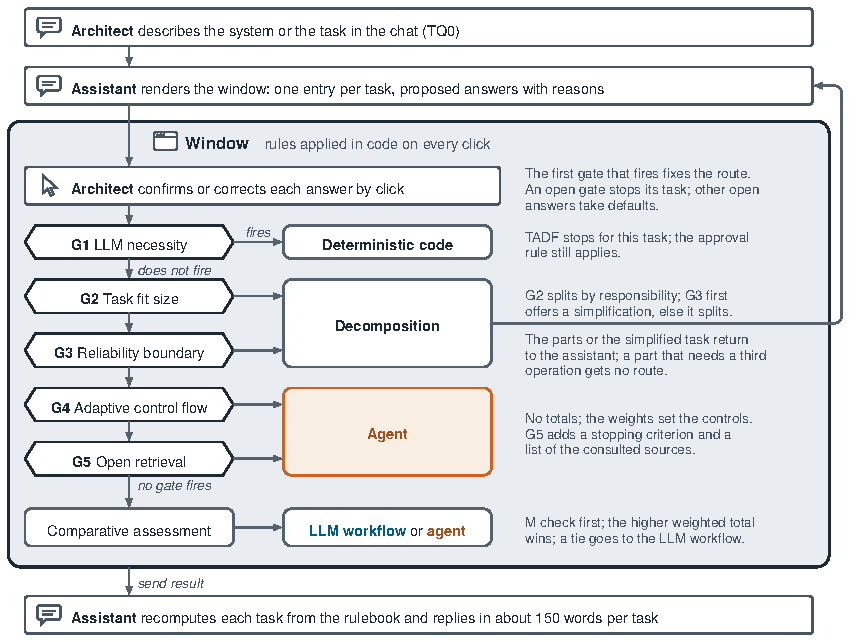
\includegraphics[width=.94\linewidth]{Figures/fig_tadf_final_flow_v2.pdf}
\caption[Routing logic of a TADF consultation in the window]{Routing logic of a TADF consultation in the window, condensed from \texttt{SKILL.md} of the skill \texttt{tadf-final}.}
\label{fig:tadf-flow}
\end{figure}

\subsubsection{Final Capability Matrix and Calculation}
\label{app:artifact/scoring}

Table~\ref{tab:v3-matrix} shows the active matrix. T1 carries weight 3 if its condition is confirmed and 0 otherwise. The architect weights P1--P6 from 0 to 3 and can mark P1, P2, P3 or P5 as mandatory (M). M is accepted only if no later control fully absorbs a violation; otherwise weight 3 applies. The skill calls P1--P6 task-performance indicators, while the thesis calls them deployment indicators.

\begingroup\renewcommand{\baselinestretch}{1}\small\setlength{\tabcolsep}{3pt}\renewcommand{\arraystretch}{1.08}
\begin{longtable}{>{\raggedright\arraybackslash}p{\dimexpr0.070\linewidth-2\tabcolsep\relax} >{\raggedright\arraybackslash}p{\dimexpr0.370\linewidth-2\tabcolsep\relax} >{\raggedright\arraybackslash}p{\dimexpr0.220\linewidth-2\tabcolsep\relax} >{\raggedright\arraybackslash}p{\dimexpr0.100\linewidth-2\tabcolsep\relax} >{\raggedright\arraybackslash}p{\dimexpr0.120\linewidth-2\tabcolsep\relax} >{\raggedright\arraybackslash}p{\dimexpr0.120\linewidth-2\tabcolsep\relax}}
\caption[Capability matrix of the final TADF]{Capability matrix of the final TADF. W: LLM workflow; A: agent.}\label{tab:v3-matrix}\\
\toprule
\textbf{ID} & \textbf{Criterion or deployment indicator} & \textbf{Weight} & \textbf{M allowed} & \textbf{W} & \textbf{A} \\
\midrule
\endfirsthead
\multicolumn{6}{l}{\tablename~\thetable{} (continued)}\\
\toprule
\textbf{ID} & \textbf{Criterion or deployment indicator} & \textbf{Weight} & \textbf{M allowed} & \textbf{W} & \textbf{A} \\
\midrule
\endhead
\bottomrule
\endlastfoot
T1 & Rule application success & 3 if applicable & -- & 3 & 2 \\
\addlinespace
P1 & Traceability & 0--3 or M & yes & 3 & 2 \\
\addlinespace
P2 & Safe failure & 0--3 or M & yes & 3 & 1 \\
\addlinespace
P3 & Schema guarantee & 0--3 or M & yes & 3 & 2 \\
\addlinespace
P4 & Efficiency & 0--3 & no & 3 & 2 \\
\addlinespace
P5 & Robustness to messy input & 0--3 or M & yes & 2 & 3 \\
\addlinespace
P6 & Evolvability & 0--3 & no & 1 & 3 \\
\end{longtable}
\endgroup

For each eligible orchestration paradigm \(p\), the comparative score is
\[
S(p)=\sum_{i\in A}w_i c_{i,p},
\]
where \(A\) contains T1 if it applies and all deployment indicators. M counts as weight 3 but is checked first: capability 1 excludes the orchestration paradigm, and capability 2 makes a control mandatory. The higher total wins, and a tie selects the LLM workflow. A margin of one or two points is checked again and, if it holds, reported as a close call. After the route is fixed, the component rule turns a weight of 2 or more into a mandatory control at capability 2 and into a residual risk that needs a resolution at capability 1. After G4 or G5, M with agent capability 1 is a deployment conflict.

The scores rest on different bases: completion bands at 90 and 50 percent for T1 and P5, construction rubrics for P1 and P3, the observed failure direction for P2, token ratios at 1.5 and 3 times the lower value for P4, and a derivation for P6. They are therefore no common probability scale. At the default weight of 2, the LLM workflow leads by four points and no task-fit criterion favors the agent, so a neutral profile cannot yield an agent recommendation on the comparative path.

\subsubsection{Design Provenance and Evidence Boundaries}
\label{app:artifact/provenance}

Table~\ref{tab:provenance} separates the basis of each design element from the limits of its evidence.

\begingroup
\renewcommand{\baselinestretch}{1}\small
\setlength{\tabcolsep}{3pt}\renewcommand{\arraystretch}{1.08}
\begin{longtable}{>{\raggedright\arraybackslash}p{\dimexpr.24\linewidth-2\tabcolsep\relax} >{\raggedright\arraybackslash}p{\dimexpr.38\linewidth-2\tabcolsep\relax} >{\raggedright\arraybackslash}p{\dimexpr.38\linewidth-2\tabcolsep\relax}}
\caption[Provenance and evidence boundaries of the final TADF]{Provenance and evidence boundaries of the final TADF.}\label{tab:provenance}\\
\toprule
\textbf{Design element} & \textbf{Basis} & \textbf{Evidence boundary}\\
\midrule
\endfirsthead
\multicolumn{3}{l}{\tablename~\thetable{} (continued)}\\
\toprule
\textbf{Design element} & \textbf{Basis} & \textbf{Evidence boundary}\\
\midrule
\endhead
\bottomrule
\endlastfoot
Task as the unit of decision; distinction between the orchestration paradigms & Theoretical background, task taxonomy and the operational definitions of the experiments (Sections~\ref{subsec:theory/workflows-agents}, \ref{subsubsec:TADF/taxonomy}) & A defined scope, not complete coverage of automation architectures. \\
\addlinespace
Gates, T1 and capability scores & Main experimental comparison, deep-dive runs, score rubrics and the initial framework (Sections~\ref{subsubsec:TADF/results}, \ref{subsec:TADF/initial-artifact}) & The gates generalize from selected conditions. P1 and P3 rest on construction, and P6 is derived. The third G3 condition has no measured basis and is kept as a precaution (IT-086). \\
\addlinespace
Skill delivery, system context, definitions and design knowledge & Practitioner interviews and redesign (Section~\ref{subsubsec:TADF/episode1}) & Formative requirements; no comparative usability test and no new capability measurement. \\
\addlinespace
Second G4 question, mandatory minimum and implementation commitment & WorkBench failure diagnosis and executor revision (Section~\ref{subsubsec:TADF/episode2}) & One combined revision without tests of single rules. The measured executor checked conditions and item counts only through prompts, and the new G4 question was not tested again. \\
\addlinespace
Gate block, order of P1--P6, probe for mandatory markings, output structure and fixed-score rule & Pilot consultations and the walkthrough of 27 August 2026 (IT-079 to IT-081; Appendix~\ref{app:artifact/versions}) & Scripted use; independent use and consultation effort were not measured. \\
\addlinespace
Retirement of T3 and T2 & Final structured-retrieval results (49/75 versus 58/75, both band 2) and a confirmation test that gave all nine records the same value (Section~\ref{subsubsec:TADF/evolution}) & Retrieval over known sources and per-item processing remain build knowledge. A new task-fit criterion would need new measurements. \\
\addlinespace
Corrected evidence texts & The defective outcome check of f-med-5 (Appendix~\ref{app:results/contrasts}), the classification of the agent's wrong decisions in D and the records of Episode~2 (IT-084, IT-085) & No score or rule changed. \\
\addlinespace
Consultation window, proposed answers with reasons, rule application in code and short replies & Course and effort of the text consultations of 29 September 2026 (\mbox{IT-087}), the deviations of the walkthrough (\mbox{IT-081}) and the tests of the window against the rulebook (\mbox{IT-088} to \mbox{IT-090}) & Needs a host that can show interactive pages. The effort is compared on two known scenarios with the builder as architect (Section~\ref{subsubsec:TADF/artifact-correction}); independent use was not tested. \\
\end{longtable}
\endgroup

The mandatory minimum combines responses to observed failures with requirements that go beyond the measured executor. The increase from 41.6 to 66.2 percent on WorkBench therefore does not isolate single controls. Likewise, separate calls per criterion in the verification form are a proposed build form: the verification workflow of the main experimental comparison evaluated its five criteria in one structured call before deterministic aggregation (Appendices~\ref{app:protocol/implementation} and~\ref{app:eval2/revision}). A build form, a score threshold or a mandatory component is design knowledge, not verified behavior of a deployed implementation.

\subsubsection{Versions and Iterations}
\label{app:artifact/versions}

Table~\ref{tab:tadf-versions} lists the main states of TADF, their form and how each was assessed. Appendix~\ref{app:evolution/development} details the versions up to v2.2, and Appendix~\ref{app:eval1/improvements} lists the changes after Episode~1. After Episode~2, IT-078 sharpened G4, added the mandatory minimum and the implementation commitment (Section~\ref{subsubsec:TADF/episode2}) and added two build rules: a pilot before an implementation is frozen, and aggregates and superlatives computed in code. It added no gate, threshold, capability score or weight, and it rejected a lifecycle gate, because the lifecycle belongs to the system context. Two simulated pilot consultations on 27 August 2026 then refined the dialogue (IT-079, IT-080). Since then, the deployment indicators are asked in order, explanations are shorter, mandatory markings are task-local and percentages are labelled as comparative fit. Proposed gate answers are confirmed together, and before a mandatory marking is accepted, a probe asks whether a later control absorbs a violation. Replacing selected mandatory markings of safe failure by weight~3 left the recommendations of the pilots unchanged. Their transcripts are not archived. The walkthrough of 27 August 2026 led to the fixed-score rule (IT-081; Appendix~\ref{app:transcripts/audit}). The development log records every iteration with its reason and its change (Appendix~\ref{app:repository/audit}).

\begin{table}[htbp]
\centering
\caption[Versions of TADF, their form and their assessment]{Versions of TADF, their form and their assessment.}
\label{tab:tadf-versions}
\begingroup
\renewcommand{\baselinestretch}{1}\small
\setlength{\tabcolsep}{3pt}
\renewcommand{\arraystretch}{1.08}
\begin{tabular}{>{\raggedright\arraybackslash}p{\dimexpr.22\linewidth-2\tabcolsep\relax} >{\raggedright\arraybackslash}p{\dimexpr.43\linewidth-2\tabcolsep\relax} >{\raggedright\arraybackslash}p{\dimexpr.35\linewidth-2\tabcolsep\relax}}
\toprule
\textbf{Version and date (2026)} & \textbf{Form} & \textbf{Assessment} \\
\midrule
v1 to v2.1, from 15~July & Routing questions in four drafts (list, decision tree, process view and decision table), then gates and weighted scoring in two tables & Deep-dive runs and a structured self-review (Appendix~\ref{app:evolution/development}) \\
\addlinespace
v2.2, frozen on 3~August & Decision Sheet: an Excel workbook that checks five gates for one task and then compares weighted totals & Mechanical checks; Episode~1, practitioner interviews (Section~\ref{subsubsec:TADF/episode1}) \\
\addlinespace
v3, frozen on 25~August & Skill for an LLM assistant: a guided consultation as a text dialogue, plus a headless mode & Episode~2, WorkBench, in benchmark mode (Section~\ref{subsubsec:TADF/episode2}) \\
\addlinespace
v3, revised from 27~August to 29~September & The same skill, revised after Episode~2 and corrected in an evidence audit & Pilot consultations and a walkthrough; text consultation on two scenarios (Appendix~\ref{app:transcripts}) \\
\addlinespace
v3, final state of 1~October & The skill \path{tadf-final}: one consultation window, with a text mode and a headless mode for other uses & Tests of the window code (Appendix~\ref{app:artifact/files}); demonstration (Section~\ref{subsubsec:TADF/artifact-procedure}) \\
\bottomrule
\end{tabular}
\endgroup
\end{table}

\subsection{Demonstration Record and Verification}
\label{app:transcripts}

This appendix documents the text consultations of 29 September 2026 and the window consultations of 1 October 2026, which Sections~\ref{subsubsec:TADF/artifact-correction} and~\ref{subsubsec:TADF/artifact-procedure} summarize. It identifies the transcripts, shows further parts of the text consultations and checks the recorded decisions against the rulebook. The complete dialogues are in the repository (Appendix~\ref{app:repository}).

\subsubsection{Sources}
\label{app:transcripts/source}
\label{app:transcripts/context}

The two text consultations took place on 29 September 2026 in the Claude app with Claude Sonnet~5.5 and the text-interview skill in the state after \mbox{IT-086} (\path{01-framework/tadf/}). The model was confirmed separately, because the export does not record it. The two window consultations followed on 1 October 2026 with the same model and the skill \path{tadf-final/} in the state of \mbox{IT-090}, which the app held as an account plugin with the same files; the memory of the account was off. The Claude data exports contain account data, such as the account identifier, and are therefore not published; the development log records their checksums (IT-087, IT-091). The repository holds Markdown transcripts converted from them in \path{01-framework/demonstration/}, together with the unchanged export of the walkthrough of 27 August 2026 and the checksums of all transcripts. The transcripts keep the visible messages in their original wording and order and omit internal reasoning, file access, tool results and account data. The window transcripts also show the proposed answers of each window as a table and the messages that the window sent to the chat. Messages are numbered from 1 in each transcript, and the figures refer to these numbers. The figures keep the original wording of the messages and mark cuts with [\ldots].

The file-access records of the exports show that the assistant read the procedure, the rulebook and the design knowledge completely in both text consultations, and the document on constructs and scope in the invoice consultation. The text it read matches the files in \path{01-framework/tadf/}, except for the name line at the top of \path{SKILL.md}, which the installation of the skill writes with quotation marks. In the window consultations, every line of the skill files that the assistant read matches the state of \mbox{IT-090}, and both windows equal its template with the window data. Timestamps in the transcripts are Europe/Berlin time. The consultation times in Section~\ref{subsubsec:TADF/artifact-correction} were measured from the timestamps of the exports, without pauses of more than 15 minutes; words count the messages of the assistant without the window code and without the placeholder lines of the export. \path{01-framework/demonstration/consultation-effort/} holds the measured values and the script that measured them.

\subsubsection{Invoice Consultation}
\label{app:transcripts/invoice}

Figure~\ref{fig:demo-invoice-opening} shows how the system context and the task list arose from the first message. Figure~\ref{fig:demo-invoice-record} shows further design knowledge from the verdict and the decision record. The architect confirmed the implementation commitment with the German word ``ja'', and the assistant then wrote the decision record in German. It summarizes the English verdict of message~10.

\begin{figure}[htbp]
\centering
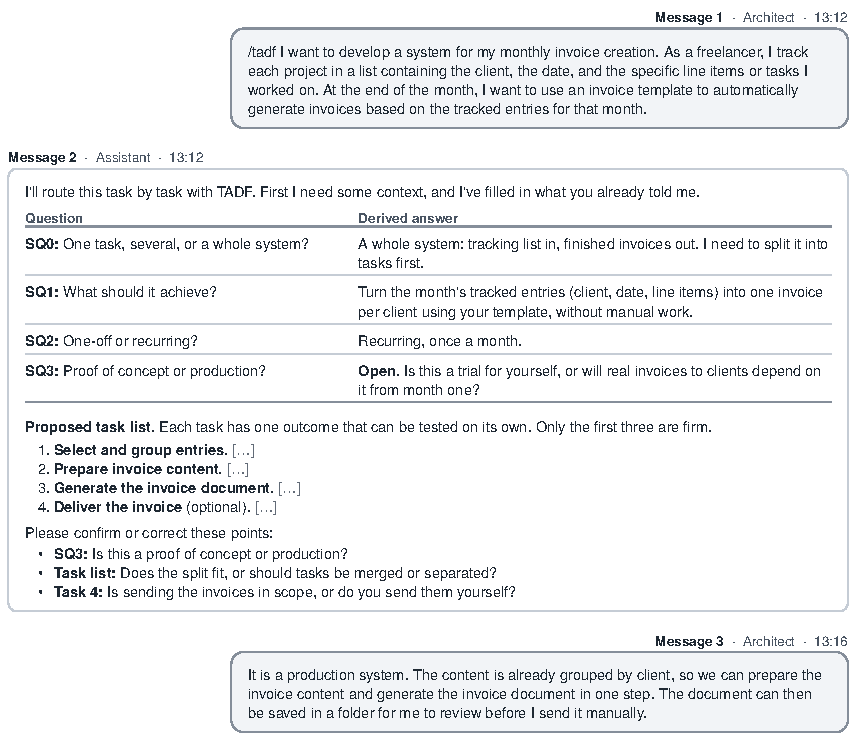
\includegraphics[width=.98\linewidth]{Figures/fig_demo_invoice_opening_v2.pdf}
\caption[Invoice consultation: system context and task list]{Invoice consultation, messages 1--3: system context and task list.}
\label{fig:demo-invoice-opening}
\end{figure}

\begin{figure}[htbp]
\centering
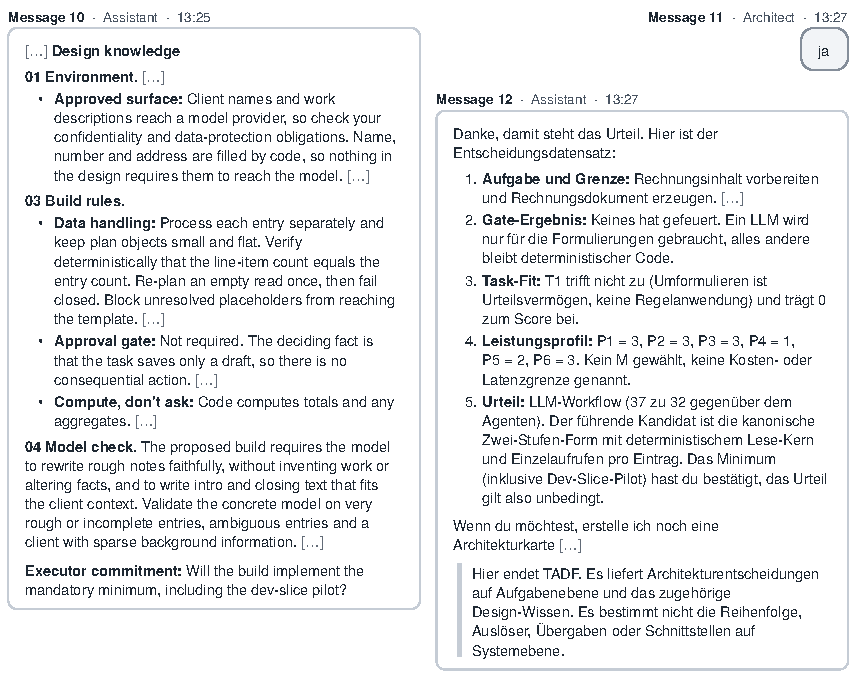
\includegraphics[width=.98\linewidth]{Figures/fig_demo_invoice_record_v2.pdf}
\caption[Invoice consultation: design knowledge and decision record]{Invoice consultation, messages 10--12: design knowledge and decision record.}
\label{fig:demo-invoice-record}
\end{figure}

\subsubsection{CrewAI Consultation}
\label{app:transcripts/crewai}

The scenario was based on \texttt{email\_\allowbreak auto\_\allowbreak responder\_\allowbreak flow}, a publicly available example of CrewAI that checks incoming emails and generates draft responses \parencite{crewaiEmailAutoResponderFlow}. The architect's answers specify the detailed requirements, including human review before sending. They do not describe the behavior of the CrewAI code, which was not evaluated. The same scenario had served in the walkthrough of 27 August 2026.

Figure~\ref{fig:demo-crewai-context} shows the routing of Context gathering. The architect corrected G2 and already named the agent route, but the assistant first clarified G3, because the gates apply in a fixed order. The mandatory marking of safe failure then conflicted with the agent route. The architect resolved the conflict by moving the final readiness decision to deterministic checks outside the loop. The assistant recorded as residual risk what these checks cannot detect, such as a relevant source that was never selected.

For Draft composition, the assistant first counted six simultaneous requirements with a revision round (message~32). The architect answered that code handles exact values, formatting and the output schema and that the model receives one communication profile. The assistant classed this as a simplification that changes the task, the second and last operation on this lineage, and asked which properties the profile fixes and who resolves it (message~34). The architect answered that code resolves the profile from a configuration, which left four requirements, and G3 did not fire (message~36). Figure~\ref{fig:demo-crewai-map} reproduces the architecture map of the closing message.

\begin{figure}[htbp]
\centering
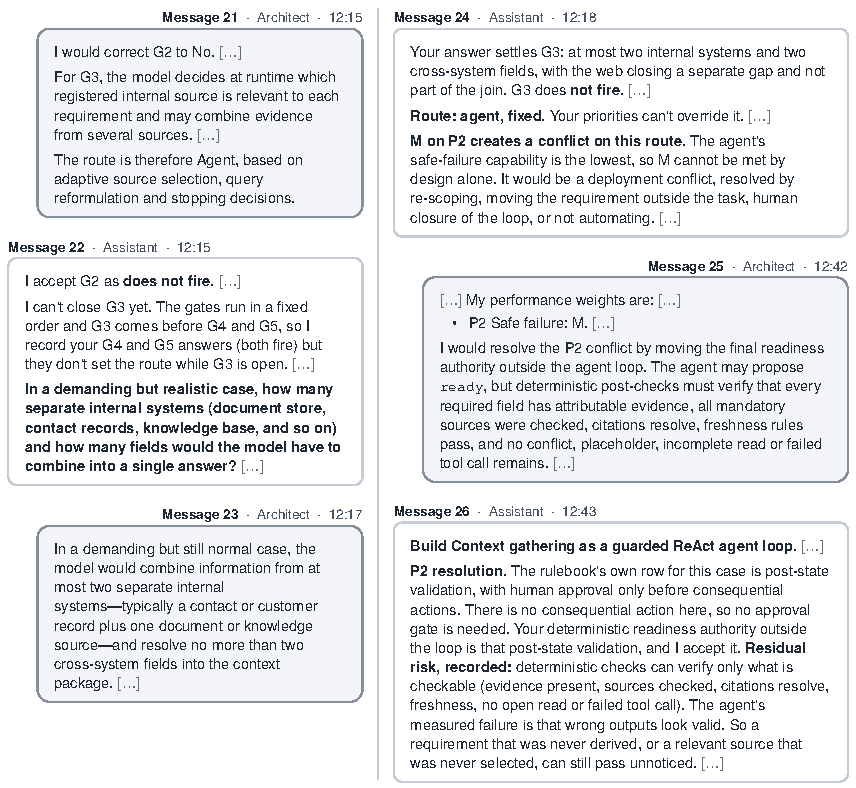
\includegraphics[width=.98\linewidth]{Figures/fig_demo_crewai_context_v2.pdf}
\caption[CrewAI consultation: routing of Context gathering]{CrewAI consultation, messages 21--26: routing of Context gathering.}
\label{fig:demo-crewai-context}
\end{figure}

\begin{figure}[htbp]
\centering
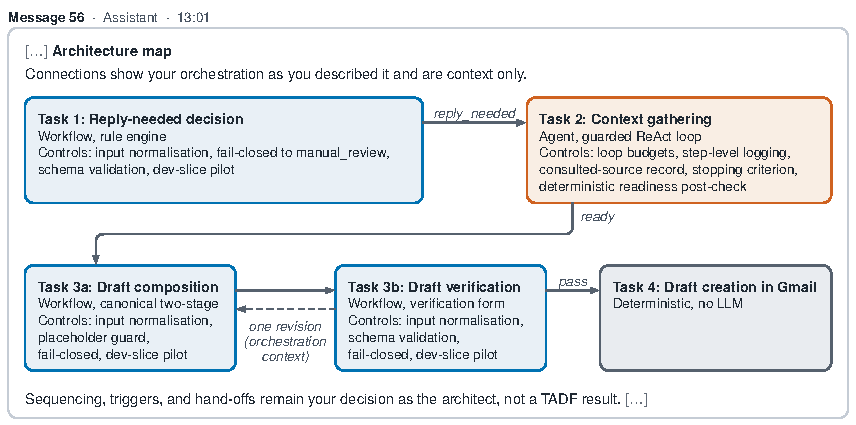
\includegraphics[width=.98\linewidth]{Figures/fig_demo_crewai_map_v2.pdf}
\caption[CrewAI consultation: architecture map]{CrewAI consultation, message 56: architecture map. Node texts, edge labels and connections are those of the Mermaid source; the two-row layout and the colors that mark the three routes were added for the page.}
\label{fig:demo-crewai-map}
\end{figure}

\subsubsection{Decision and Procedure Verification}
\label{app:transcripts/audit}

Table~\ref{tab:demo-audit} checks the recorded decisions against the rulebook. All totals were recomputed from the fixed capability scores and the confirmed weights. The table does not validate the factual answers of the architect.

\begingroup
\renewcommand{\baselinestretch}{1}\small
\setlength{\tabcolsep}{3pt}\renewcommand{\arraystretch}{1.08}
\begin{longtable}{>{\raggedright\arraybackslash}p{\dimexpr.20\linewidth-2\tabcolsep\relax} >{\raggedright\arraybackslash}p{\dimexpr.34\linewidth-2\tabcolsep\relax} >{\raggedright\arraybackslash}p{\dimexpr.46\linewidth-2\tabcolsep\relax}}
\caption[Check of the text consultations against the rulebook]{Check of the text consultations against the rulebook.}\label{tab:demo-audit}\\
\toprule
\textbf{Task and messages} & \textbf{Recorded outcome} & \textbf{Check and limit} \\
\midrule
\endfirsthead
\multicolumn{3}{l}{\tablename~\thetable{} (continued)}\\
\toprule
\textbf{Task and messages} & \textbf{Recorded outcome} & \textbf{Check and limit}\\
\midrule
\endhead
\bottomrule
\endlastfoot
Invoice creation (1--12) & No gate fired; T1 did not apply. P1--P6 weighted 3, 3, 3, 1, 2, 3. LLM workflow, 37 to 32. & Workflow: $9+9+9+3+4+3=37$. Agent: $6+3+6+2+6+9=32$. Input normalization is mandatory (P5), and evolvability is a residual risk (P6). The architect confirmed complete reads with a general answer; the build form still requires reading all pages. \\
\addlinespace
Reply-needed decision (8--17) & No gate fired; T1 applied. P2 and P3 mandatory. LLM workflow with rule engine, 50 points. & $9+9+9+9+6+6+2=50$. P2 as M excludes the agent at capability 1, and the agent columns hold no values. P3 as M alone would have kept the agent eligible. \\
\addlinespace
Context gathering (18--26) & G4 fired, and G5 was recorded. P2 mandatory. Agent, guarded ReAct loop. & The route is fixed, so there is no total. M with agent capability 1 after G4 is a deployment conflict, resolved here by post-state validation. The proposed checks are a design, not a tested control, and cannot show that no relevant source was missed; the verdict records this residual risk. \\
\addlinespace
Draft writing (26--30) & G2 fired. Decomposition into Draft composition and Draft verification. & The parent receives no profile. This is the first operation on the lineage. \\
\addlinespace
Draft composition (30--41) & Simplification, then no gate. P1--P6 weighted 3, 3, 3, 2, 3, 2. LLM workflow, canonical two-stage form, 41 to 34. & Workflow: $9+9+9+6+6+2=41$. Agent: $6+3+6+4+9+6=34$. The margin of seven points is not a close call. The simplification was the second and last operation on the lineage. \\
\addlinespace
Draft verification (42--51) & No gate fired; T1 did not apply. P2 and P3 mandatory. LLM workflow, verification form, 41 points. & $9+9+9+6+6+2=41$. P2 as M excludes the agent. Verification parity in cost was named as context, and the score stayed fixed. That three model-judged criteria lie within the measured five-criterion rubric does not validate this rubric. \\
\addlinespace
Draft creation in Gmail (52--56) & G1 fired. Deterministic implementation. & No profile and no design knowledge, as the rulebook prescribes. \\
\end{longtable}
\endgroup

The walkthrough of 27 August 2026 (IT-081) used the same scenario with the state before the fixed-score rule, when T3 and T2 were still scored. Its record showed five deviations: a stated total of 41 whose contributions summed to 50, agent contributions changed through the efficiency exception, values in the columns of an excluded agent, no implementation commitment and no separate G4 question on complete reads. None of them recurred in the repeated consultation. The four verdicts for an LLM workflow cite 41.6 and 66.2 percent success without and with the mandatory minimum. They need the qualification of Appendix~\ref{app:artifact/provenance}: the measured executor implemented parts of the minimum only through prompts. \mbox{IT-089} reduced these sentences in the skill to what the records show.

\subsubsection{Window Consultations}
\label{app:transcripts/window}

The window consultations of 1 October 2026 used the same two scenarios (\mbox{IT-091}). In each, the assistant showed one window with proposed answers, the architect answered by click and sent the result, and the assistant replied once. The windows proposed 19 and 45 answers. The architect kept 18 and 40 of them, changed 1 and 5 and answered 1 and 18 further questions without a proposal. The architect answered several questions differently from the text consultations. In invoice creation, traceability was weighted 2 and evolvability 1. In the email scenario, the reply-needed decision had no task-fit criterion and no mandatory marking, and draft writing was not split, so its two parts were not routed. Table~\ref{tab:demo-window-audit} checks the recorded decisions against the rulebook. In both consultations, the assistant's recomputation agreed with the window, and no capability score was changed. The assistant pointed out four answers that seemed inconsistent with the description and said whether a change would alter the route, but it left the answers to the architect.

\begingroup
\renewcommand{\baselinestretch}{1}\small
\setlength{\tabcolsep}{3pt}\renewcommand{\arraystretch}{1.08}
\begin{longtable}{>{\raggedright\arraybackslash}p{\dimexpr.20\linewidth-2\tabcolsep\relax} >{\raggedright\arraybackslash}p{\dimexpr.34\linewidth-2\tabcolsep\relax} >{\raggedright\arraybackslash}p{\dimexpr.46\linewidth-2\tabcolsep\relax}}
\caption[Check of the window consultations against the rulebook]{Check of the window consultations against the rulebook.}\label{tab:demo-window-audit}\\
\toprule
\textbf{Task} & \textbf{Recorded outcome} & \textbf{Check and note} \\
\midrule
\endfirsthead
\multicolumn{3}{l}{\tablename~\thetable{} (continued)}\\
\toprule
\textbf{Task} & \textbf{Recorded outcome} & \textbf{Check and note}\\
\midrule
\endhead
\bottomrule
\endlastfoot
Invoice creation & No gate fired; T1 did not apply. P1--P6 weighted 2, 3, 3, 1, 2, 1. LLM workflow, 32 to 24. & Workflow: $6+9+9+3+4+1=32$. Agent: $4+3+6+2+6+3=24$. Input normalization is mandatory (P5), and evolvability is an accepted limitation (P6). The assistant noted that its proposed weight of 3 for P5 would give 34 to 27. \\
\addlinespace
Reply-needed decision & No gate fired; T1 did not apply. P1--P6 weighted 2, 3, 3, 2, 2, 1. LLM workflow, 35 to 26. & Workflow: $6+9+9+6+4+1=35$. Agent: $4+3+6+4+6+3=26$. The efficiency exception of batch classification was named as context only; the score stayed fixed. The assistant noted its proposed weight of 3 for P5. \\
\addlinespace
Context gathering & G4 fired: the model must replan, and the planned reads cannot show the whole deciding state. Agent, ReAct loop. & The route is fixed, so there is no total. Controls are mandatory for P1, P3 and P4, and P2 at weight 2 is a residual risk. The assistant noted that this weight seemed inconsistent with the fail-closed requirement of the description. \\
\addlinespace
Draft writing & No gate fired, because the architect answered G3a with no instead of the proposed yes. P2 mandatory. LLM workflow, 35; agent excluded. & Workflow: $9+9+9+3+4+1=35$. P2 as M excludes the agent at capability 1. The assistant noted that the seven simultaneous requirements with a revision round described in the task would fire G3. \\
\addlinespace
Draft creation in Gmail & G1 fired. Deterministic implementation. & No profile and no design knowledge, as the rulebook prescribes. \\
\end{longtable}
\endgroup

These records bound the role of the consultations. They show how the instrument elicits requirements, applies its rules and records its decisions. They do not measure the task success, token cost or safety of the recommended builds, and one consultation per scenario does not establish unaided use or reliable application with other models. The window consultations used partly different answers than the text consultations, so they illustrate the effect of the window and do not measure it.
% APPENDIX B
\clearpage

\section{Formal Appendix}
\label{app:Formal A}

\subsection{Eidesstattliche Versicherung}
\label{sec:SOOA}

\vspace{2.5cm}

% Statement of original authorship - Needs to be in German
% see also here: https://www.wiso.uni-koeln.de/sites/fakultaet/dokumente/PA/formulare/eidesstattliche_erklaerung.pdf

Hiermit versichere ich an Eides statt, dass ich die vorliegende Arbeit selbstständig und ohne die Benutzung anderer als der angegebenen Hilfsmittel angefertigt habe. Alle Stellen, die wörtlich oder sinngemäß aus veröffentlichten und nicht veröffentlichten Schriften entnommen wurden, sind als solche kenntlich gemacht. Die Arbeit ist in gleicher oder ähnlicher Form oder auszugsweise im Rahmen einer anderen Prüfung noch nicht vorgelegt worden. Ich versichere, dass die eingereichte elektronische Fassung der eingereichten Druckfassung vollständig entspricht.

\vspace{1cm}

\noindent
Die Strafbarkeit einer falschen eidesstattlichen Versicherung ist mir bekannt, namentlich die Strafandrohung gemäß § 156 StGB bis zu drei Jahren Freiheitsstrafe oder Geldstrafe bei vorsätzlicher Begehung der Tat bzw. gemäß § 161 Abs. 1 StGB bis zu einem Jahr Freiheitsstrafe oder Geldstrafe bei fahrlässiger Begehung.

\vspace{3cm}
\noindent
\textbf{\thesisauthor{}}

\vspace{0.5cm}
\noindent
Köln, den xx.xx.20xx





\end{document}